%% This is file `medima-template.tex',
%%
%% Copyright 2018 Elsevier Ltd
%%
%% This file is part of the 'Elsarticle Bundle'.
%% ---------------------------------------------
%%
%% It may be distributed under the conditions of the LaTeX Project Public
%% License, either version 1.2 of this license or (at your option) any
%% later version.  The latest version of this license is in
%%    http://www.latex-project.org/lppl.txt
%% and version 1.2 or later is part of all distributions of LaTeX
%% version 1999/12/01 or later.
%%
%% The list of all files belonging to the 'Elsarticle Bundle' is
%% given in the file `manifest.txt'.
%%
%% Template article for Elsevier's document class `elsarticle'
%% with harvard style bibliographic references
%%
%% $Id: medima-template.tex 153 2018-12-01 11:38:32Z rishi $
%% $URL: http://lenova.river-valley.com/svn/elsarticle/trunk/medima-template.tex $
%%
%% Use the option review to obtain double line spacing
%\documentclass[times,review,preprint,authoryear]{elsarticle}

%% Use the options 'twocolumn,final' to obtain the final layout
%% Use longtitle option to break abstract to multiple pages if overfull.
%% For Review pdf (With double line spacing)
%\documentclass[times,twocolumn,review]{elsarticle}
%% For abstracts longer than one page.
%\documentclass[times,twocolumn,review,longtitle]{elsarticle}
%% For Review pdf without preprint line
%\documentclass[times,twocolumn,review,nopreprintline]{elsarticle}
%% Final pdf
\documentclass[times,twocolumn,final]{elsarticle}
%%
%\documentclass[times,twocolumn,draft,longtitle]{elsarticle}
%%


%% Stylefile to load MEDIMA template
\usepackage{medima}
\usepackage{framed,multirow}
\graphicspath{{./}{../../templates/MEDIMA-template/}{figures/}}
\usepackage{amssymb,latexsym}
\usepackage[nointegrals]{wasysym}

% Following three lines are needed for this document.
% If you are not loading colors or url, then these are
% not required.
\usepackage{url}
\usepackage{xcolor}
\usepackage{graphicx,amsmath}
\usepackage{subcaption}

\usepackage{hyperref}
\usepackage[nameinlink]{cleveref}
\Crefname{lstlisting}{listing}{listings}
\Crefname{lstlisting}{Listing}{Listings}

\usepackage{tikz}
\usetikzlibrary{positioning,arrows,calc}
\usepackage{listings}
%\renewcommand{\ttdefault}{pcr}
\lstset{
  numbers=left,
  captionpos=b,
  keepspaces=true,
  basicstyle=\scriptsize\ttfamily,
  keywordstyle=\bfseries\ttfamily,
  commentstyle=\color{gray}\ttfamily
}
\usepackage{algorithm}
\usepackage[noend]{algpseudocode}

\definecolor{newcolor}{rgb}{.8,.349,.1}

\journal{Medical Image Analysis}


\usepackage{tikz}
\usetikzlibrary{shapes.geometric}
\usetikzlibrary{arrows.meta,arrows}
\usetikzlibrary{positioning}



%\newcommand{\xx}{\mathbf{x}}
% \newcommand{\fval}{f(\xx)}
% \newcommand{\fval}{f}
%\newcommand{\fval}{x}
%\newcommand{\lab}{\mathrm{L}}
%\newcommand{\micron}{\ensuremath{\mu\text{m}}}
\newcommand{\Pof}[2]{P\!\left(#1\middle\vert #2\right)}
%\newcommand{\voxels}{\mathsf{voxels}}
%\newcommand{\field}{\mathsf{field}}



% \usepackage{showframe} % for debugging
\usepackage{ulem}
\newcommand{\carl}[1]{\textcolor{orange}{[Carl: #1]}}
\newcommand{\aleksandar}[1]{\textcolor{cyan}{[Aleksandar: #1]}}
\newcommand{\james}[1]{\textcolor{red}{[James: #1]}}
\definecolor{ForestGreen}{RGB}{34,139,34}
\newcommand{\suggestion}[3]{\textcolor{ForestGreen}{[\textbf{Suggestion (#1):} '\sout{#2}' $\rightarrow$ '#3']}}


\newcommand{\xx}{\mathbf{x}}
% \newcommand{\fval}{f(\xx)}
% \newcommand{\fval}{f}
\newcommand{\fval}{x}
\newcommand{\lab}{\mathrm{L}}
\begin{document}

\verso{ Avery \textit{et~al.}}

\begin{frontmatter}

% \title{Spatial Analysis for SR$\mu$CT Segmentation}%
\title{
  Reversing distortive X-ray effects I:
  Accurate Implant-contact Tissue Classification in Bone SR$\mu$CT
}%

\author[1,2]{James \snm{Avery}\corref{cor1}}
\cortext[cor1]{Corresponding author:\\
  Address: Universitetsparken 5, 2100 Copenhagen O, Denmark \\
  Email: avery@nbi.ku.dk\\
}
\ead{avery@nbi.ku.dk}
\author[2]{Aleksandar \snm{Topic}}
\ead{aleksandar.topic@nbi.ku.dk}
\author[1]{Carl-Johannes \snm{Johnsen}}
\ead{carl-johannes@di.ku.dk}
\author[3]{Else \snm{Pinholt}}
\ead{empinholt@health.sdu.dk}

\address[1]{University of Copenhagen, Department of Computer Science}
\address[2]{University of Copenhagen, Niels Bohr Institute}
\address[3]{University of Southern Denmark}

\received{30 June 2022}
%\finalform{10 May 2013}
%\accepted{13 May 2013}
%\availableonline{15 May 2013}
%\communicated{S. Sarkar}


\begin{abstract}
  %%%
  Synchrotron Radiation micro-CT (SRµCT) produces 3D images at extremely high
fidelity. While distortive X-ray effects such as beam hardening are minimized
due to the highly brilliant monochromatic beams, they are not eliminated. This
becomes particularly evident when attempting to obtain accurate tissue
classification near high-contrast interfaces, such as those presented by metal
implants.

We present a computational method that discovers image distortion as a function
of space and produces continuous probabilistic models of material
classification functions. Using the derived models, we can accurately classify
tissue throughout the full image, even at high-contrast transition interfaces.
We apply the method to solve the notoriously difficult problem of accurately
classifying biological tissue in contact with a titanium implant.

The new tissue classification method was used to evaluate bone-to-implant
contact (BIC) in micrometer-resolution SRµCT images. In a previous study, we
were unable to obtain accurate results for BIC, due to difficulties in
accurately classifying the tissue types near the titanium implant surface. In
the present work, we invert the distortive effects and obtain accurate tissue
classification close to the implant surface.
%TODO: Issue #1. MANGLER TAL HER. Disse skal beregnes.
The method is open-source, implemented in C++ and Python, and targets
out-of-core execution on multi-core CPU and multi-GPU systems.

%%% Local Variables:
%%% mode: latex
%%% TeX-master: "main"
%%% End:

%%%%
\end{abstract}

\begin{keyword}
%% MSC codes here, in the form: \MSC code \sep code
%% or \MSC[2008] code \sep code (2000 is the default)
%\MSC 41A05\sep 41A10\sep 65D05\sep 65D17
\MSC 92C55\sep 62H35\sep
%% Keywords
\KWD Image analysis \sep Tissue classification \sep Ossointegration \sep Segmentation \sep Bone-to-implant contact \sep Synchrotron Radiation micro-CT
\end{keyword}

\end{frontmatter}

%\linenumbers

\section{Introduction}
\label{sec:intro}

Bone samples are most commonly analyzed by extracting histologies and examining
their two-dimensional structure with light microscopy. This method has several
drawbacks. First and foremost, it is destructive: In addition to the obvious
issue that the histology must be cut from the full sample, the sawing process
can contaminate soft tissue with bone dust, or leave surface scratches that
complicate automatic image analysis. Secondly, histology by its nature only
gives a two-dimensional slice of the full three-dimensional picture - most
important biological structures are inherently three-dimensional, and limiting
analysis to 2D severely restricts the types of questions we can answer.

Synchrotron Radiation micro-tomography (SRµCT) offers a non-destructive
high-quality alternative to histology for detailed analysis of bone biopsies.
\cite{torsten2018} quantified the uncertainty of 2D histology for four common
bone analyses, and found that the choice of sampling plane for histological
analysis incurred a significant uncertainty in the results, whereas the full
volumetric analysis of SRµCT tomograms did not.

The high brilliance and collimation of synchrotron radiation yields
particularly faithful 3D images, as common distortive X-ray effects seen in
hospital-grade setups such as beam hardening and projection artifacts are
minimized. The high fidelity makes SRµCT attractive for conducting advanced
medical image analyses with trustworthy results.

However, while image distortion effects are much reduced compared to laboratory
X-ray tomography, they are not eliminated, and numerical analysis and
computations on the images must still be conducted carefully. Boundary effects
near sample surfaces, ring artifacts from sensor faults, and especially
distortion near high-contrast transitions, make accurate tissue classification
difficult in regions where this distortion is significant. \cite{sporring}
found that, while they could accurately classify bone tissue in the middle
regions of the tomograms, they were not able to obtain good bone-to-implant
contact evaluation (BIC), as evidenced by poor correlation with histological
analysis of the same samples.

% TODO: PLACEHOLDER FOR LITERATURE REVIEW - why are the current methods not good enough?
% 
% Include weaknesses and limitations of:
%  - Morphology-based-article
%  - software approaches: Pore3D, Avizo, ITK-Snap, ..., no one-fits-all program
%     - most are proprietary software, time-consuming and manual work already for much smaller volumes
%  - ML-based-article with U-net
%  - include article G with their systematic literature review also

The present work presents a fully automatic computational method which
discovers probabilistic models for the distortions incurred by the physical
effects in high-resolution X-ray CT such as SRµCT to reverse them and
produce accurate tissue classification even in regions where these effects are
significant. It exploits two properties, which are needed to hold for the
method to work: i) very high resolution is used to build statistical models as
functions of space, and ii) the effects to be countered must vary continuously
over space so that we can track how voxel frequency distributions are distorted
throughout the image. We apply the method to the same dataset of
micrometer-resolution SRµCT bone tomograms studied in \cite{torsten2018}
and in \cite{sporring}, to achieve faithful tissue classification close to the
titanium implant surface. The implementation is open-source, targets multi-CPU
and multi-GPU systems, and is available at
\href{https://github.com/jamesavery/maxibone}
{https://github.com/jamesavery/maxibone}.

%%% Local Variables:
%%% mode: latex
%%% TeX-master: "main"
%%% End:


\section{Background}
\label{sec:background}

In this section, we will briefly go through the physical composition of our samples, and how the
data is acquired. Then we will look at the noise sources typical for this type of data, and show
the effects that noise has on regions around the implant and biological tissue.

\subsection{Data set}


Seven goats got introduced 5 critical size defects, with bone being cut accordingly in the region.
 Four defects were used to asses bone regeneration methods, and one was a control sample.
 Peri-implant vertical bone augmentation was performed using autologous bone and two different
 calcium phosphate bone substitutes. The bone specimens were evaluated undecalcified. The
 specimen preparation was performed at the Department of Biomaterials at Gothenburg University,
 Sweden. The specimens were initially fixated in 4\% paraformaldehyde. Dehydration of the
 specimens was performed in increasing concentrations of ethanol to eliminate fat and water
 content. Furthermore, specimens were infiltrated with MMA and embedded in molds 12 mm in
 diameter and 20 mm in height \james{(Donath 1982, 1993, Erben 1997)}. They were scanned at the ESRF
 in Grenoble, France. The advantage of using MMA is greater tissue penetration than water-soluble
 methacrylates this is an advantage when preparing larger specimens such as bone biopsies
 containing dental implants. Furthermore, the histological quality of bone sections is generally
 higher for MMA embedded specimens compared to water- soluble methacrylates \james{(Erben 1997)}.
 Additionally, tissue shrinkage is less than 2\% when using MMA embedded bone and cartilage
 specimens \james{(Ferguson et al. 1999)}.


As the specimen for X-ray imaging included a titanium dental implant, comparatively high photon
 energy of 67.4 KeV (pink) \aleksandar{Hov! Vi blev enige om 50 KeV ???} was chosen, i.e. the
 emitted radiation of a wiggler insertion device (a
 magnetic device) was filtered    to produce a narrower bandwidth. An indirect detector (lens-coupling
 of a scintillator to a camera incorporating a charge-coupled device with $2048 \times 2048$ pixels),
 with a pixel size of 5$\mu$m acquired tomographic scans of the ROI, which was slightly smaller (10mm wide)
 than the specimen (~20mm wide)” (Neldam et al. 2015). The sample was continuously rotated over
 180 degrees, as 1999 equiangular spaced radiographic images were taken.

\subsubsection{Physical samples}

The physical samples were prepared for SR$\mu$CT scanning by cutting out a portion from a larger
12mm cylindrical sample. The cut samples are cubes of size (6.478mm, 6.478mm, 6.146mm) in the
$(x,y,z)$ direction respectively. This contains the titanium dental implant (Astra Tech OsseoSpeed,
ST Molndal, Sweden), which is 3.5mm in diameter and 8mm long. Along its length the lower 5.5mm
has larger threads and is attached to recipient bone. The upper 2.5mm has smaller threads and
is where newly formed bone is to be assessed. Sorrounding the bone and implant contact-region
are cavities containing resin, air, blood vessels and other fibrous tissue.

\begin{figure}
\centering
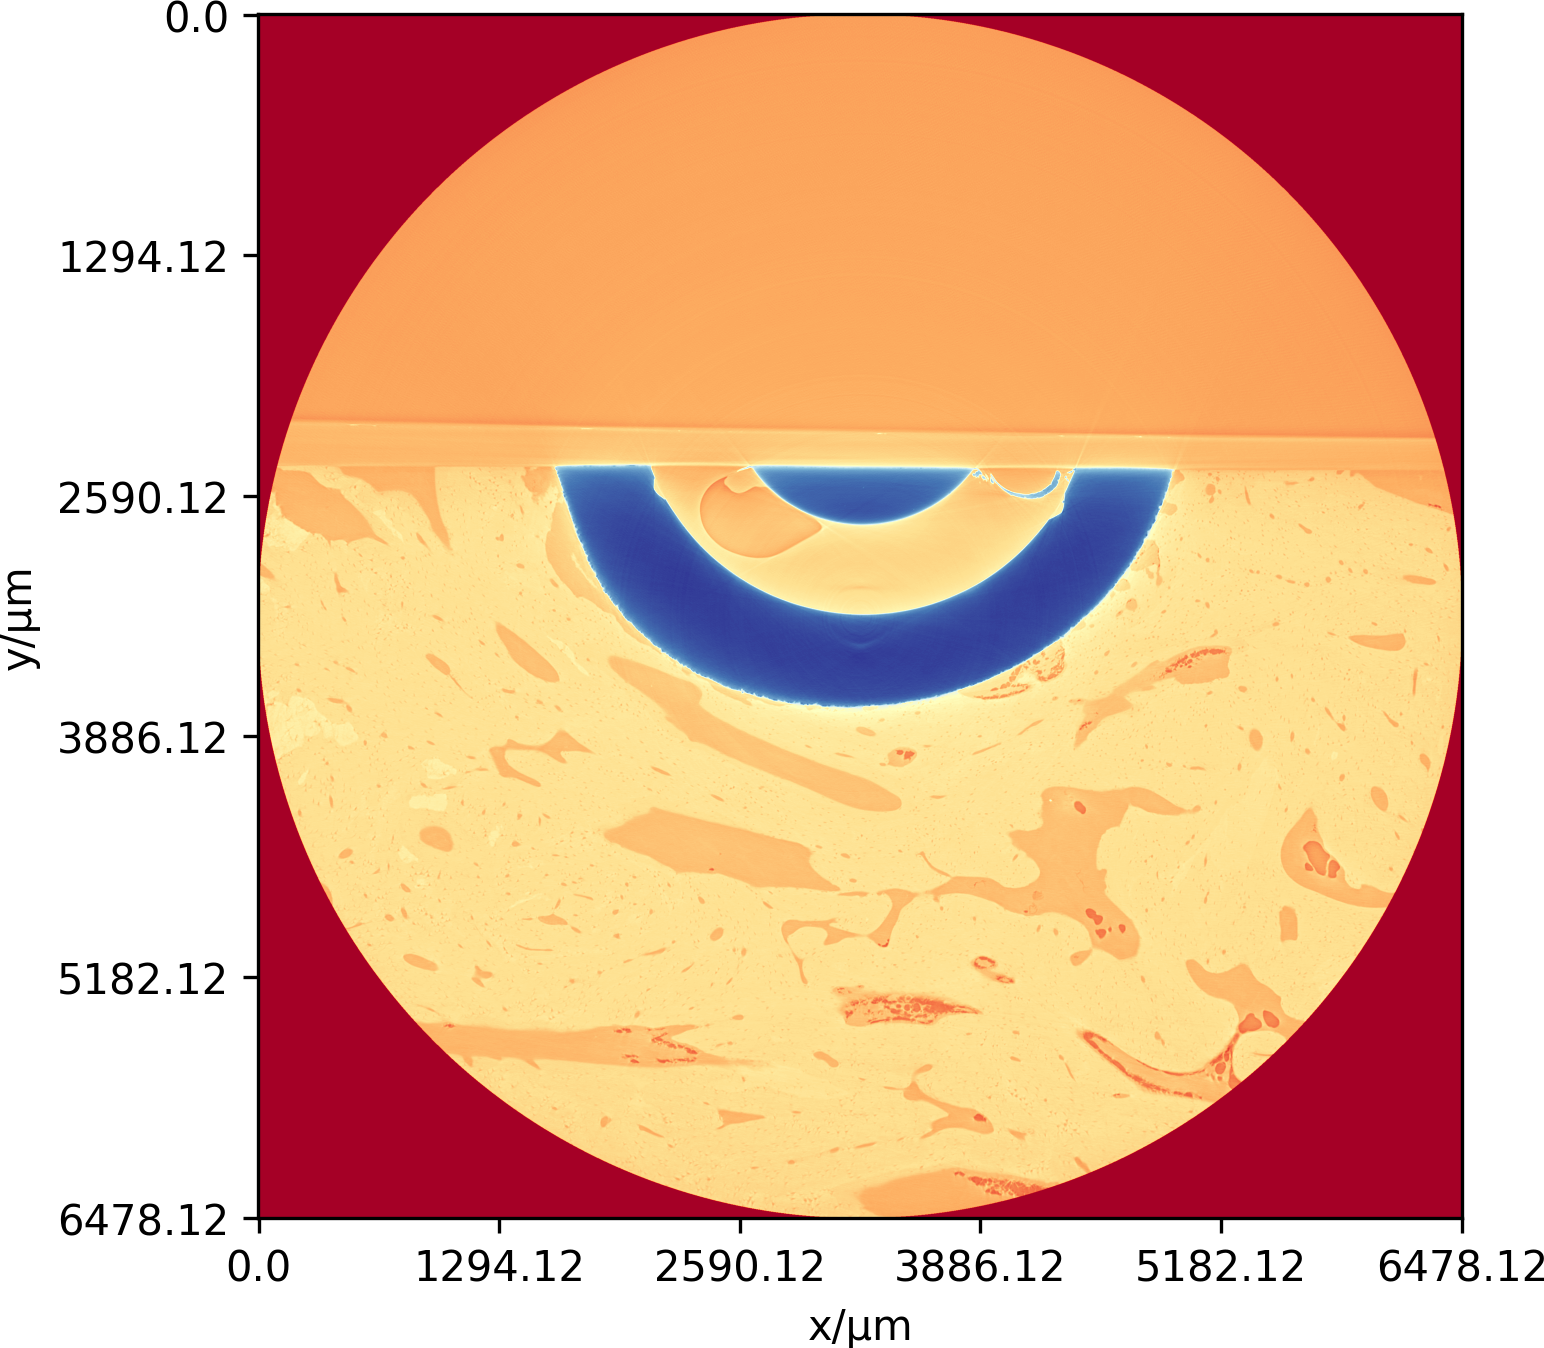
\includegraphics[width=0.96\columnwidth]{770c_pag-full-xy-1x.png}
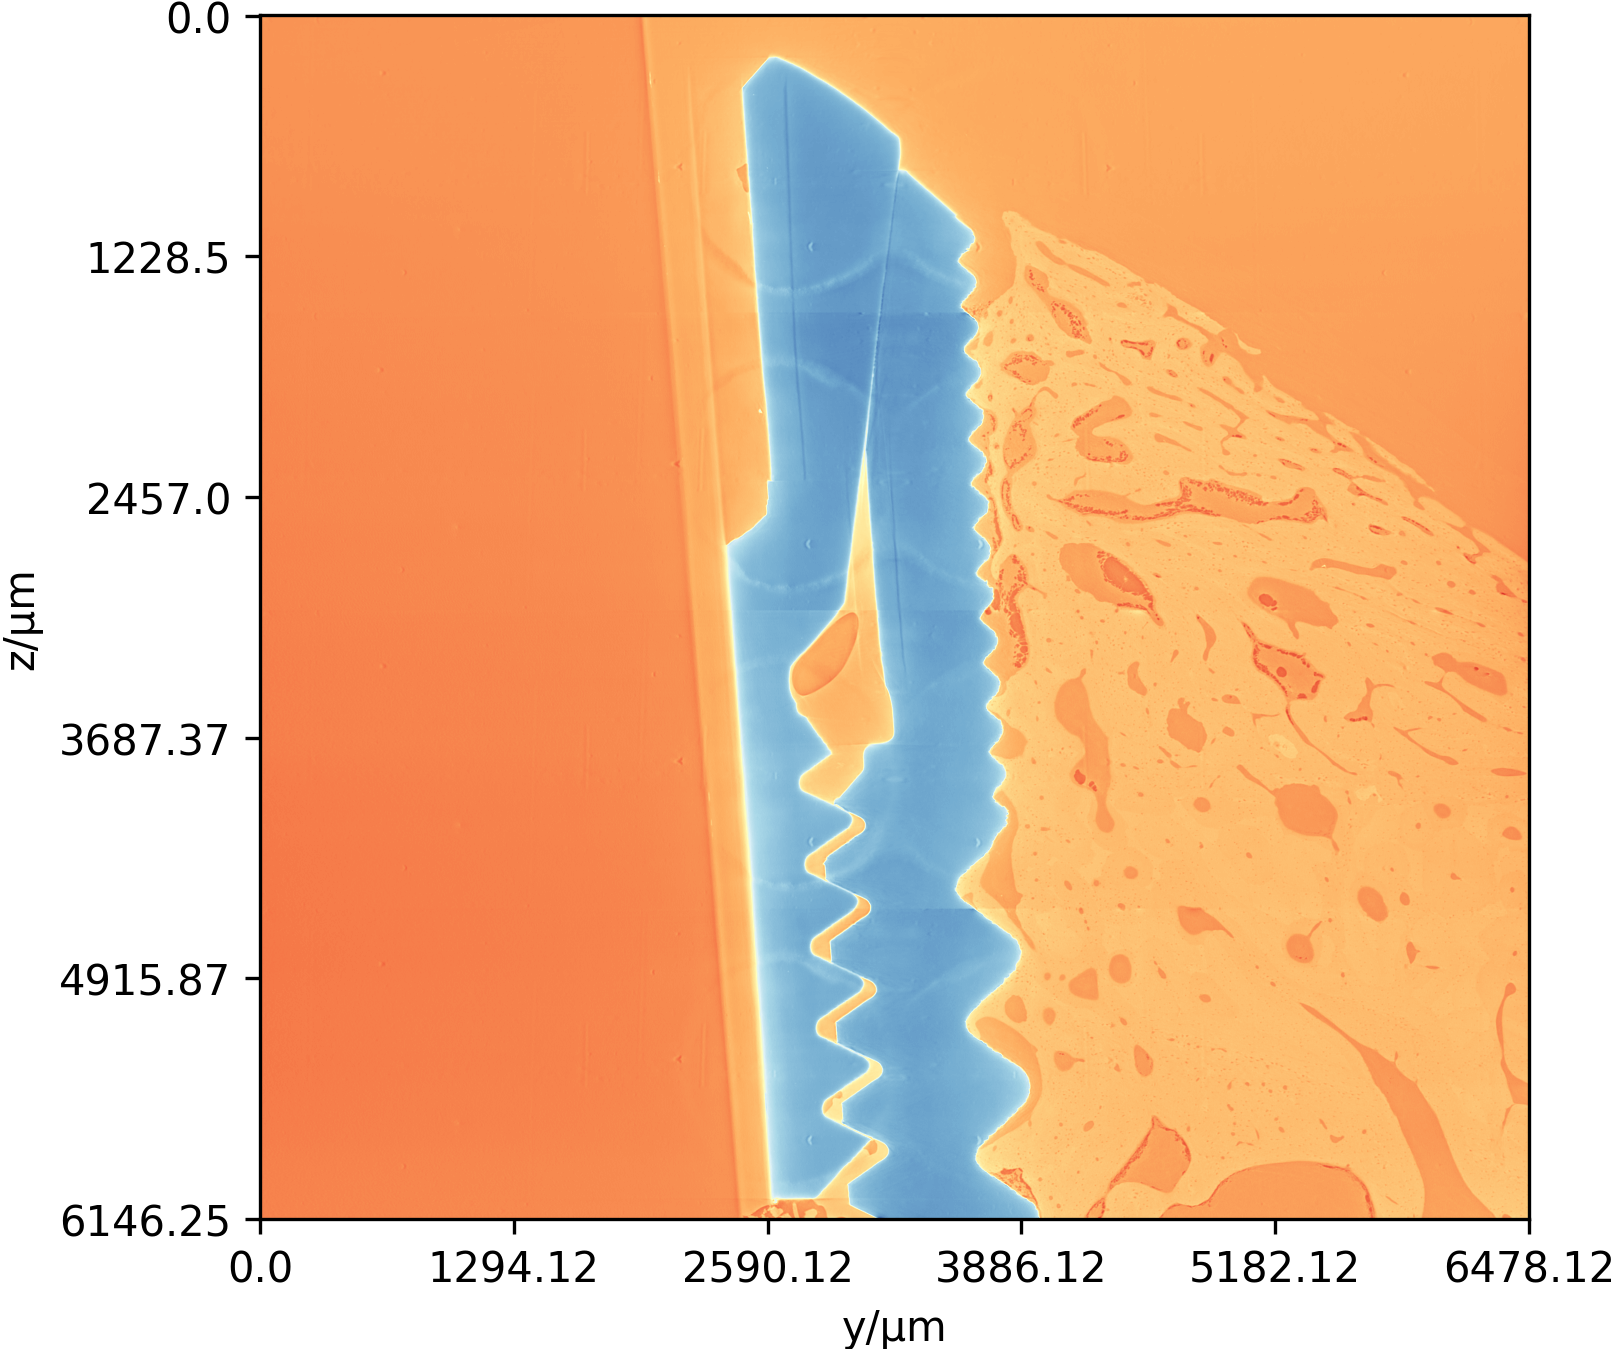
\includegraphics[width=0.96\columnwidth]{770c_pag-full-yz-1x.png}
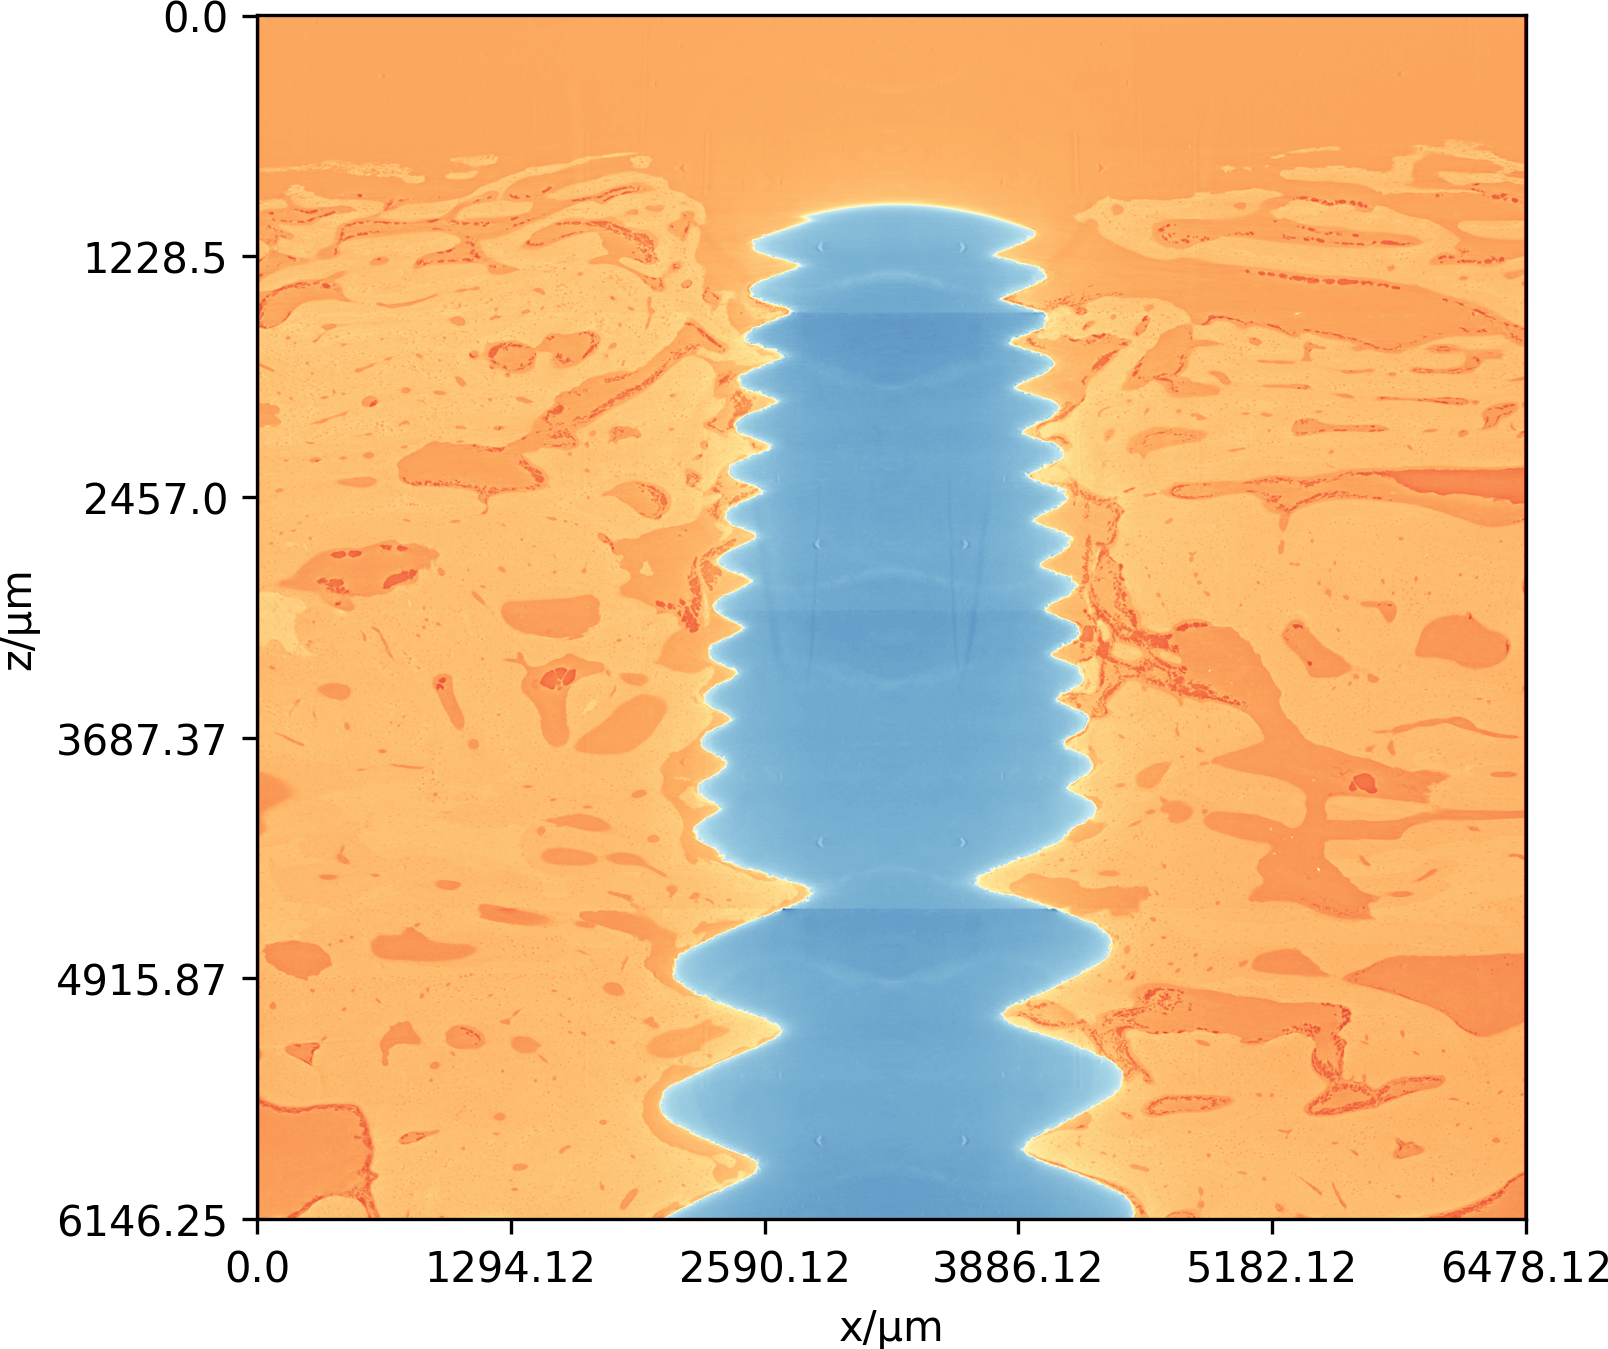
\includegraphics[width=0.96\columnwidth]{770c_pag-full-xz-1x.png}
\caption{Cut sample seen as cross sections in XY, YZ and XZ-planes respectively. A voxel has a size
of 1.875$\mu$m. Red voxels are numerically low, while blue voxels are high.}
\label{fig:3viewsample}
\end{figure}

A cut sample is shown in three different cross sectional views in \cref{fig:3viewsample}. Each
material has a unique density and thus absorption. The titanium implant shown in blue has a
higher absorption level than bone. Bone material shown in light orange has higher absorption
than its sorrounding dark orange colored regions containing blood vessels tissue, air and resin.

\subsubsection{Data acquisition}

It can be difficult to study and evaluate the bone structure and blood network without destroying
or manipulating the sample. X-ray computed tomography is a widely used tool for non-intrusive medical
imaging. By exposing a subject to X-rays, we can map the linear attentuation coffecient of the passing
rays. Each ray is attenuated relatively to the density and composition of the material it passes.
By rotating either the scanner or the sample we can get a full 3D image representation of the inner
structure of the sample. Each volumetric pixel (voxel) then represents the X-ray attenuation at its
spatial position. We can therefore reliably use X-rays to internally characterise samples in a
non-intrusive and non-destructive manner. Medical CT-scans can provide spatial resolutions on the
order of submillimetre scale \citep{medicalct}. The more modern micro computed tomography ($\mu$CT)
can provide much higher spatial resolution on the micrometre scale \citep{srexptime}.

This work focuses on a data set acquired by Synchrotron Radiation micro-CT (SR$\mu$CT). For this
imaging technique, electrons are accelerated to ultra-relativistic speeds in trajectories directed
by strong magnetic fields. The resulting X-ray beam provides a high photon flux allowing for very
short exposure times \citep{srexptime}. This can help counter Poisson noise from suboptimal photon
count \citep{srnoise}. Contrary to both CT and $\mu$CT, this approach requires a large particle
accelerator, and is not standard medical or laboratory equipment. However, SR$\mu$CT  offers an
even better spatial resolution of up to 0.1 $\mu$m, and much higher image quality due to fewer
distortive X-ray effects. The resulting beams are high in brilliance and collimation, which gives
a very clear signal. Artifacts from beam-hardening are minimized due to synchrotron radiation
X-rays being characeterised by their practially mono-energetic spectrum.

The tomograms prestened here have been acquired at the ID19 beam line at the European Synchrotron
Radiation Facility (ESRF) in Grenoble, France. They were reconstructed\citep{sporring} at the
ID19 beamline. A standard filtered back-projection algorithm was applied via the ESRF in-house developed
software PyHST\citep{pyhst}. PyHST was applied to improve reconstruction quality, hence reducing ring
artefacts, and to reduce the required data volume if necessary \james{(Mirone et al. 2014)}. The
size of the reconstructed tomogram was $2048 \times 2048 \times 1024$ voxels. The segmentation was
performed using VG Studio Max 2.1 (Volume Graphics GHBM, Heidelberg, Germany) also at the ESRF in
Grenoble, France. The tomograms were acquired at 50 KeV.

\subsubsection{Image data}

The full physical size of a sample is about 6.5mm in each direction. Each image sample contains
voxels with a spatial resolution of 1.875$\mu$m. The samples are scanned in chunks of 4-6
sub-volumes through the height of the implant, depending on the initial size of a sample.
For computational purposes, the pixel size has been cropped to be divisible by a power $2^N$ or
more specifically $2^5=32$ was used in our case. This gives a size of $(3456,3456,846)$ pixels
per sub-volume, where the last axis gets stacked for a full volume. This makes the raw dimensions
of a single image containing 4 subvolumes $(3480,3480,3384)$ pixels in total. Before being stacked,
we need to volume match any overlapping regions. The overlaps are only shifted in the last dimension.
This made it possible to find the best overlap by simply minimizing the pixel-wise Eucledian distance
between the volumes. The size of the shifted volumes goes from $846 \rightarrow 810$.

In image \cref{fig:3viewsample} (YZ and XZ planes) we can clearly see darker edges around the border
of the volume matched subvolumes at their overlaps. This creates an offset which is strongly seen
within the implant, but the large contrast due to very high density, makes this easier to ignore.
Even worse is the contribution of misrepresented voxels in the transitional regions where bone and
tissue contains these jagged edges. This can especially be seen when plotting regions as a function
of radius \aleksandar{As seen in image...}

\subsection{Physical effects, noise and artifacts}
\label{sec:physics}

Noise in tomography is unavoidable, and it makes segmentation harder because it further obscures
the boundaries between materials. Matarials may be well separated from certain angles in the
3d-reconstructed image, but overlap from others. Some noise like that corrected by flat-field
correction is very uniformly distributed across images. Some noise is however very spatially
dependent on its sorrounding regions. Knowing the composition and positioning of the materials
being imaged, we can counter some of these effects during segmentation. The noise effects manifest
themselves as numerical shifts in voxel-values as a function of their position. This is a direct
result of a misrepresented attenuation along the axis the X-rays are passing.

This orientation dependency illustrates how voxel intensity values are not globally fixed. How a
certain material is represented in intensity, is highly dependent on its position relative to
neighbouring regions. Especially since this also determines the amount and type of derived noise. 
The same material with the same density, can thus be represented at multiple varying intensities
within the same sample.

\begin{figure*}
\centering
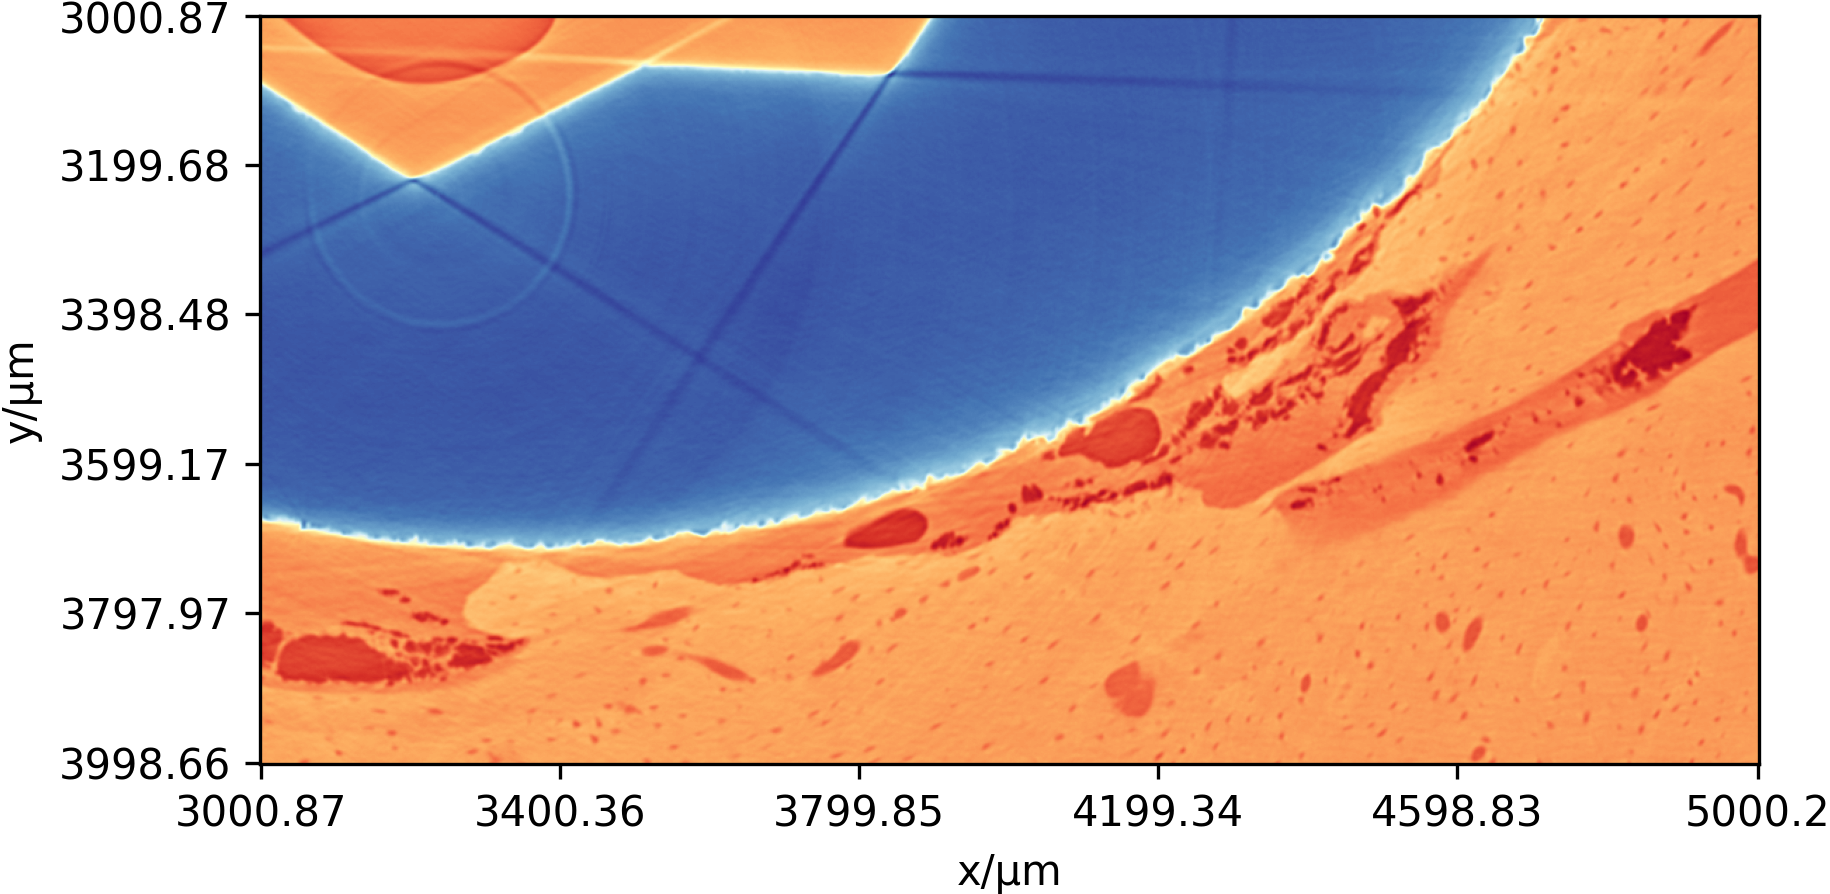
\includegraphics[width=\textwidth]{770c_pag-bic-xy-1x.png}
\caption{Here we see a 1mm x 2mm region of an unscaled image slice in the XY dimension. It highlights
some of the imperfections and noise present in the data. We especially see artifacts within and
around the titanium implant.}
\label{fig:xy-slice}
\end{figure*}

In \cref{fig:xy-slice} and \cref{fig:yz-slice} we see zoomed in regions of the XY and YZ planes
of the same sample as shown in \cref{fig:3viewsample}.

\begin{figure}
\centering
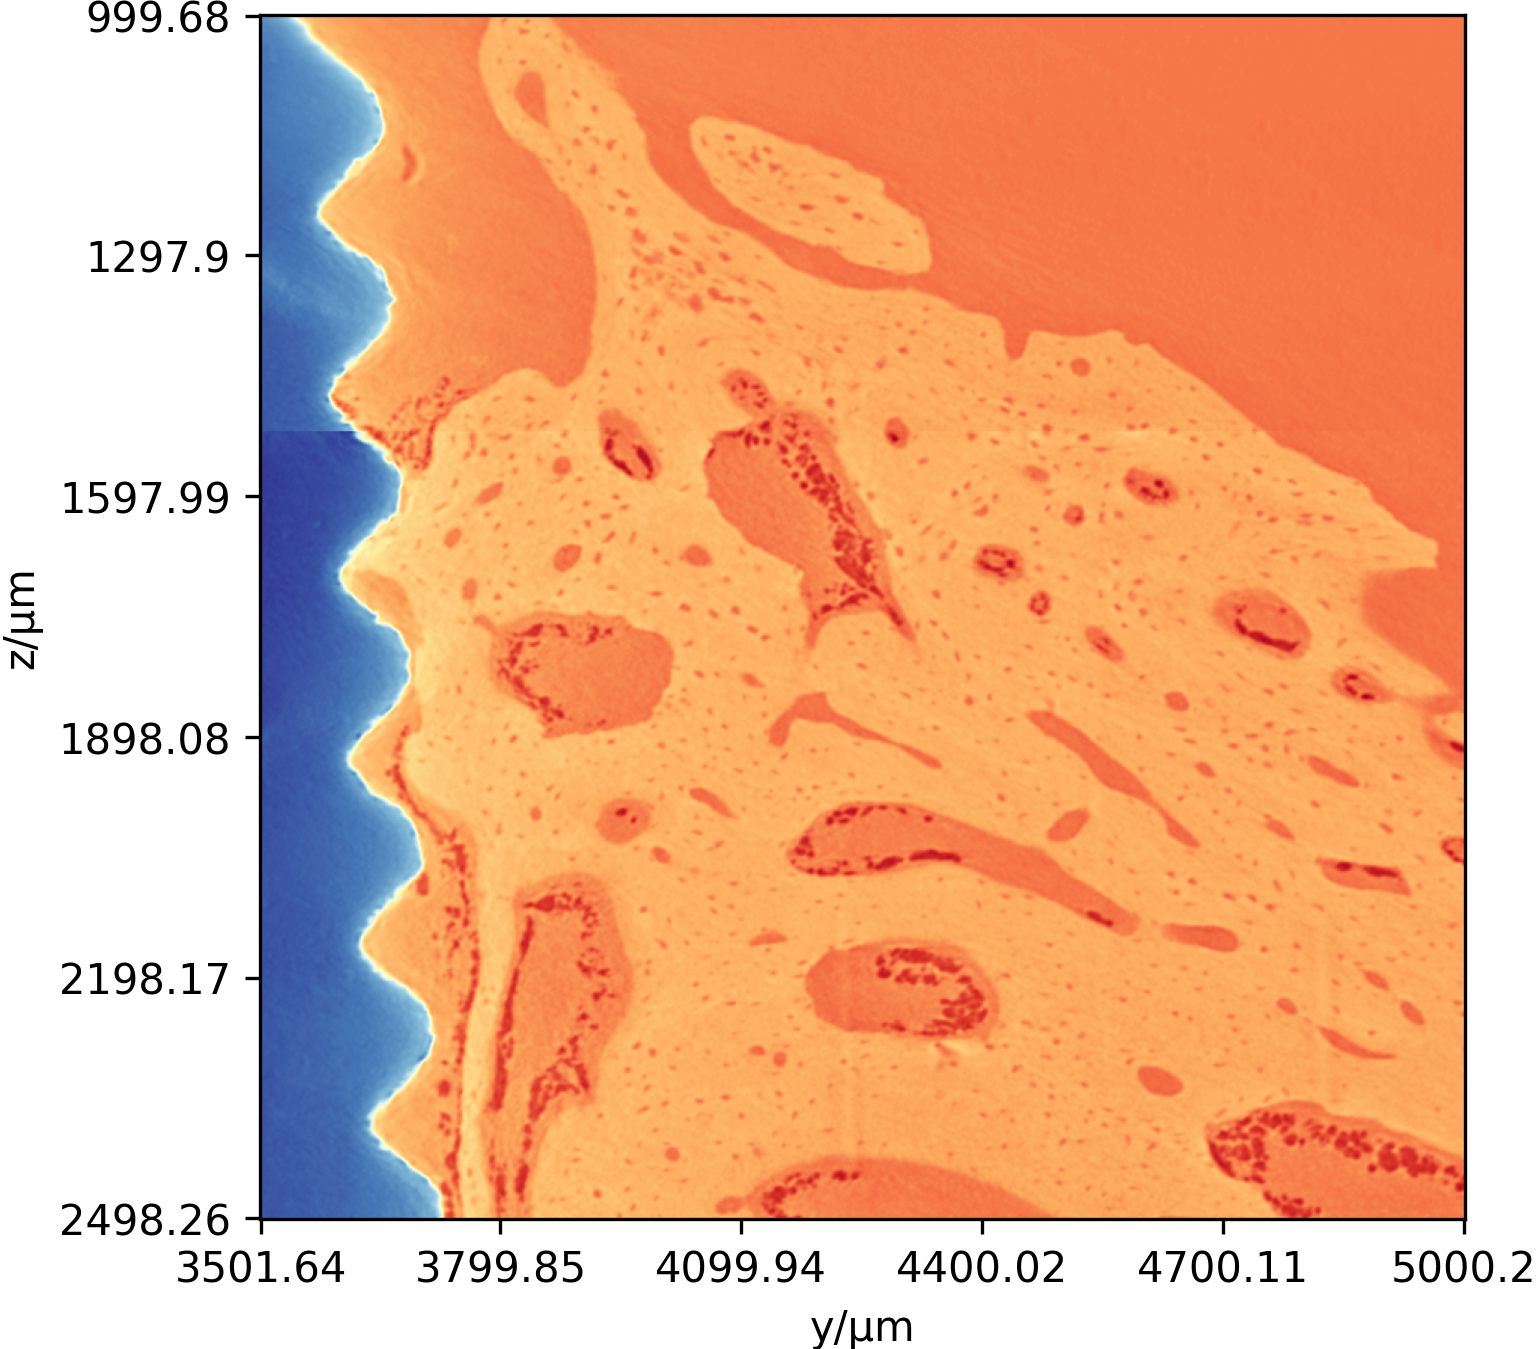
\includegraphics[width=\columnwidth]{770c_pag-bic-yz-1x.png}
\caption{Here we see a 1.5mm x 1.5mm region of an unscaled image slice in the YZ dimension. This
hightlights noise and voxexl effects around the newly formed bone in the micro threaded part of
the titanium implant.}
\label{fig:yz-slice}
\end{figure}

Both planes display a broad selection of the various type of noise sources found in the data.

\subsubsection{Ring artifacts}

Looking at the XY-slice in \cref{fig:xy-slice} we see clear concentric ring artifacts emanating from
the center of the sample, and at strong edges of the titanium implant. It propagates strongly through
the large region of air behind the implant. Compared to the other artifacts mentioned, this effect is
arising from imperfections in the scanner setup. These types of artifacts can typically come from
uncalibrated or defect adjacent detector elements. For synchrotron radiation sources it can also
occur from shifts and vibrations in the monochromator crystal \citep{ringartifacts}.

\subsubsection{Projection artifacts}

Bright streaks with strong edges are seen from the sharp corners of the titanium implant. When
doing back projection, the symmetry breaking is seen as smeared lines across the sample. This
can occur from the high pass filter used during filtered back projection, which exaggerates the
differences between adjacent elements \citep{ctnoise}.

\subsubsection{Compton scattering}

Lower energy rays contribute mostly with noise from scattering effects. A ray will propagate through
a material, get scattered and diffract from its initial trajectory. This gives a misrepresentation
of the attenuation along its initial trajectory. The artefacts seen from scattering are similar in
nature to those formed by beam hardening. This is because both effectively reduce the measured
attenuation. For energy levels of above 50KeV relevant for the data presented here, Compton
scattering is the dominating type \citep{compton}. The scattering occurs due to photon-electron
interaction between X-ray beam and the material it passes through. Like beam-hardening, scattering
will cause dark streaks across the image, where attenuation was highest.

\subsection{Beam hardening}\label{sec:beam-hardening}

Medical CT and $\mu$CT both utilize poly-energetic beams, which can cause artifacts around high
density regions. This effect is called beam-hardening \citep{beamhardening}, and occurs when rays
with lower energy are attenuated more frequently, thus shifting the remaining photon energy to a
higher effective average value. This offsets the local contrast, by overestimating the attenuation,
leaving lighter spots on the image. Many types of artifacts will typically be present in these
setups, but most are taken into account by calibration using phantoms and pre-hardening the beam
before it reaches the sample. Pre-hardening of the beam is done using filters that attenuate the
softest rays. Due to its common usage, various metal artifact reduction (MAR) software exists to
account for noise and imperfections during reconstruction \citep{mar1}\citep{mar2}.

Despite the practially mono-energetic rays from SR$\mu$CT, the source initially generates a
polychromatic spectrum. During monochromatisation the resulting spectrum can still contain
corrupted harmonic components. Only a few percent corruption is enough to produce strong
artifacts, although monochromatisation is typically done in multiple layers \citep{srnoise}.
It can not trivially be rejected that some noise does occur from poly-energetic incident radiation.
Two distinct effects typically seen as a result of beam-hardening are in dark and bright streaks
and cupping artifacts in high density regions.

\subsubsection{Dark and bright streaks}

Streaking artifacts occur at the dense implant region, but also in the transition from bone to softer
tissue. This effect is mostly seen in regions of large heterogeneity. When X-ray beams pass at angles
containing multiple dense obstacles, the beam is hardened more. Then for angles with fewer dense
obstacles the energy spectrum is preserved better. This produced the dark and bright streaks seen in
\cref{fig:xy-slice}.

For a hardened beam, softer x-rays are absorbed instead of successfully penetrating the object,
and will not contribute to image formation. High density structures such as the titanium implant
break the isotropy, making the projected X-ray mean energy spectrum dependent on incident orientation
\citep{srnoise}.

\subsubsection{Cupping effect}

A common artefact that occurs when beams pass more homogeneous cylindrical objects. Since beams
passing the middle will traverse more material compared to the edges, the beam is hardened more
towards the center and intensity becomes lower as a result. This can manifest itself in what
errnoeously looks to be dense peripheral regions at the edges.

\subsection{Phase contrast}

\aleksandar{TODO: Glem ikke denne paragraf!!!}

Phase contrast is an effect whose consequences are not very unlike those of beam-hardening.
Although used as an advantage in holotomography\citep{holotomography} and phase contrast tomography\citep{phasecontrast},
it induces noise in regular tomography such as used here. It typically results in fringes around edges
of regions within the image\citep{srnoise}. Similar to dark and bright streaks mentioned above,
they show as misrepresentations of the voxel values. In our case we see them especially at the
transitional edges between the titanium implant and the biological tissue and bone.

%Partial volume artifacts which are dependent on the voxel size and are mentioned briefly by Neldam et al.

%%% Local Variables:
%%% mode: latex
%%% TeX-master: "main"
%%% End:


\section{Physical effects}
\label{sec:physics}

Noise in tomography is unavoidable, and it makes segmentation harder because it further obscures the
boundaries between materials. Materials may be well separated from certain angles in the
3d-reconstructed image, but can overlap from others. Some noise like that corrected by flat-field
correction is very uniformly distributed across images. Other noise is however very spatially
dependent on its surrounding regions. Knowing the composition and positioning of the materials being
imaged, we can counter some of these effects during segmentation. The effects from noise manifest
themselves as numerical shifts in voxel-values as a function of their position. This is a direct
result of a misrepresented attenuation along the axis the X-rays are passing.

This dependency on orientation illustrates how voxel intensity values are not globally fixed.
Instead, how a certain material is represented in intensity, is highly dependent on its position
relative to neighbouring regions. Especially since this also determines the amount and type of
derived noise.  The same material with the same density, can thus be represented at multiple varying
intensities within the same sample.

% \begin{figure*} \centering 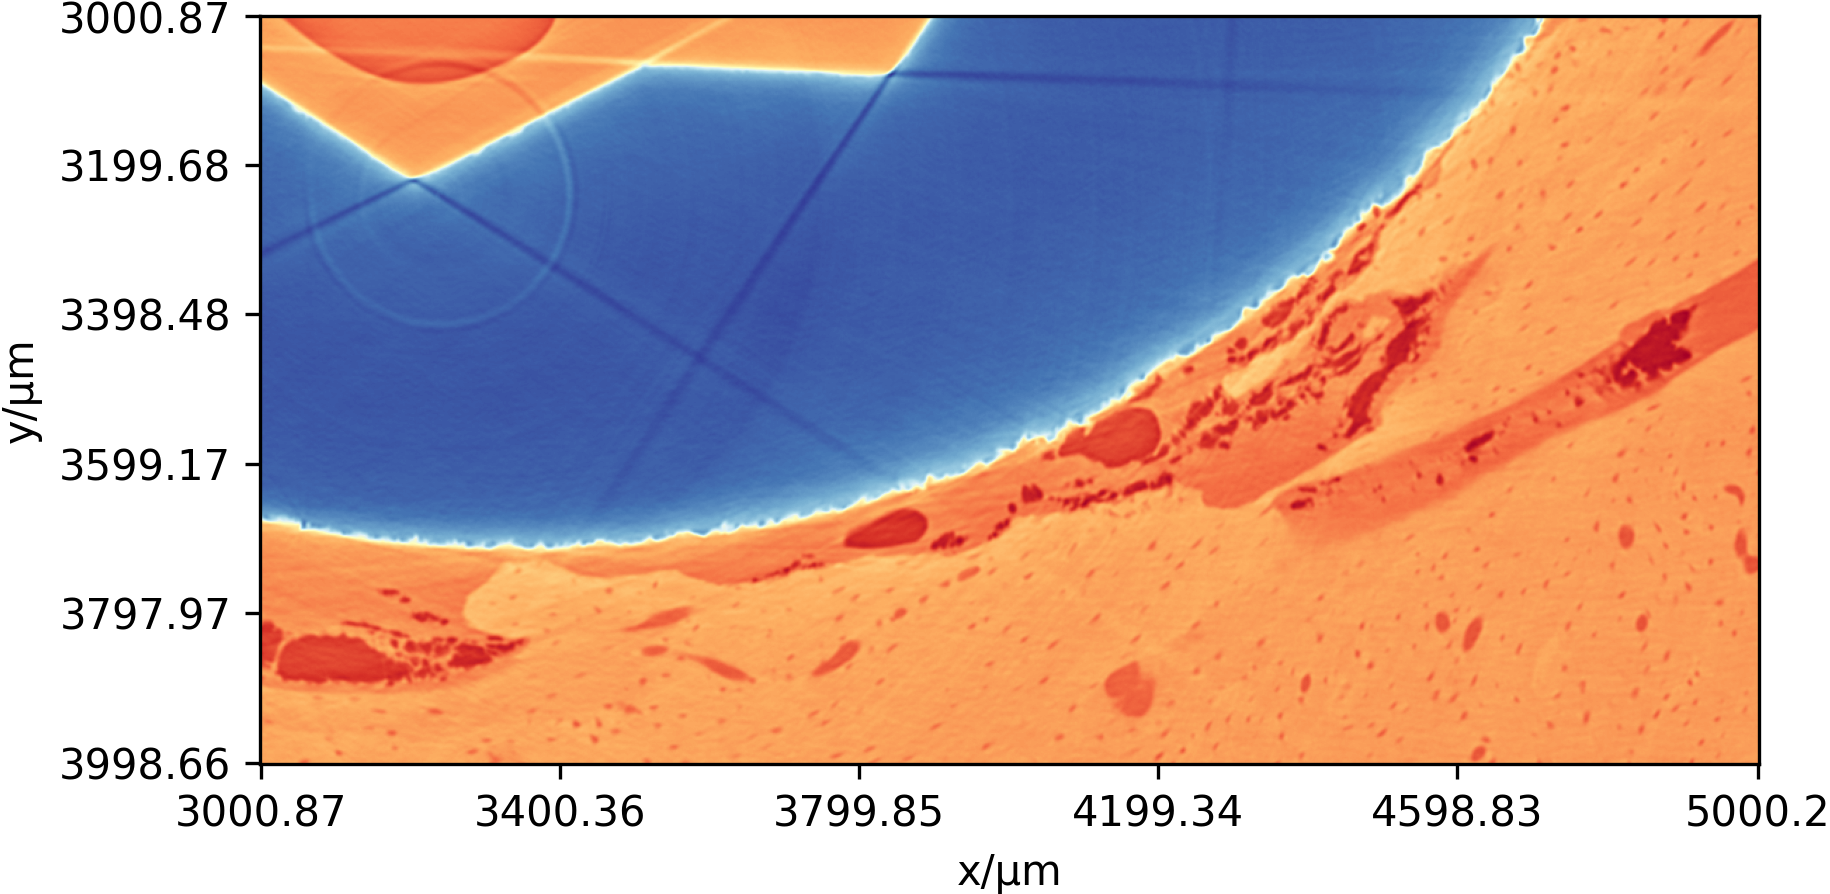
\includegraphics[width=\textwidth]{770c_pag-bic-xy-1x.png}
% \caption{Here we see a 1mm x 2mm region of an unscaled image slice in the XY dimension. It
% highlights some of the imperfections and noise present in the data. We especially see artifacts
% within and around the titanium implant.} \label{fig:xy-slice} \end{figure*}

\begin{figure}
  \centering
  \begin{tabular}{cc}
    \!\!\!\!\!\!(a)\!\!\!&\begin{tabular}{c}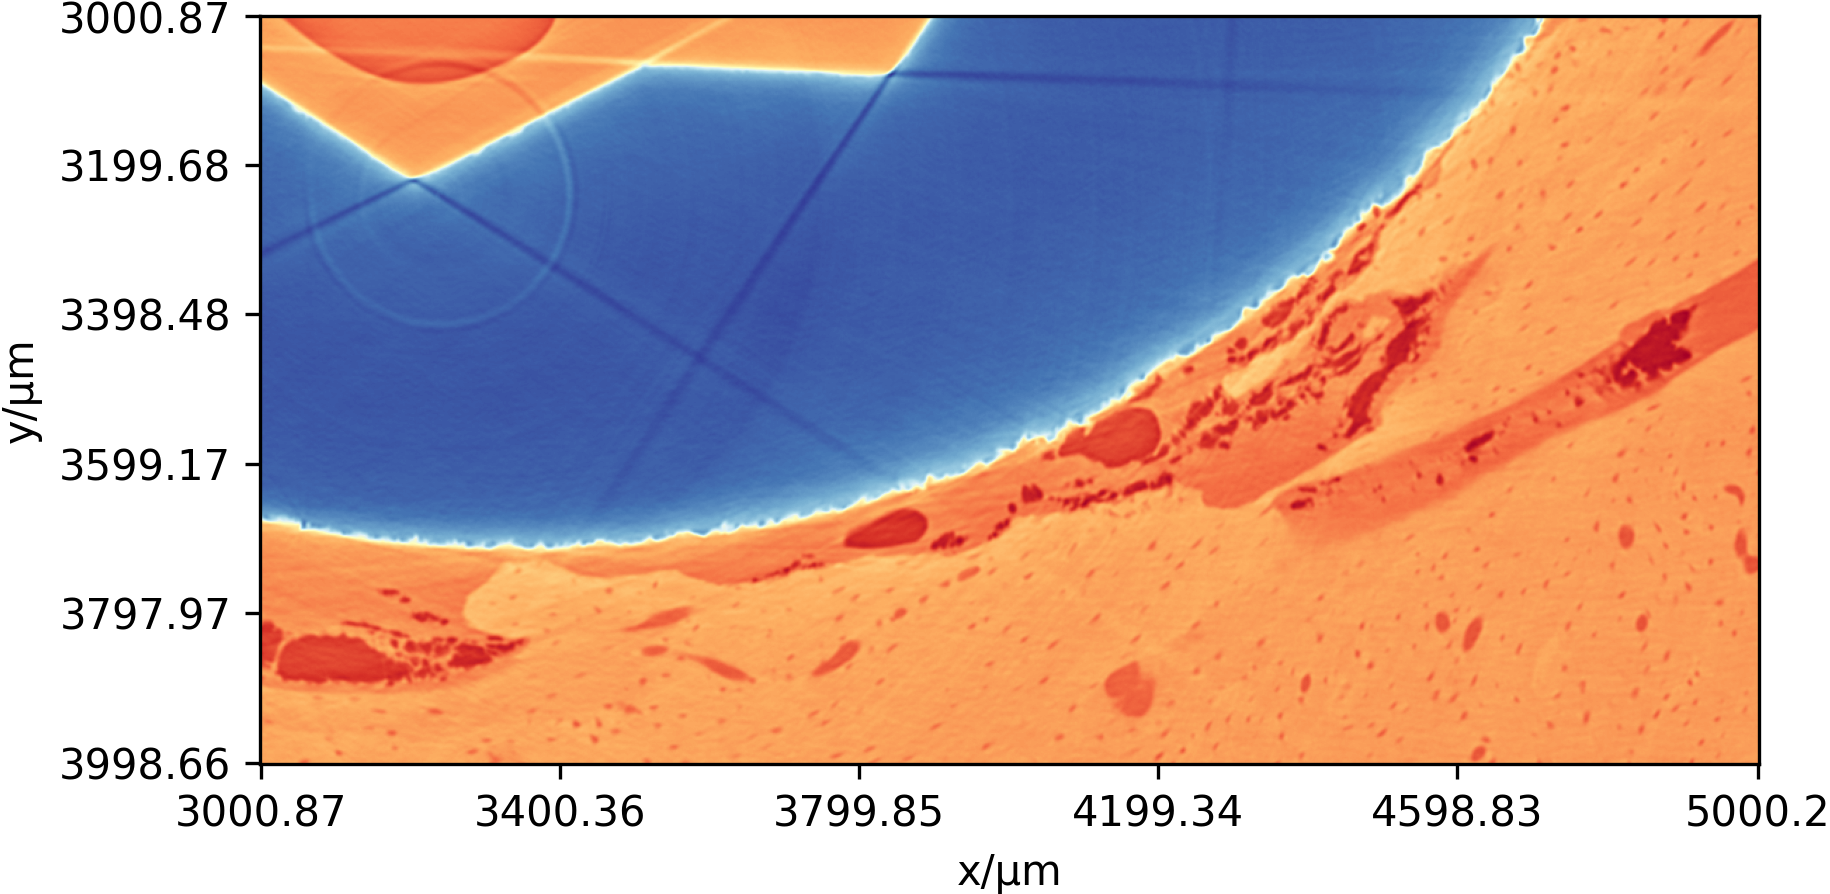
\includegraphics[width=0.96\columnwidth]{770c_pag-bic-xy-1x.png}\end{tabular}\\
    \!\!\!\!\!\!(b)\!\!\!&\begin{tabular}{c}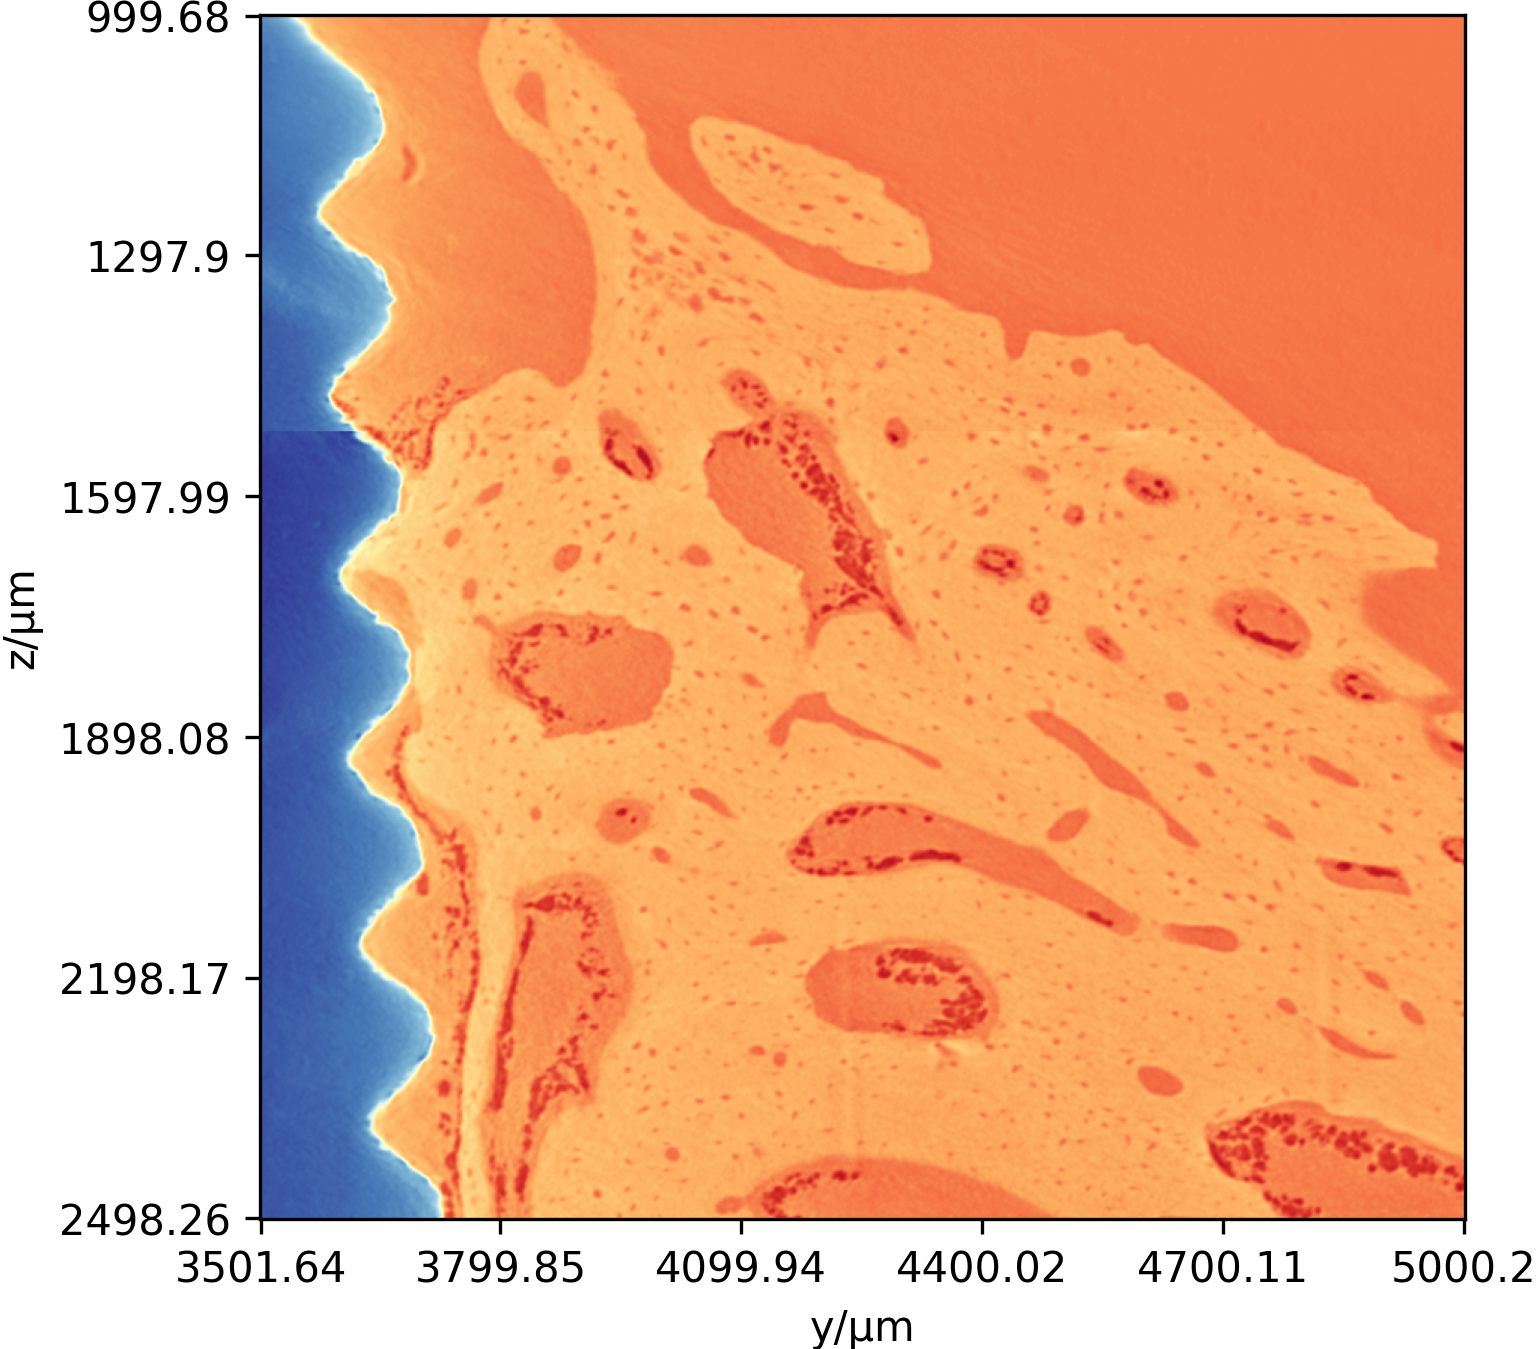
\includegraphics[width=0.96\columnwidth]{770c_pag-bic-yz-1x.png}\end{tabular}\\    
  \end{tabular}
  \caption{
    To better see the distortion effects, we zoom in on sub-regions of the slices shown in
    \Cref{fig:3viewsample}. Our visual systems automatically correct for most of the distortions,
    as they appear similar to illumination effects. However, even some distance from the implant,
    blood vessel voxels have higher values than bone voxels further out. As we approach the implant,
    the value-shifts accelerates and becomes highly non-linear.
    (a) A 1mm$\times$2mm region of an image slice in the XY-plane.
    % It highlights some of the imperfections and noise present in the data.
    (b) A 1.5mm x 1.5mm region of an image slice in the YZ-plane in the micro threaded part of
    the titanium implant.
  }
\label{fig:slices}
\end{figure}

In \Cref{fig:slices}, we see zoomed in regions of the XY- and YZ-planes of the same sample as shown
in \Cref{fig:3viewsample}.  Both planes display a broad selection of the various type of noise
sources found in the data.

\paragraph{Beam hardening}
Medical CT and $\mu$CT both utilize poly-energetic beams, which can cause artefacts around high
density regions. This effect is called beam-hardening \citep{beam-hardening}, and occurs when rays
with lower energy are attenuated more frequently, thus shifting the remaining photon energy to a
higher effective average value. This offsets the local contrast, by overestimating the attenuation,
leaving lighter spots on the image. Many types of artefacts will typically be present in X-ray 
setups, but most are taken into account by calibration using phantoms and pre-hardening the beam
before it reaches the sample. Pre-hardening of the beam is done using filters that attenuate the
softest rays. Due to its common usage, various metal artefact reduction (MAR) software exists to
account for noise and imperfections during reconstruction \citep{mar1}\citep{mar2}.

Despite the practically mono-energetic rays from SR$\mu$CT, the source initially generates a
poly-chromatic spectrum. During monochromatisation the resulting spectrum can still contain
corrupted harmonic components. Only a few percent corruption is enough to produce strong artefacts,
although monochromatisation is typically done in multiple layers \citep{srnoise}.  It can not
trivially be rejected that some noise does occur from poly-energetic incident radiation.  Two
distinct effects typically seen as a result of beam-hardening are in dark and bright streaks and
cupping artefacts in high density regions.

\paragraph{Dark and bright streaks} Streaking artefacts occur at the dense implant region, but also
in the transition from bone to softer tissue. This effect is mostly seen in regions of large
heterogeneity. When X-ray beams pass at angles containing multiple dense obstacles, the beam is
hardened more. Then for angles with fewer dense obstacles the energy spectrum is preserved better.
This produced the dark and bright streaks seen in \Cref{fig:slices}.

For a hardened beam, softer x-rays are absorbed instead of successfully penetrating the object, and
will not contribute to image formation. High density structures such as the titanium implant break
the isotropy, making the projected X-ray mean energy spectrum dependent on incident orientation
\citep{srnoise}.

\paragraph{Cupping effect} A common artefact that occurs when beams pass more homogeneous
cylindrical objects. Since beams passing the middle will traverse more material compared to the
edges, the beam is hardened more towards the center and intensity becomes lower as a result. This
can manifest itself in what erroneously looks to be dense peripheral regions at the edges.

\paragraph{Phase contrast} Phase contrast is an effect whose consequences are not very unlike those
of beam-hardening.  Although used as an advantage in holotomography\citep{holotomography} and phase
contrast tomography\citep{phasecontrast}, it induces noise in regular tomography such as used here.
It typically results in fringes around edges of regions within the image\citep{srnoise}. Similar to
dark and bright streaks mentioned above, they show as misrepresentations of the voxel values. In our
case we see them especially at the transitional edges between the titanium implant and the
biological tissue and bone.

\subsection{Other noise and artifacts}
\label{sec:noise-artefacts}

\paragraph{Ring artefacts} Looking at the XY-place in \Cref{fig:slices} we see clear concentric ring
artefacts emanating from the center of the sample, and at strong edges of the titanium implant. It
propagates strongly through the large region of air behind the implant. Compared to the other
artefacts mentioned, this effect is arising from imperfections in the scanner setup. These types of
artefacts can typically come from uncalibrated or defect adjacent detector elements. For synchrotron
radiation sources it can also occur from shifts and vibrations in the monochromator crystal
\citep{ringartefacts}.

\paragraph{Projection artefacts} Bright streaks with strong edges are seen from the sharp corners of
the titanium implant. When doing back projection, a symmetry break is seen as smeared lines across
the sample. This can occur from the high pass filter used during filtered back projection, which
exaggerates the differences between adjacent elements \citep{ctnoise}.

\paragraph{Compton scattering} Lower energy rays contribute mostly with noise from scattering
effects. A ray will propagate through a material, get scattered and diffract from its initial
trajectory. This gives a misrepresentation of the attenuation along its initial trajectory. The
artefacts seen from scattering are similar in nature to those formed by beam hardening. This is
because both phenomena effectively reduce the measured attenuation. For energy levels relevant for
the data presented here, of 50 KeV and above, Compton scattering is the dominant type
\citep{Compton}.  The scattering occurs due to photon-electron interaction between X-ray beam and
the material it passes through. Like beam-hardening, scattering will cause dark streaks across the
image, where attenuation was highest.

\subsection{Dealing with artefacts}
\label{sec:dealwithit}

The distortions that come from the class of physical effects and noise artefacts discussed in this
section, will vary continously as a function of the spatial coordinates. This allows the possibility
for a method, which can correctly identify materials despite varying voxel values.
% FIXME: Would like a reference for the continous argument
% It is also mentioned in the last sentences of the first paragraph in
% "Physical effects, noise and artifacts"

%Partial volume artefacts which are dependent on the voxel size and are mentioned briefly by Neldam et al.


%%% Local Variables:
%%% mode: latex
%%% TeX-master: "main"
%%% End:


\section{Method}\label{sec:method}
% Spatial correlation 2d histograms (den nemme, 1 2d hist)
In this section, we will describe the method for exploiting spatial correlation based on the
2D-histograms of the tomographies. We will start by motivating the problem, then give an overview
of how we solve the problem, with a final detailed walkthrough of each step in the overall workflow.

\subsection{1-dimensional histograms}
%diskuter overlappende materialer
Looking at a 1D-histogram of the voxel value in a tomography, as shown in~\Cref{fig:1d-hist}, we are
able to distinguish different distributions, but we see that there is a large overlap. This leads to
global thresholding being infeasible, at least for the distributions in the lower half of the histogram.
This happens because the voxel value is not globally defined, as~\Cref{sec:physics} explains, which
illustrates how the different materials cover ranges of values that blend together in the histogram.

\begin{figure}
    \centering
    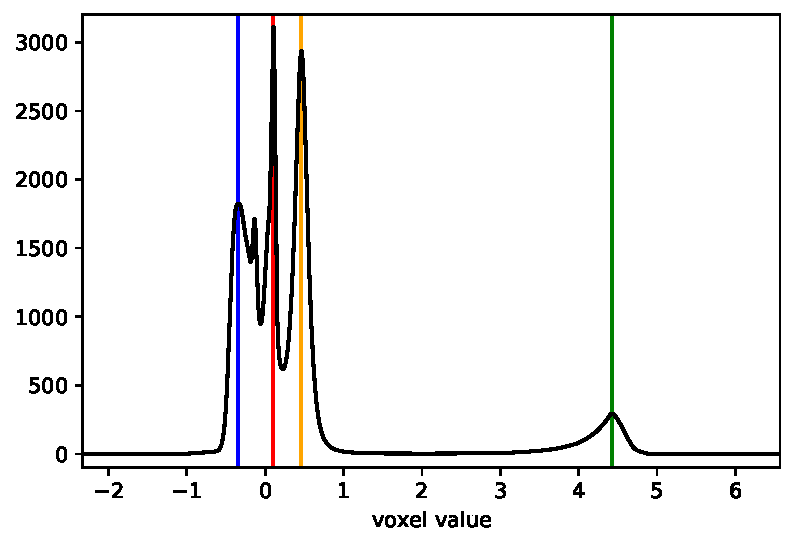
\includegraphics[width=\linewidth]{1d_hist.pdf}
    \caption{1-dimensional histogram of the voxel values of a tomography. The blue line is air peak,
    the red line is the soft tissue peak, the green line is the bone peak, and the orange line is
    the implant peak.}
    \label{fig:1d-hist}
\end{figure}

\subsection{Preprocessing}\label{sec:preprocess}
To reduce the complexity of the segmentation process, we preprocess the data by removing redundant
information. From our work in an upcoming paper under preparation, we are able to obtain two
masks: an \textit{implant mask} and a \textit{bone mask}.

Since the values of the implant material is radically different from the rest of the sample, obtaining
the rough implant mask through global thresholding is trivial, as the orange line in~\Cref{fig:1d-hist}
shows. This mask is then refined, along with the internal gaps being closed, giving us the implant mask.
Using this mask, we are also able to remove the air making up half of the sample cylinder. This is depicted
in~\Cref{fig:3viewsample}, above the implant and to the left of the implant in the XY and YZ cross
sections respectively. Finally the implant mask can show us the orientation of the implant. This squashes
the blue peak from the histogram, leaving the two peaks marked by the red and green lines as being
the most defined.

As we are only interested in the voxels inside the bone, and we know that bone is the most prominent
material left, we perform another coarse segmentation. This is done by thresholding between the two
large distributions, choosing everything to the right of this threshold as the bone mask. These voxels
are morphologically closed, to also consumes the internal gaps in the bone region, which makes up the
soft tissue inside the bone. The implant and bone region masks are applied throughout subsequent steps
to filter out noise in the tomography.

\subsection{Exploiting spatial information}
% Show the correlation of x,y,z,r to histograms 2d
As described in~\Cref{sec:physics}, the voxel values vary according to their positioning, motivating
us to utilize spatial information in the tomography. In order to include spatial information,
we consider \textit{expanding} a dimension to produce multiple 1D histograms into a combined 2-dimensional
histogram. Each 2D histogram is computed by locking the dimension in question and produce the 1D histograms.
Specifically, we consider the radius ($r$) dimension from the center of the implant, as the voxel values
vary most, closest to the implant. The algorithm for computing the 2-dimensional histogram for the
radius can be seen in~\Cref{alg:2dhists} with the resulting 2D histogram plotted in~\Cref{fig:2dhists}.
From this plot, we see two prominent distributions that change along the $r$ axis. This is however
not an accurate representation, as the edges of the implant are not uniformly spread across the longest
axis of the implant. This means that the radius does not sufficiently represent the distance from the
implant at high resolutions. This is shown in~\Cref{fig:edt-vs-diffusion}, where we see that a radius
of constant value from the center has varying distance to the implant.

% Kept for historical reasons.
%\begin{algorithm}
%    \caption{2-dimensional histograms. Allocation also implies zero initialization.}
%    \label{alg:2dhists}
%    \begin{algorithmic}
%        \Function {2D\_hist} {$voxels[n_z,n_y,n_x],c_x,c_y,n_{bins},v_{min},v_{max}$}
%            \State $n_r \gets \left\lfloor\sqrt{\left\lfloor \frac{n_x}{2} \right\rfloor^2 + \left\lfloor \frac{n_y}{2} \right\rfloor^2}\right\rfloor+1$
%            \State \textbf{allocate} $h_z[n_z,n_{bins}], h_y[n_y,n_{bins}]$
%            \State \textbf{allocate} $h_x[n_x,n_{bins}], h_r[n_r,n_{bins}]$
%            \For {$z,y,x$ \textbf{in} $0{:}n_z,0{:}n_y,0{:}n_x$}
%                \State $v \gets voxels[z,y,x]$
%                \If {$v_{min} \leq v \leq v_{max}$}
%                    \State $v_{i} \gets (n_{bins}-1) \cdot \frac{v - v_{min}}{v_{max} - v_{min}}$
%                    \State $r \gets \left\lfloor\sqrt{(x-c_x)^2 + (y-c_y)^2}\right\rfloor$
%                    \State $h_z[z,v_{i}]{+}{+}$
%                    \State $h_y[y,v_{i}]{+}{+}$
%                    \State $h_x[x,v_{i}]{+}{+}$
%                    \State $h_r[r,v_{i}]{+}{+}$
%                \EndIf
%            \EndFor
%            \Return $h_z,h_y,h_z,h_r$
%        \EndFunction
%    \end{algorithmic}
%\end{algorithm}

\begin{algorithm}
    \caption{2-dimensional radius histogram.}
    \label{alg:2dhists}
    \begin{algorithmic}
        \Function {hist\_r} {$voxels[n_z,n_y,n_x],c_x,c_y,n_{bins},v_{min},v_{max}$}
            \For {$z,y,x$ \textbf{in} $0{:}n_z,0{:}n_y,0{:}n_x$}
                \State $v \gets voxels[z,y,x]$
                \If {$v_{min} \leq v \leq v_{max}$}
                    \State $v_{i} \gets (n_{bins}-1) \cdot \frac{v - v_{min}}{v_{max} - v_{min}}$
                    \State $r \gets \left\lfloor\sqrt{(x-c_x)^2 + (y-c_y)^2}\right\rfloor$
                    \State $h_r[r,v_{i}]{+}{+}$
                \EndIf
            \EndFor
            \Return $h_r$
        \EndFunction
    \end{algorithmic}
\end{algorithm}

\begin{figure}
    \centering
    %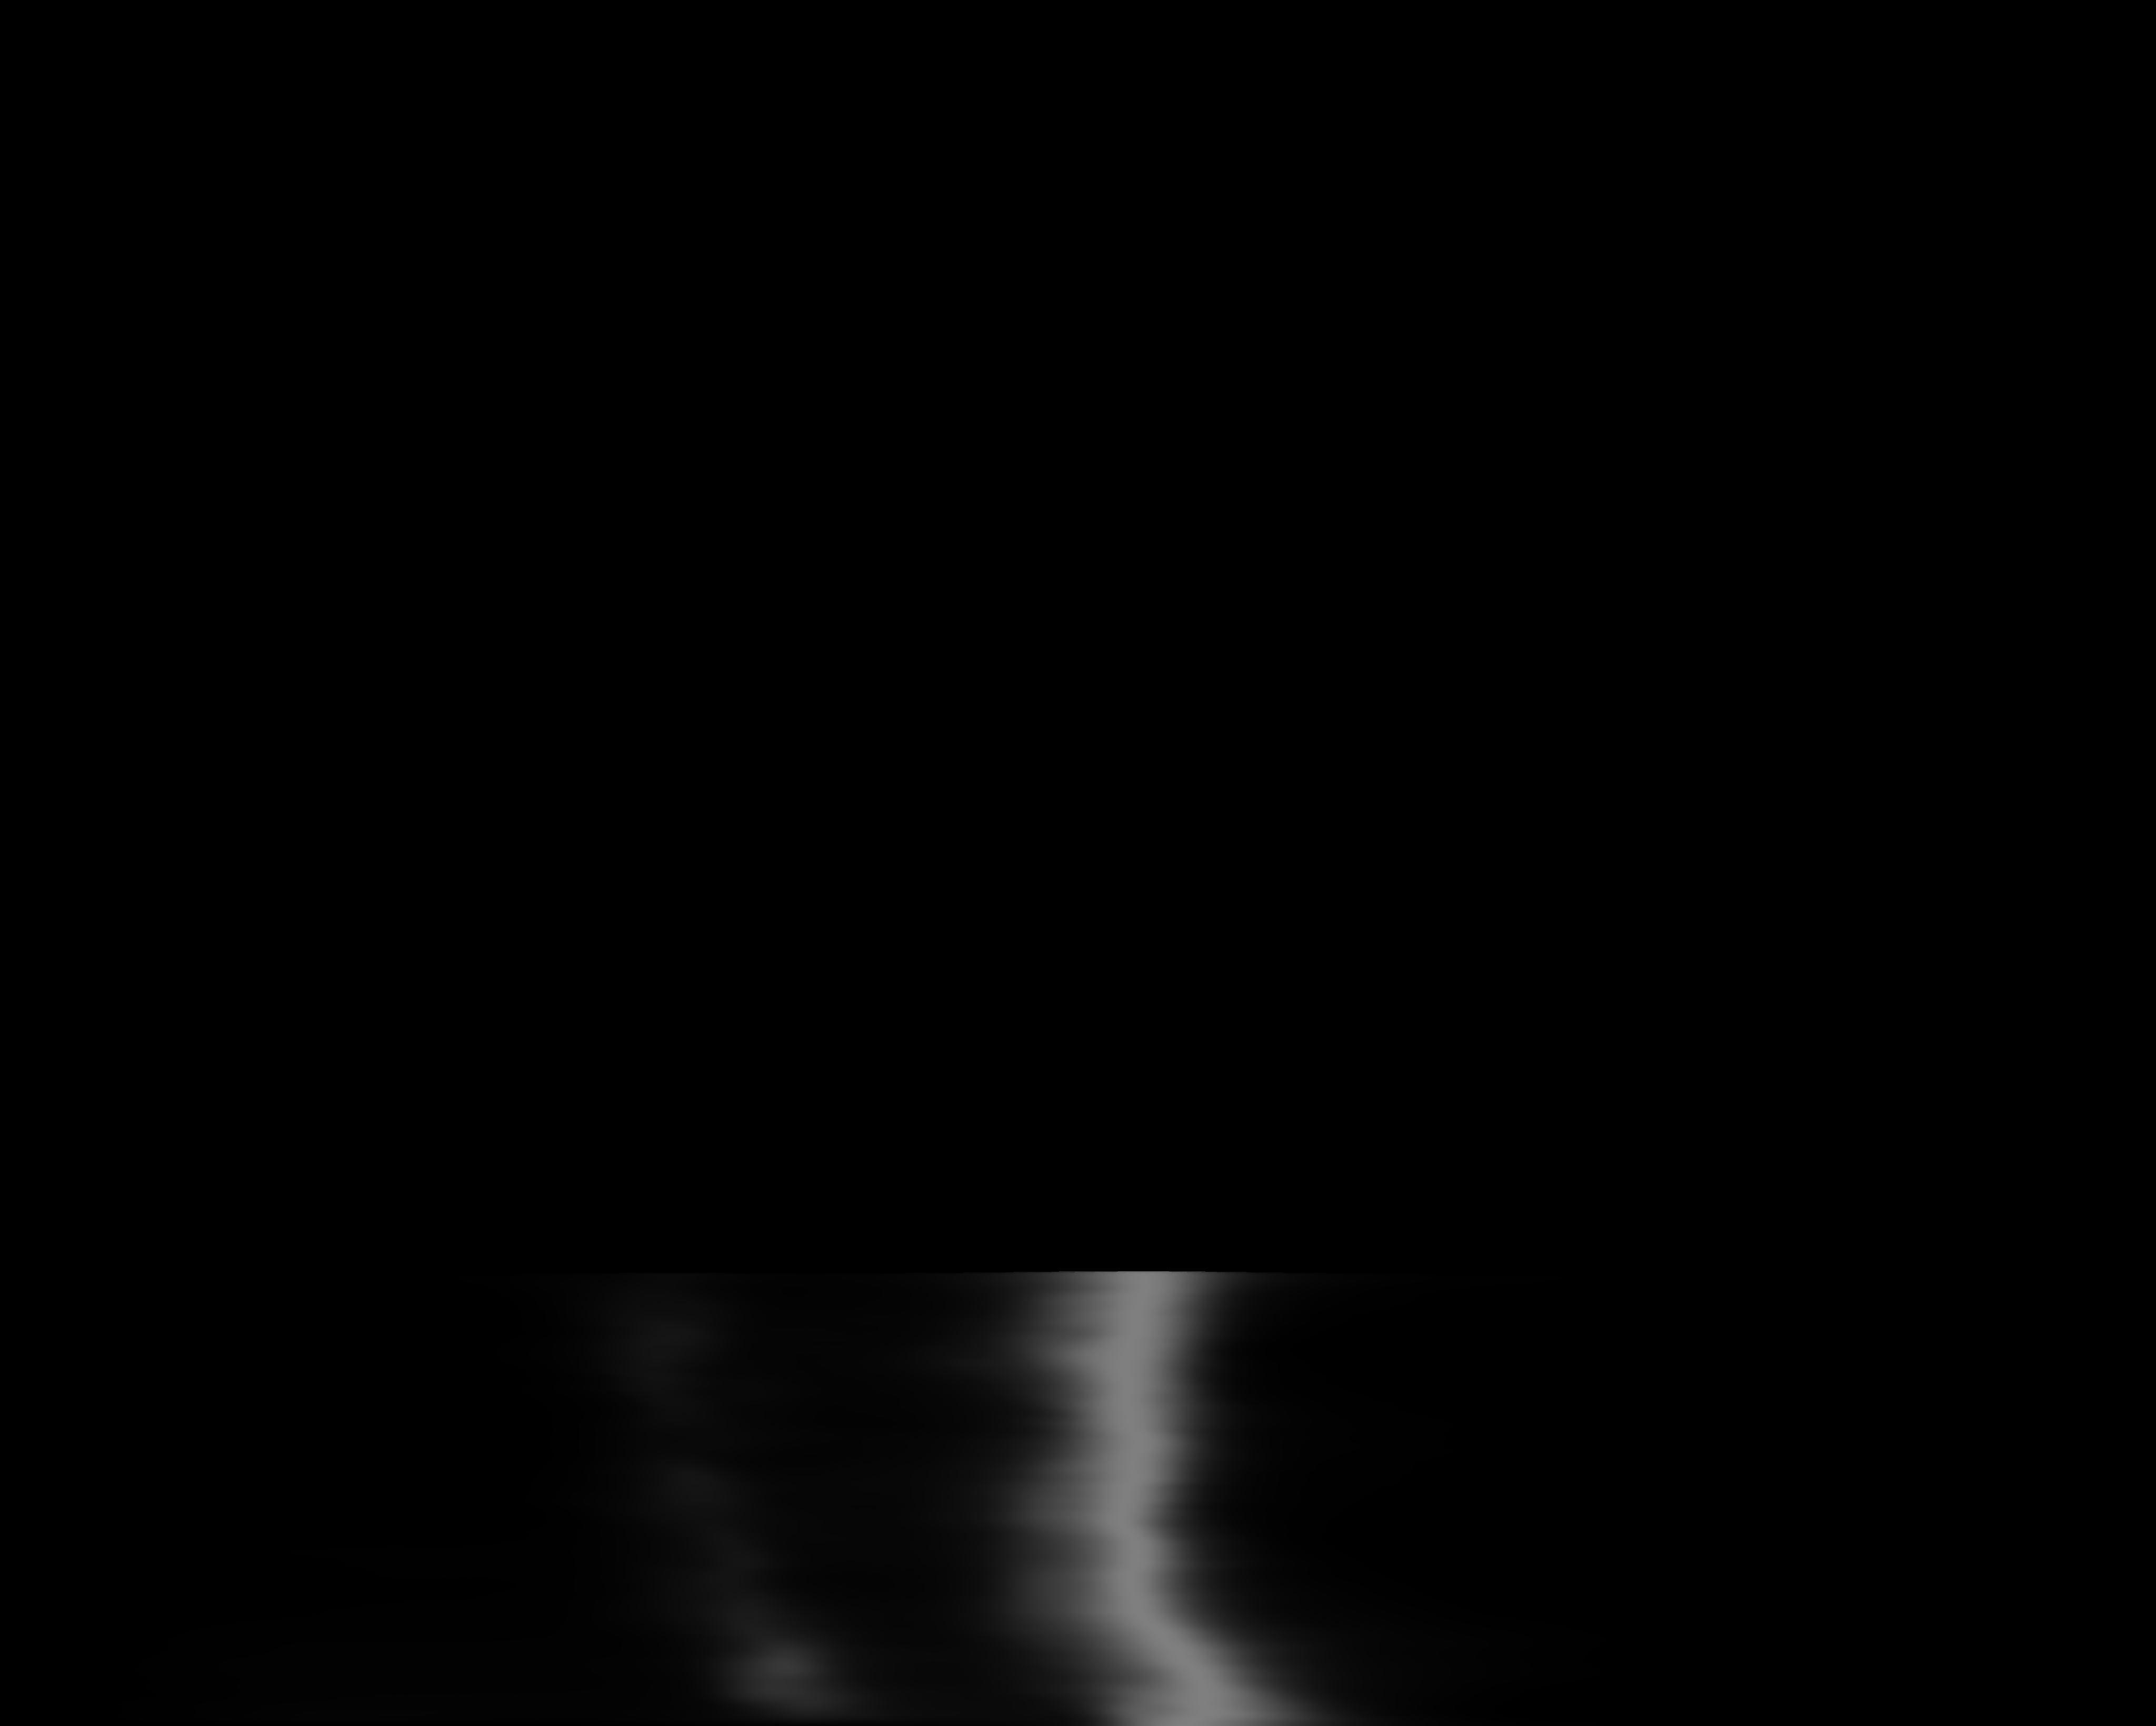
\includegraphics[width=.49\linewidth]{zb-bone_region3.png}
    %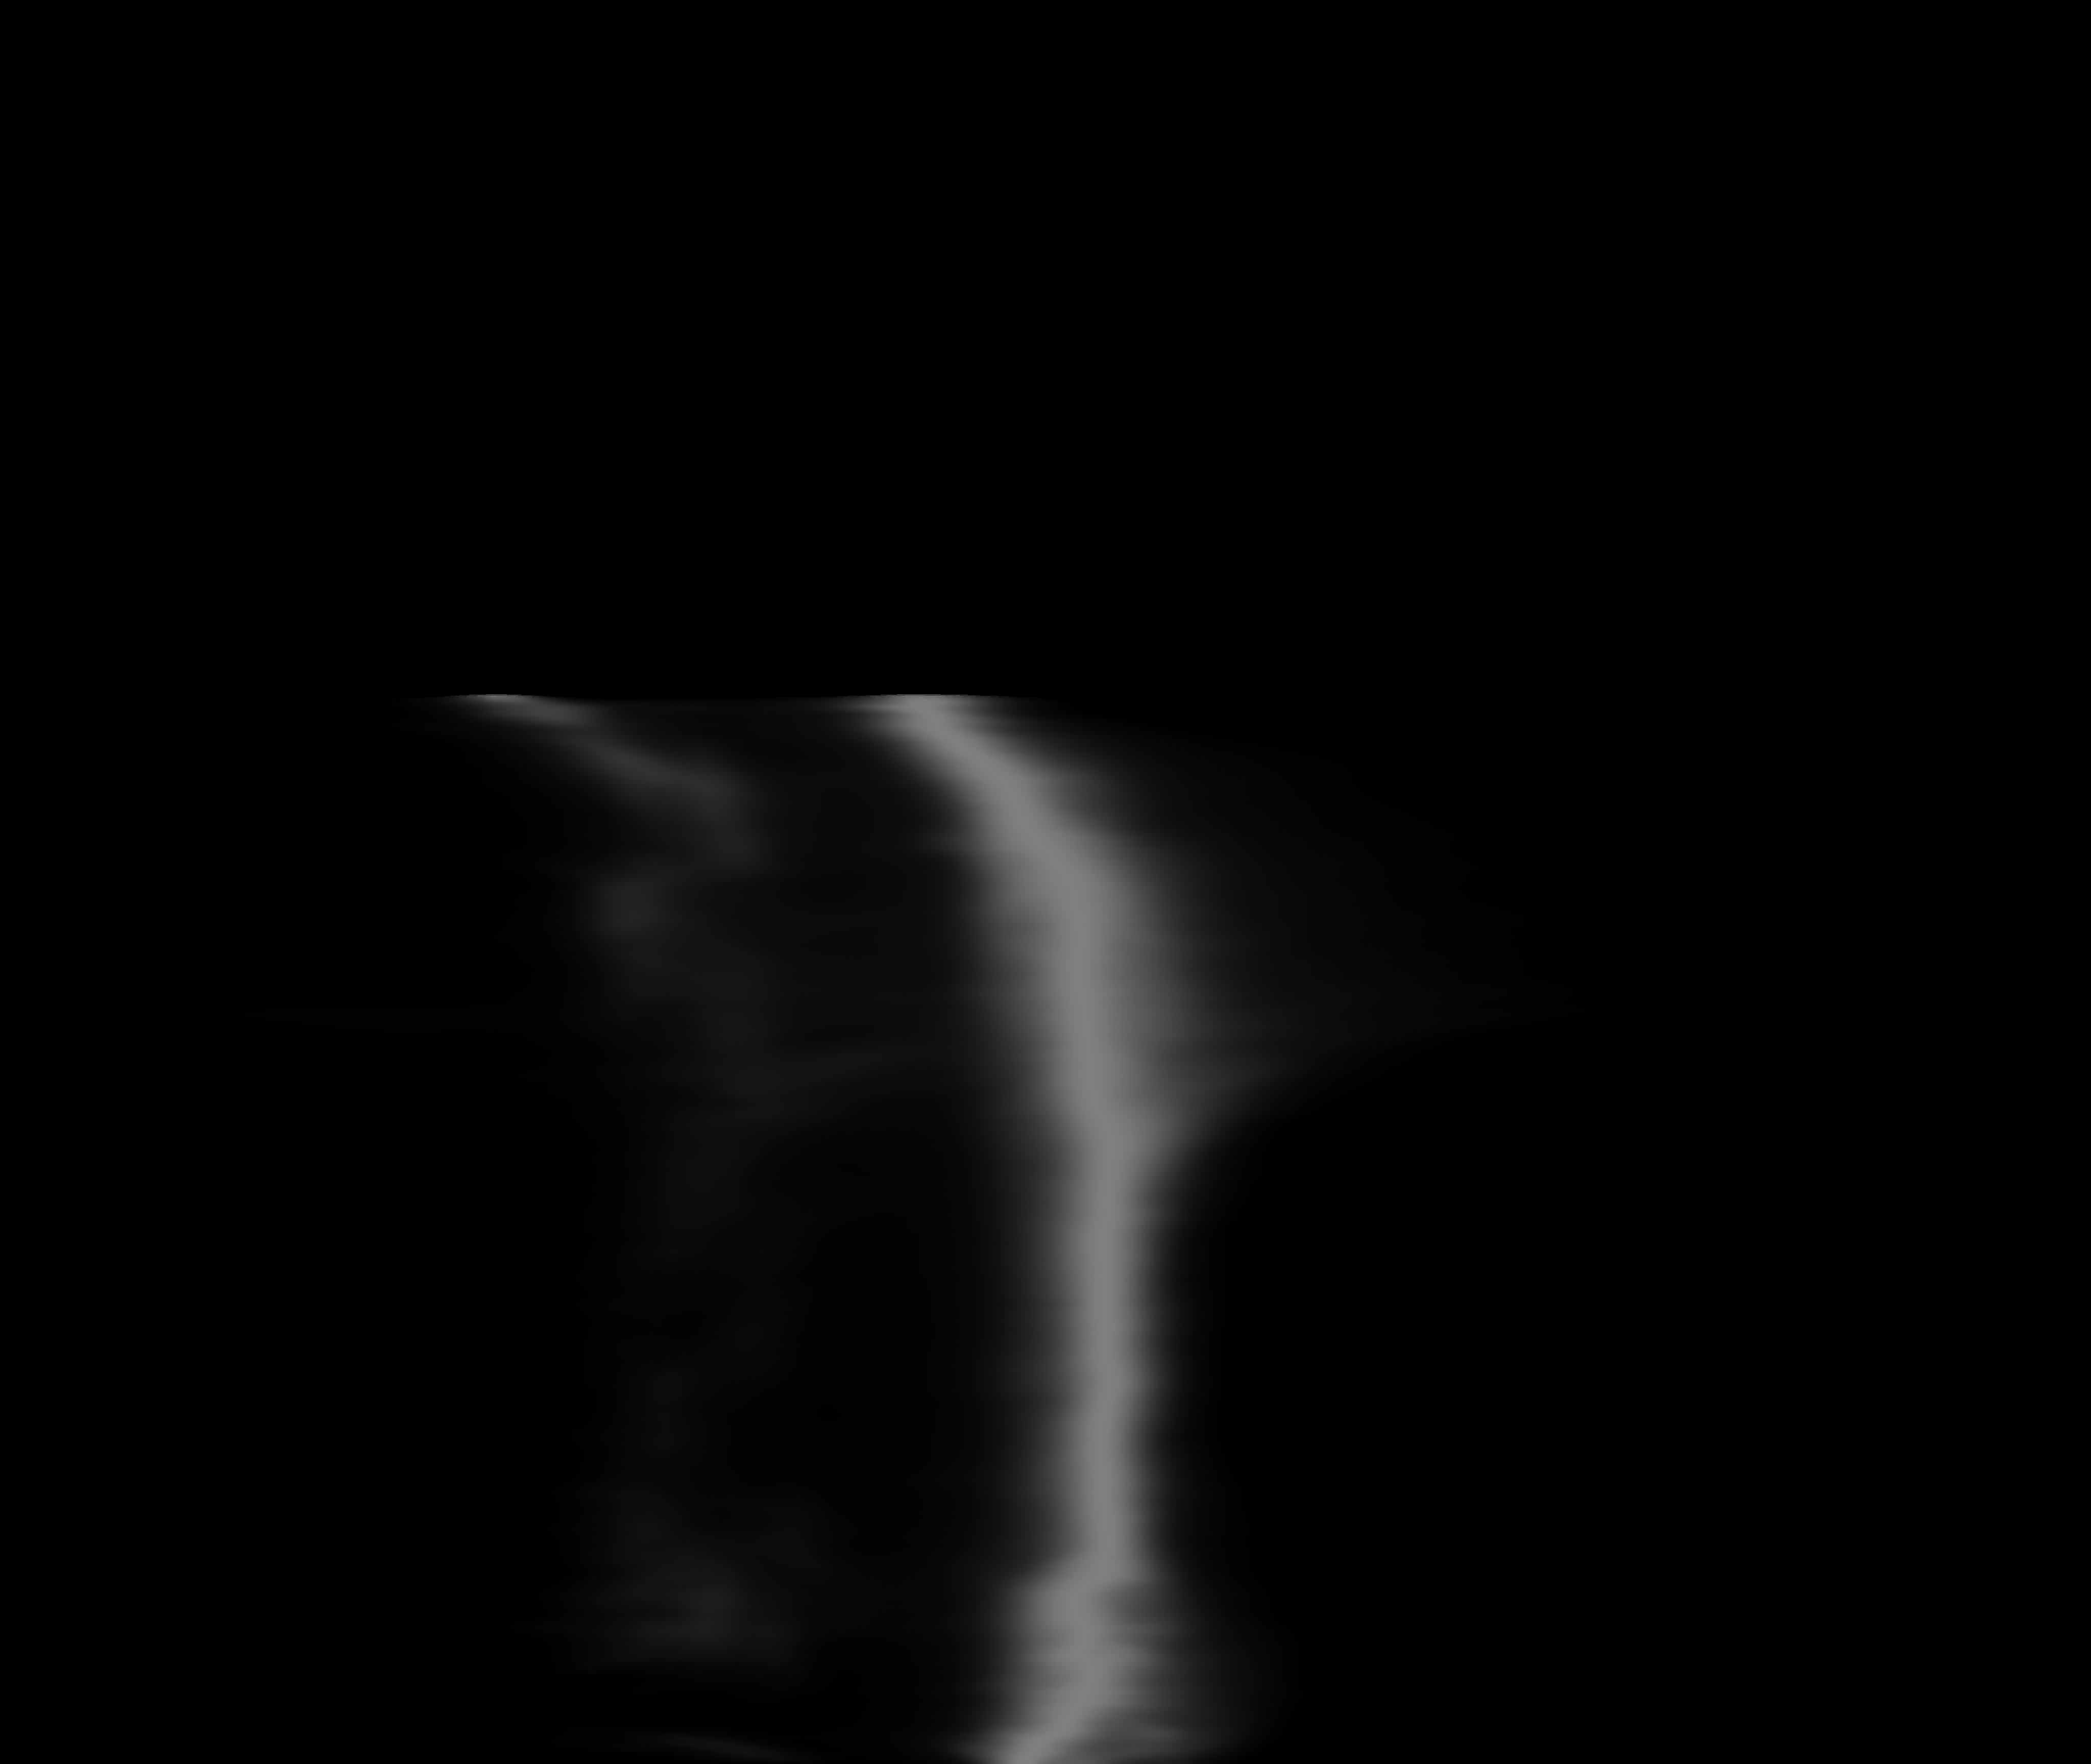
\includegraphics[width=.49\linewidth]{yb-bone_region3.png}
    %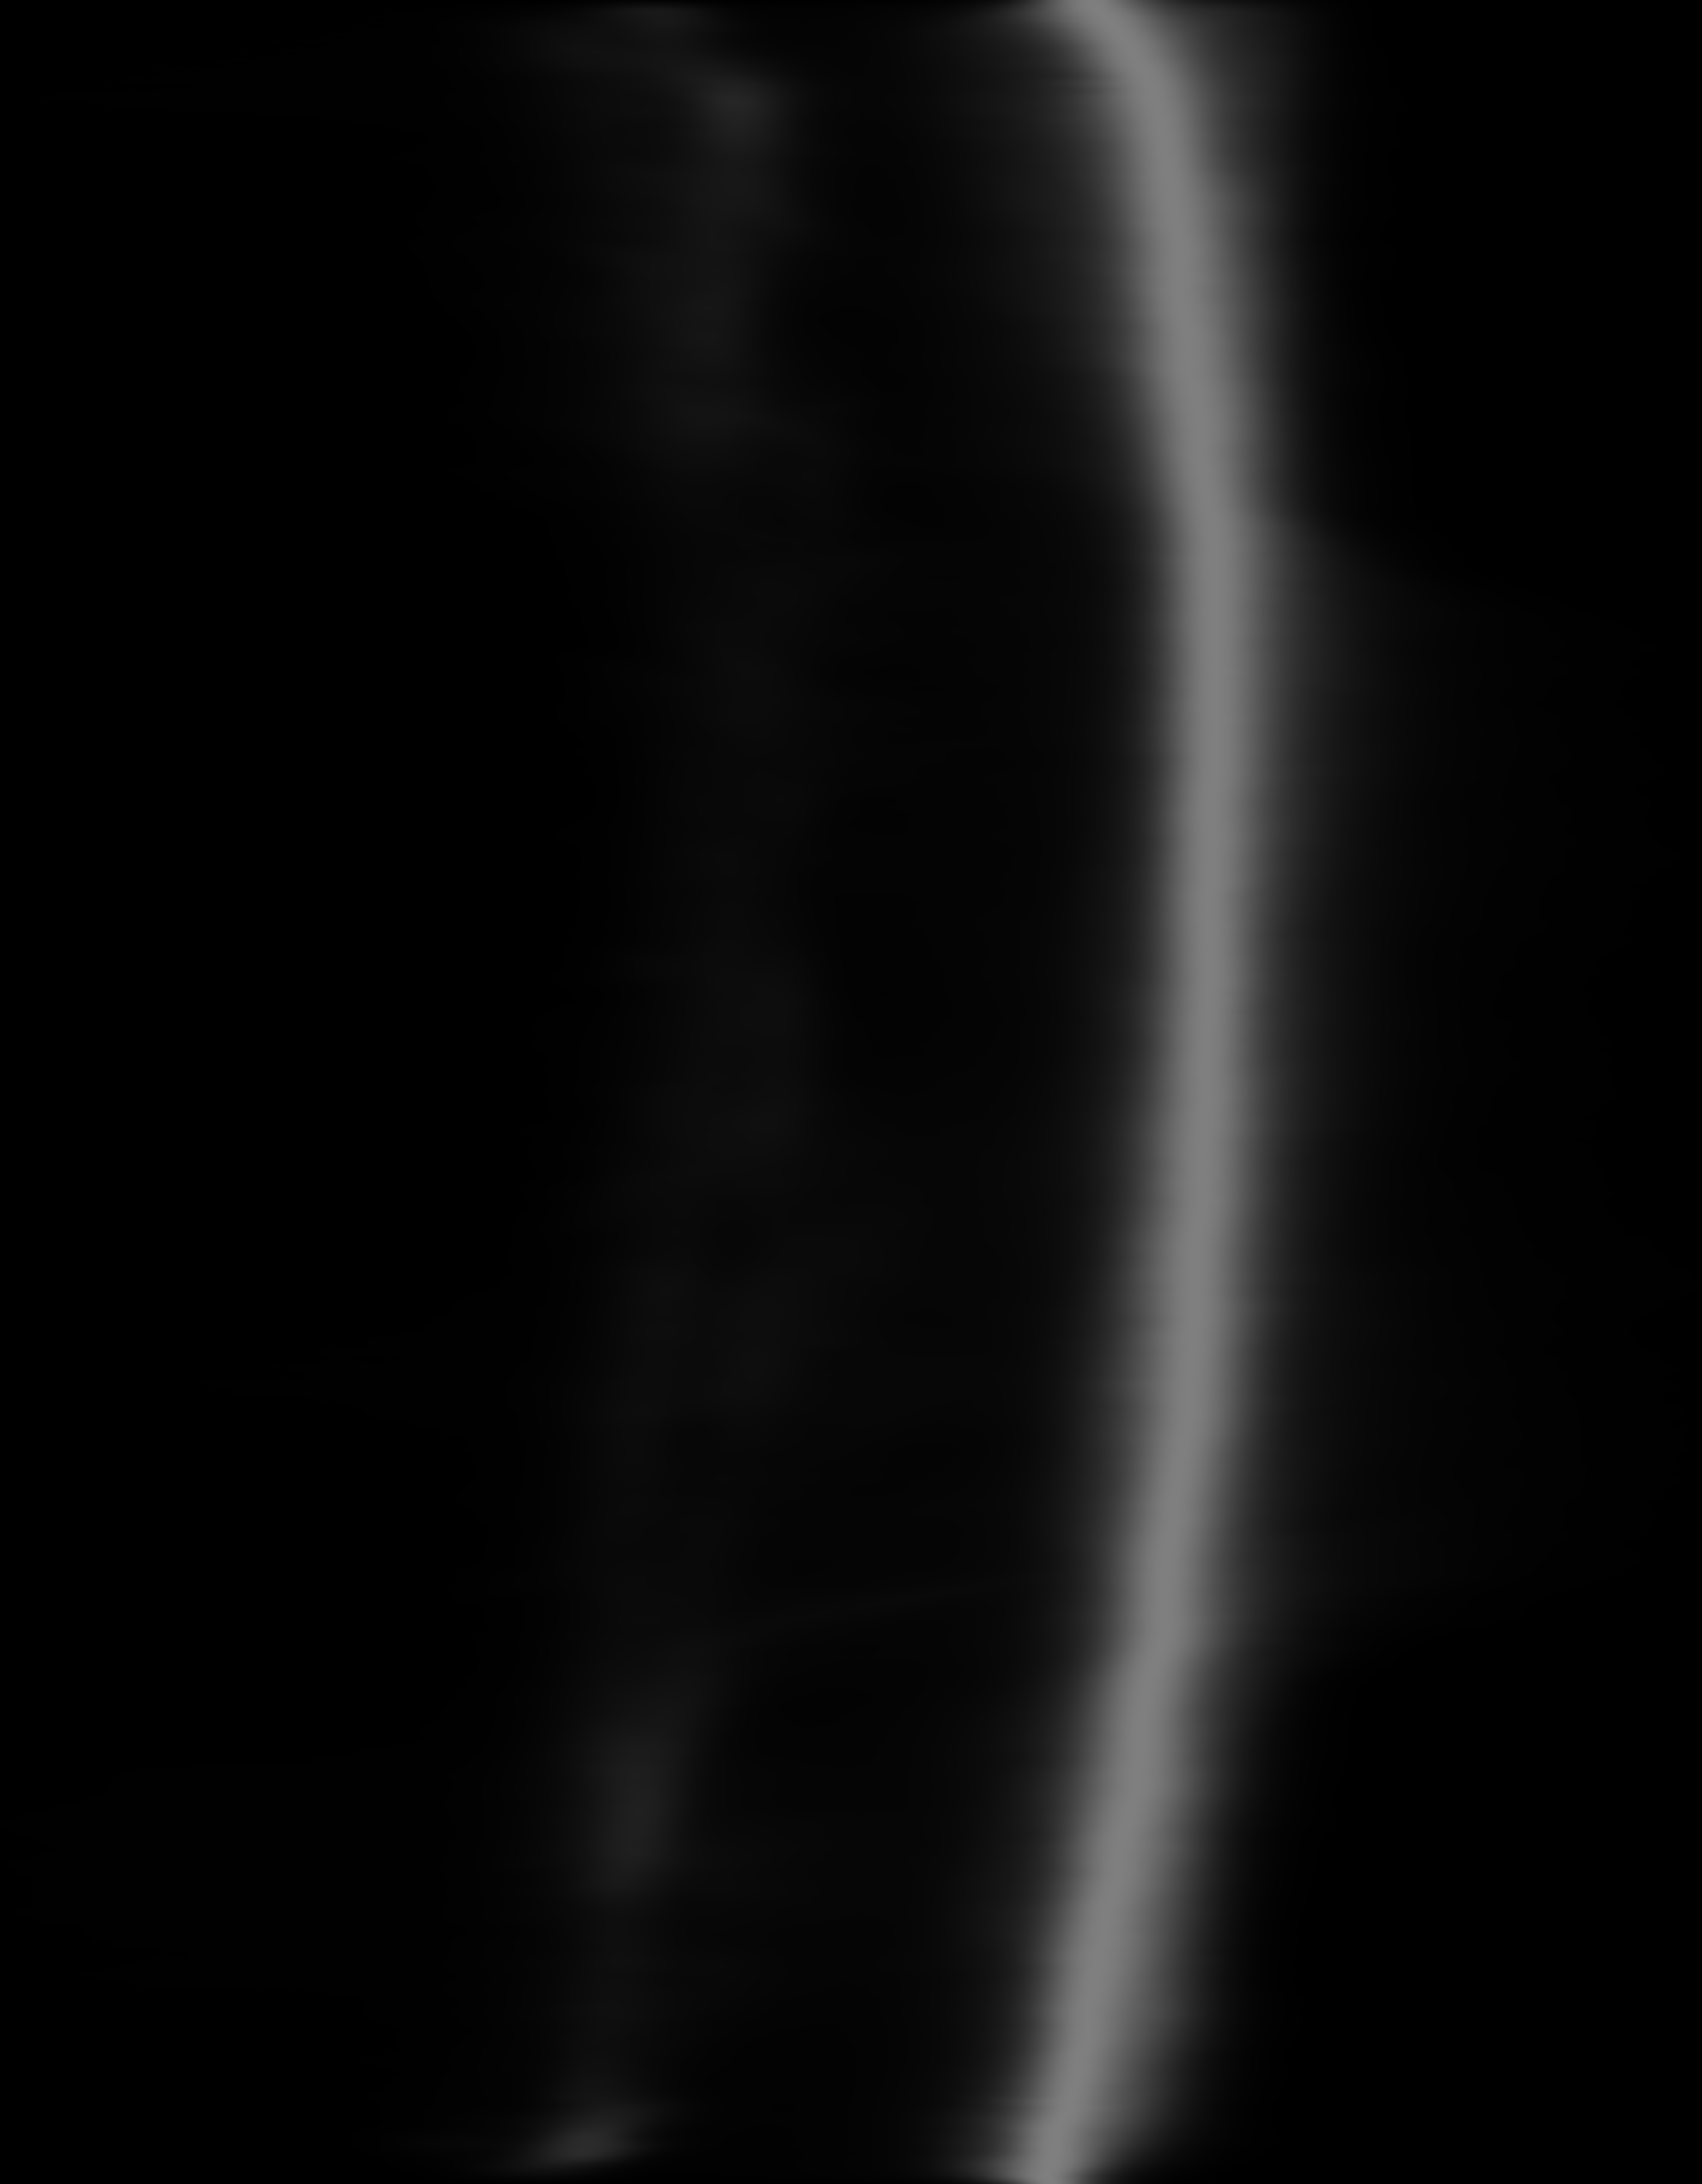
\includegraphics[width=.49\linewidth]{xb-bone_region3.png}
    %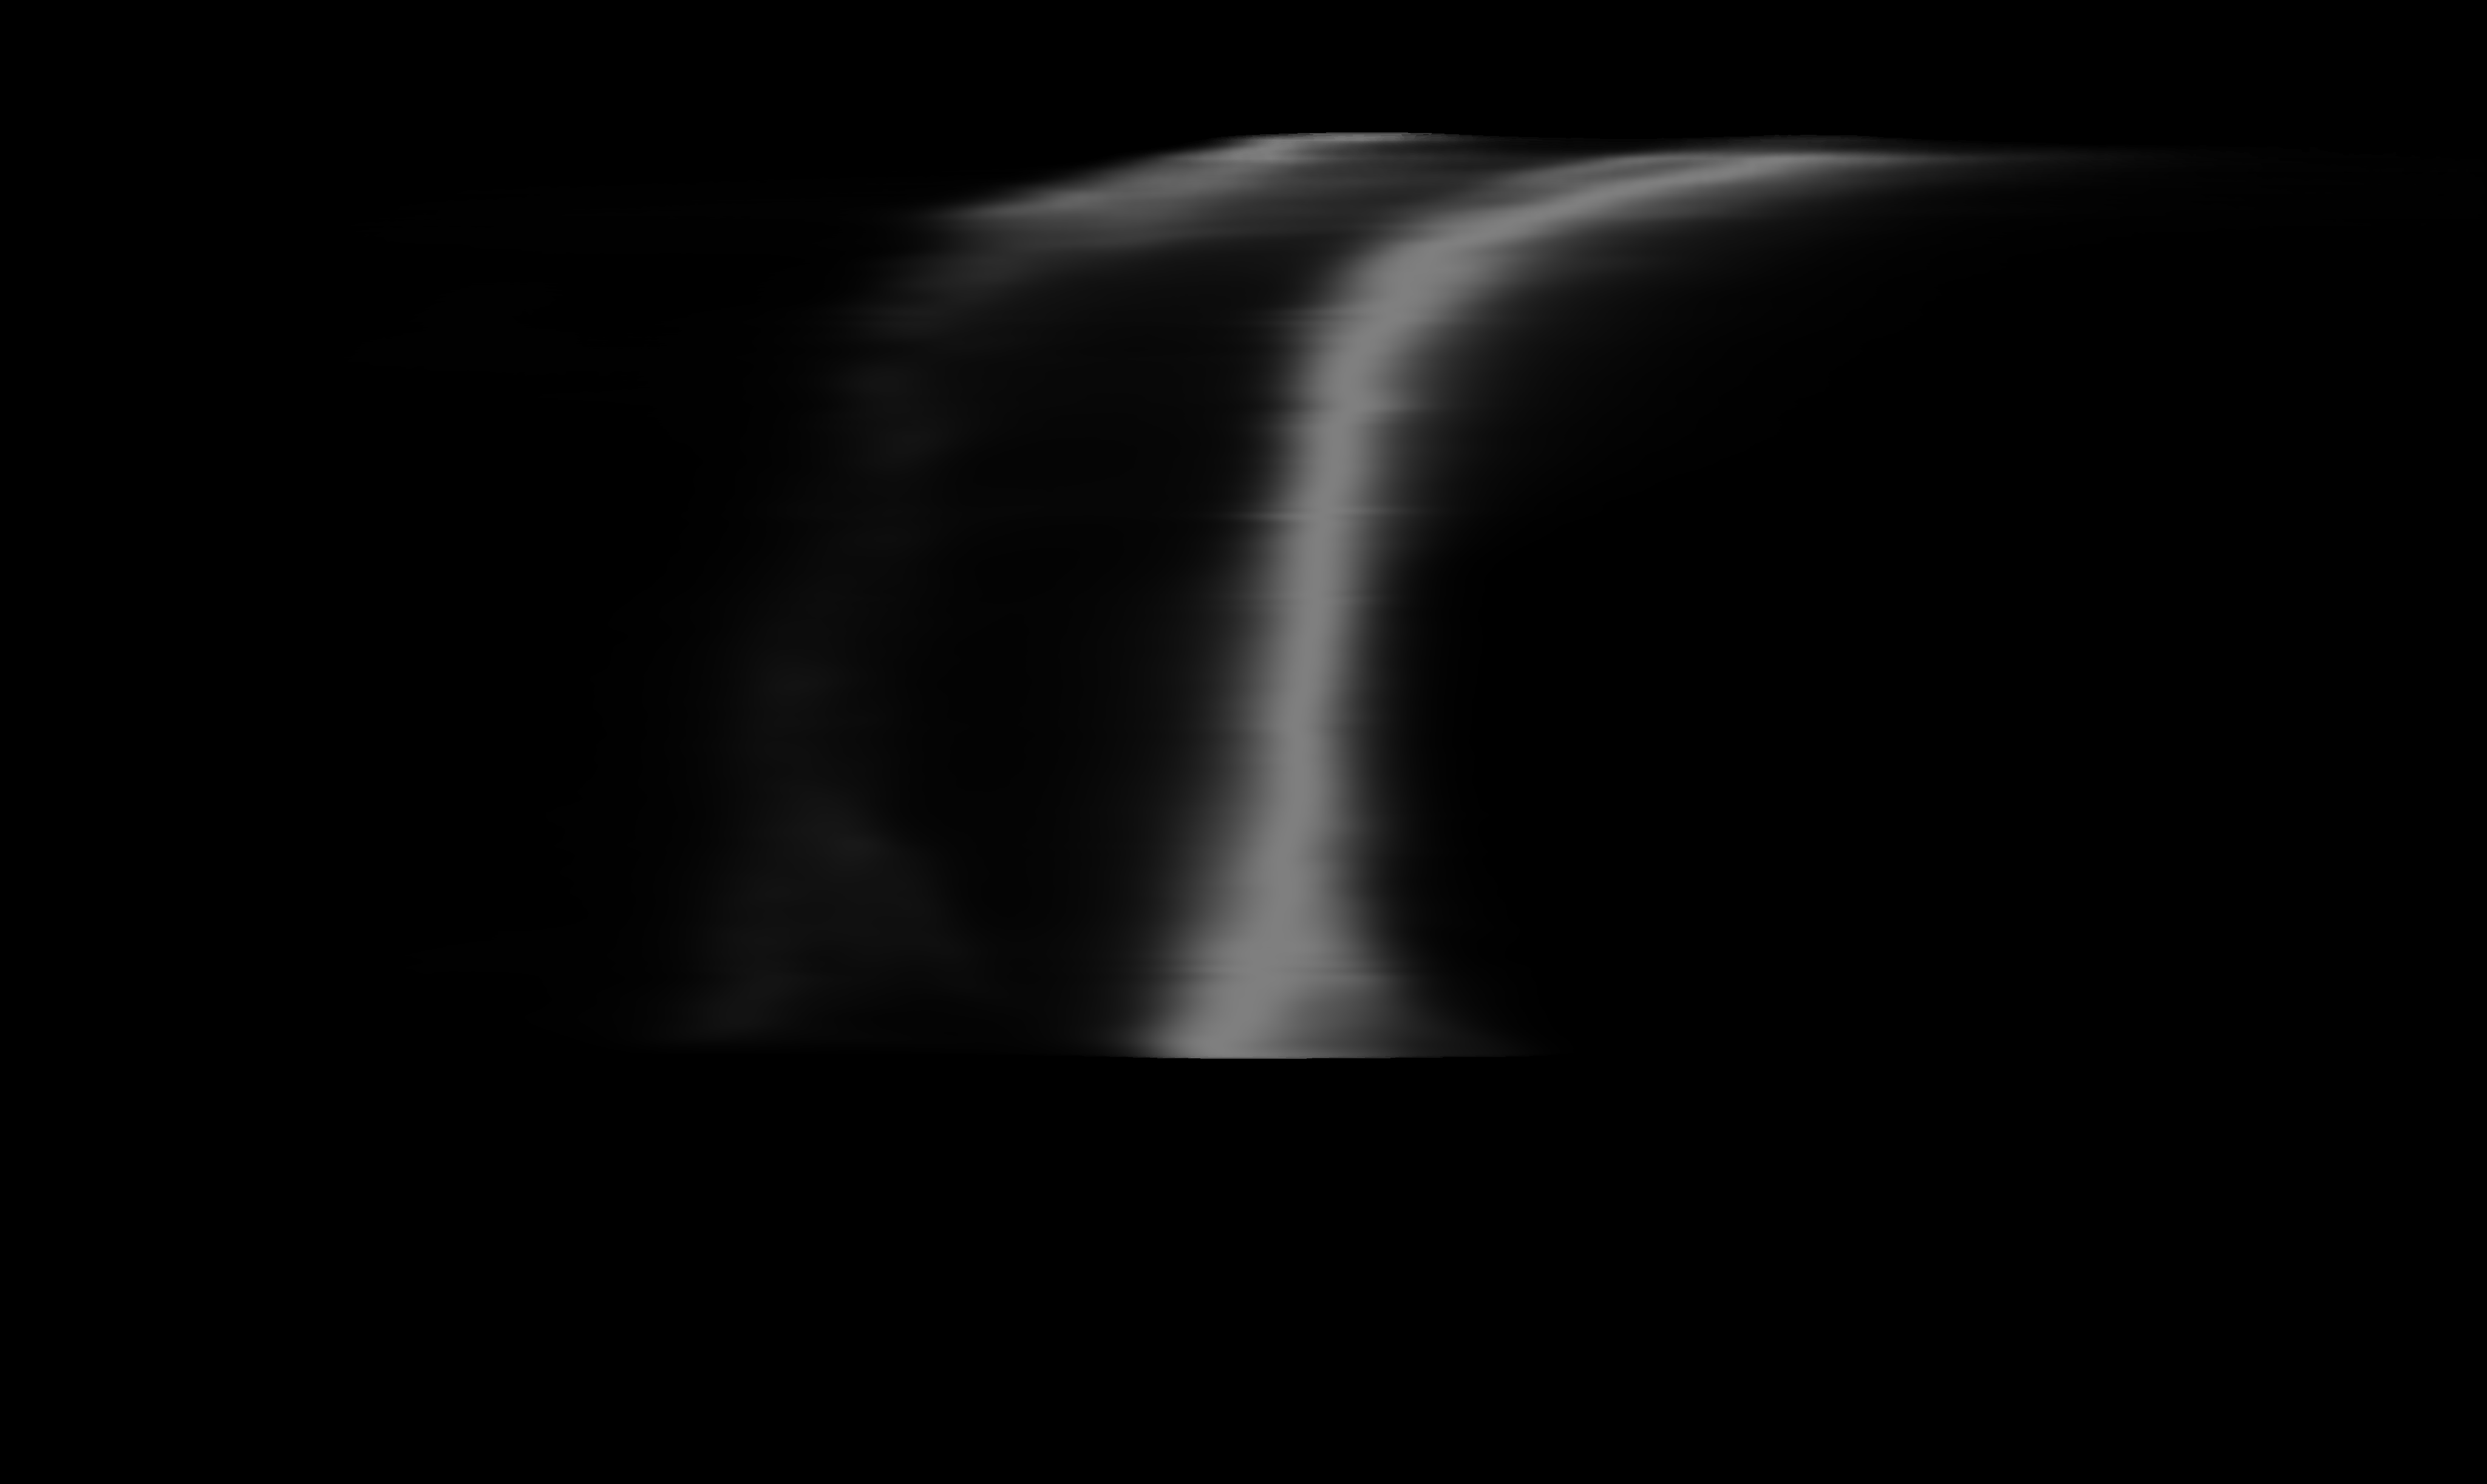
\includegraphics[width=\linewidth]{rb-bone_region3.png}
    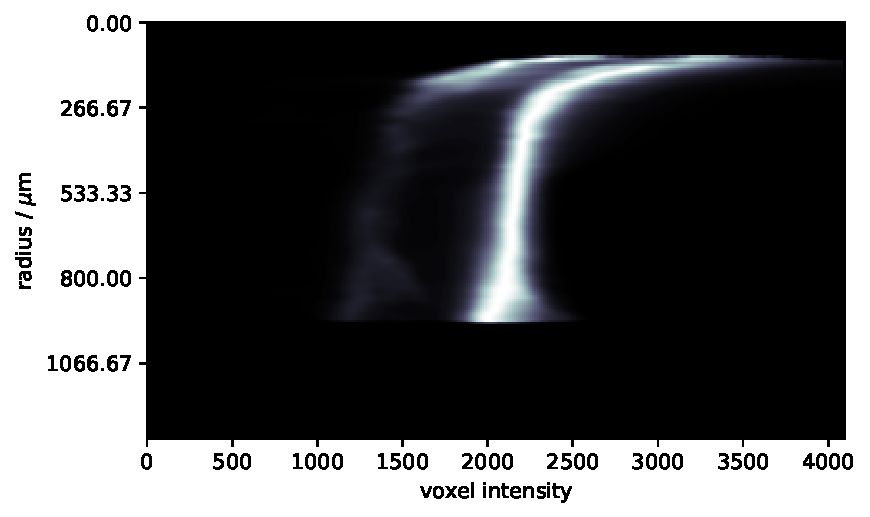
\includegraphics[width=\linewidth]{rb-bone_region3.pdf}
    \caption{2D radius histogram. The y-axis depicts radius, with the x-axis being voxel value.}
    \label{fig:2dhists}
\end{figure}

\subsection{Field histograms}
%Show that the fields can perfectly seperate
%discuss all the way to implant contact
In order to obtain spatial information based on the relation to the implant, we construct two
\textit{field} representations: Euclidian Distance Transform (EDT) and Diffusion.

%EDT is good overall, but difficult close to the implant.
EDT computes each voxel as the Euclidian distance to the implant.  This makes for a generally good
representation for all but the voxels that are close to the implant. The shortcoming near the implant
is mainly due to the fact that the voxels in the grooves of the implant have the same distance, and
thus the same value, as voxels next to the threads of the implant. This is shown in~\Cref{fig:edt-vs-diffusion}.
As discussed in~\Cref{sec:beam-hardening}, the implant produces a \textit{glowin}g effect, which
should be corrected by having higher field values for voxels surrounded by implant.

%Use diffusion to "zoom in" on the implant, as it is good close to the implant, but throws everything far away into the same bin
To get better correction close to the implant, we utilize diffusion where the implant "glows" further
accumulating the value when a voxel is surrounded by implant. This is shown in~\Cref{fig:edt-vs-diffusion},
where the voxels in the grooves are affected by multiple implant voxels. A slice of the resulting
diffusion field can be seen in~\Cref{fig:field-slice}.

\begin{figure}
    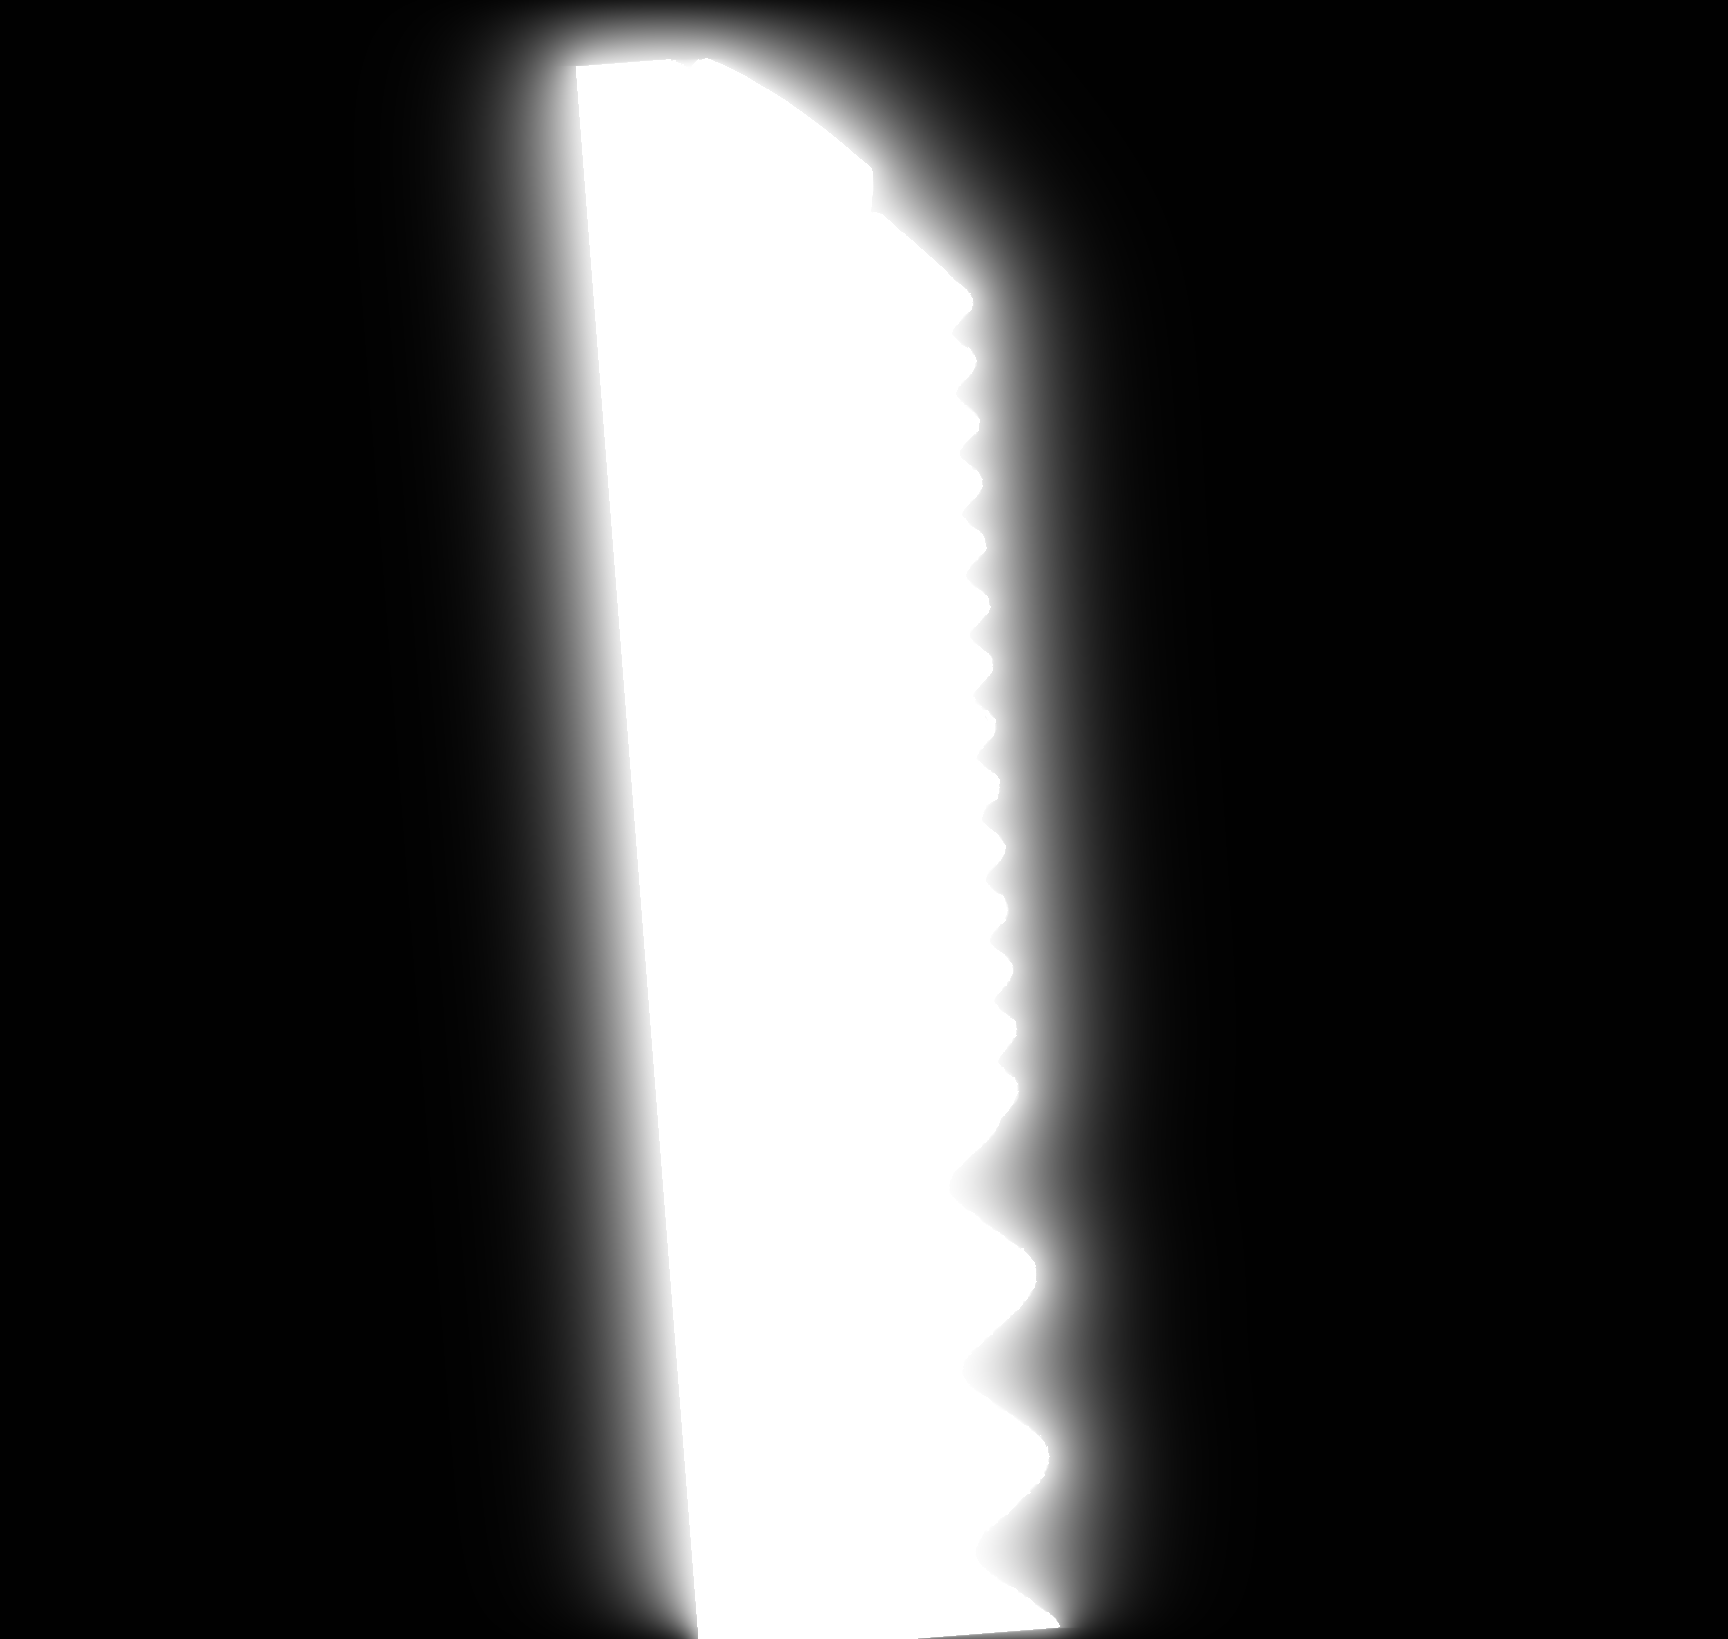
\includegraphics[width=\linewidth]{770c_pag-gauss-yz.png}
    \caption{A slice of the diffusion field in the YZ plane.}
    \label{fig:field-slice}
\end{figure}

\begin{figure}
    \vspace{-1.5cm}
    \centering
    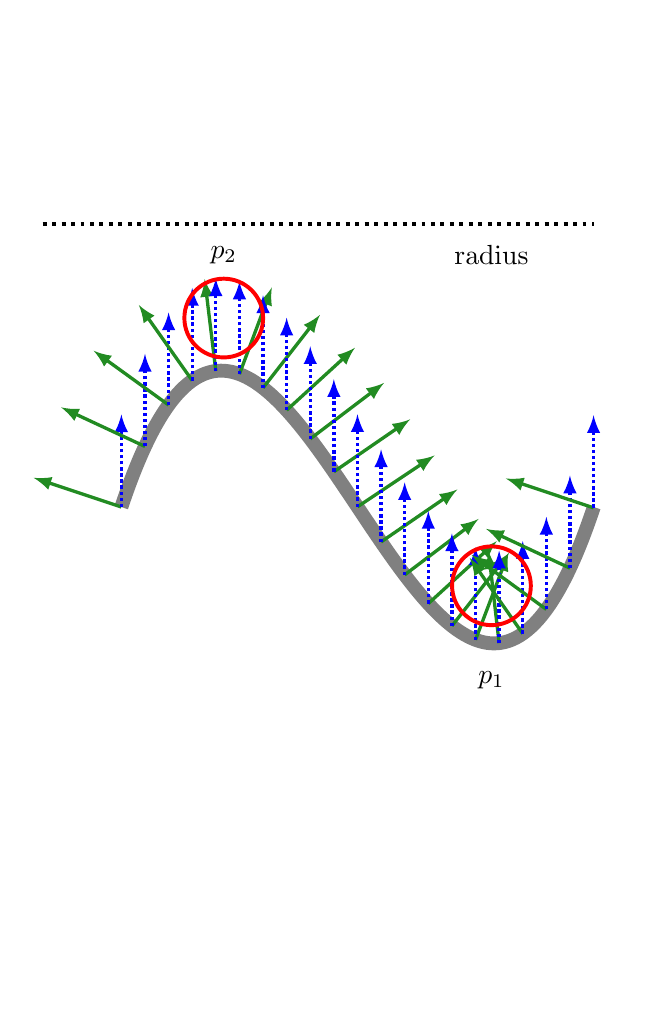
\begin{tikzpicture}[scale=2.0]
        \draw[gray,line width=5pt] (0,0)
        .. controls (1,3) and (2,-3) .. (3,0)
        \foreach \p in {0,5,...,100} {
          node[sloped,inner sep=0cm,above,pos=\p*0.01,
          anchor=south,
          minimum height=1.0cm,minimum width=1.0cm]
          (N \p){}
        }
        \foreach \p in {0,5,...,100} {
          node[midway,above,inner sep=0cm,above,pos=\p*0.01,
          anchor=south,
          minimum height=1.0cm,minimum width=1.0cm]
          (N2 \p){}
        }
        ;
        \foreach \p in {0,5,...,100} {
          \draw[-latex,ForestGreen, very thick] (N \p.south) -- (N \p.north);
          \draw[-latex,blue,densely dotted, very thick] (N2 \p.south) -- (N2 \p.north);
        }
        \draw[red, line width=0.5mm] (0.65,1.20) circle (0.25cm);
        \node at (0.65,1.60) {$p_2$};
        \draw[red, line width=0.5mm] (2.35,-0.5) circle (0.25cm);
        \node at (2.35,-1.10) {$p_1$};
        \draw[black, line width=0.5mm, dotted] (-0.5,1.8) -- (3.0,1.8);
        \node at (2.35,1.60) {radius};
      \end{tikzpicture}
      \vspace{-3.5cm}
    \caption{Visualization of the different field computations close to the implant threading in the YZ plane. The EDT is depicted in blue, where we see that $p_1$ and $p_2$ have the same distance. Diffusion is depicted in green, where we see multiple arrows contributing to the value of $p_1$. Using a radius of constant value, we see that the distance to the implant varies a lot.}
    \label{fig:edt-vs-diffusion}
\end{figure}

While diffusion works well on voxels close to the implant, it assigns the same value to the voxels
far from the implant. Therefore, an optimal solution is to use both the EDT and the diffusion field
to better represent both voxels that are far away, as well as the ones that are close to the implant.
We achieve this by adding the two fields together, producing a final combined field.

% Show that the distance to the implant in edt will be the same in the grooves of the screw compared
% to the threads of the screw. This is "fixed" with diffusion, as the grooves will be brigher as it
% is surrounded by more implant.

\subsection{Walkthrough of the method}
This section will describe each step of our method in detail. Going from tomography to a segmented tomography.

\subsubsection{Overview}
%Coarse steps, explain the idea
In order to reach the tissue-bone implant contact metric, we have the three coarse steps: compute the fields, segmentation using the fields, and extraction of the contact from the segmented tomography.

The steps of the field computation are:
\begin{itemize}
    \item Compute the EDT and Diffusion fields to give each voxel spatial information about its relation to the implant.
    \item Compute frequency distributions of voxel values as functions of field values as 2D histograms.
\end{itemize}

Then, in order to segment using the fields:
\begin{itemize}
    \item Find the materials within the 2D histograms as ridges, using image processing techniques.
    \item From the ridges, compute initial approximate frequency distributions of each material, which are then optimized to fit the 2D histograms.
    \item From the optimized distributions, we derive probability distributions for material classification. These distributions approximate the conditional probabilities $P(m|v,x)$ that a particular voxel belongs to material $m$ given that it has voxel value $v$ and field value $x$.
    \item Apply the probability distributions to the tomography, segmenting the voxels into the different materials.
\end{itemize}

Finally, to produce the tissue-bone implant contact metric:
\begin{itemize}
    \item From the segmented tomography, we compute the blood network of the bone regions to further extract which soft tissue voxels that are blood vessels.
    \item This blood network is used alongside the the segmented bone to produce the final metric.
\end{itemize}

%\james{TODO: Forklar bedre. Adskil ny segmenteringsmetode og anvendelse til BIC}

These steps are also summarized in the flow chart in~\Cref{fig:flowchart}.

\begin{figure}
    \centering
    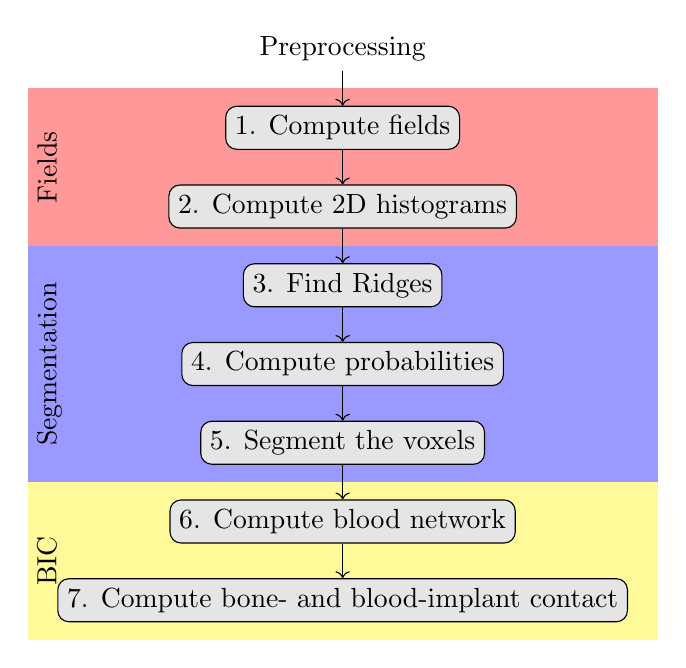
\begin{tikzpicture}
        \fill[red!40] (-4,.5) rectangle (4,-1.5);
        \fill[blue!40] (-4,-1.5) rectangle (4,-4.5);
        \fill[yellow!40] (-4,-4.5) rectangle (4,-6.5);
        \node[rotate=90, anchor=north] (field) at (-4,-.5) {Fields};
        \node[rotate=90, anchor=north] (segment) at (-4,-3) {Segmentation};
        \node[rotate=90, anchor=north] (bicc) at (-4,-5.5) {BIC};

        \node       (prep)  at (0, 1) {Preprocessing};
        \node[draw, fill=black!10, rounded corners] (field) at (0, 0) {1. Compute fields};
        \node[draw, fill=black!10, rounded corners] (hists) at (0,-1) {2. Compute 2D histograms};
        \node[draw, fill=black!10, rounded corners] (curvs) at (0,-2) {3. Find Ridges};
        \node[draw, fill=black!10, rounded corners] (probs) at (0,-3) {4. Compute probabilities};
        \node[draw, fill=black!10, rounded corners] (segm)  at (0,-4) {5. Segment the voxels};
        \node[draw, fill=black!10, rounded corners] (blood) at (0,-5) {6. Compute blood network};
        \node[draw, fill=black!10, rounded corners] (bic)   at (0,-6) {7. Compute bone- and blood-implant contact};

        \path[draw, ->] (prep)  -- (field);
        \path[draw, ->] (field) -- (hists);
        \path[draw, ->] (hists) -- (curvs);
        \path[draw, ->] (curvs) -- (probs);
        \path[draw, ->] (probs) -- (segm);
        \path[draw, ->] (segm)  -- (blood);
        \path[draw, ->] (blood) -- (bic);
    \end{tikzpicture}
    \caption{Flowchart depicting the steps of the method.}
    \label{fig:flowchart}
\end{figure}

\subsubsection{Segmentation}
The overall segmentation is computed in steps 1-5. For each step we will describe the process, showing
the algorithm where applicable, along with the the intermediate results.

\vspace{\baselineskip}
\noindent\textit{\textbf{Step 1: Field computations}}
Both fields are computed from the implant mask, as described in~\Cref{sec:preprocess}.
EDT is computed using the Python package \texttt{edt}~\cite{pypi-edt}. It takes the implant mask and
sets every non-set voxel to be the Euclidian distance of the nearest implant voxel.

For diffusion, rather than solving the diffusion equation, we approximate it using multiple convolutions
of a 3D-Gaussian kernel. Furthermore, instead of a single pass with a 3D-kernel, we apply 3 $\times$ 1D
convolutions, one in each dimension, to the tomography. This obtains the same result as a regular 3D-Gaussian
kernel. The algorithm can be seen in~\Cref{alg:diffusion}, and the XZ-plane in~\Cref{fig:field-slice}.

\begin{algorithm}
    \caption{Diffusion approximation.}
    \label{alg:diffusion}
    \begin{algorithmic}
        \Function {Diffusion} {$voxels[n_z*n_y*n_x]$, $repitions$, \newline \indent \indent $kernel[2*k+1]$}
            \State $S \gets [n_y * n_x, n_x, 1]$
            \State $N \gets [n_z, n_y, n_x]$
            \State $buf_0[:] \gets voxels[:]$
            \For {$rep$ \textbf{in} $repitions$}
                \For {$dim$ \textbf{in} $dimensions$}
                    \For {$z,y,x$ \textbf{in} $0{:}n_z,0{:}n_y,0{:}n_x$}
                        \State $X \gets [z,y,x]$
                        \State $i_{start} \gets - \min (k, X[dim])$
                        \State $i_{end} \gets \min (k, N[dim] - X[dim] - 1)$
                        \State $i_{global} \gets z*S[0] + y*S[1] + x*S[2]$
                        \For {$i$ \textbf{in} $i_{start}:i_{end}$}
                            \State $i_{offset} \gets i_{global} + i*S[dim]$
                            \State $buf_1[index] \gets buf_0[i_{offset}] * kernel[i+k]$
                        \EndFor
                    \EndFor
                    \State $buf_0[:] \gets buf_1[:]$
                \EndFor
            \EndFor
            \Return $buf_0$
        \EndFunction
    \end{algorithmic}
\end{algorithm}

%EDT + Diffusion
To obtain a good seperation both close to the implant and far away, we combine the two fields into a
single one as shown in~\Cref{eq:field-comb}.

%\begin{algorithm}
%    \caption{Field combination}
%    \label{alg:field-comb}
%    \begin{algorithmic}
%        \Function {field\_combine} {$f_{edt}, f_{dif}$}
%            \State $r \gets f_{dif} - \frac{f_{edt}}{\max (f_{edt})}$
%            \State $r \gets r - \min (f_{dif})$
%            \State $r \gets \frac{r}{\max (f_{dif})}$
%
%            \Return $r$
%        \EndFunction
%    \end{algorithmic}
%\end{algorithm}

\begin{equation}
    \label{eq:field-comb}
    \begin{split}
        f_{combined} &= \frac{f_{diffusion} - \frac{f_{edt}}{\max (f_{edt})} \min (f_{diffusion})}{\max (f_{diffusion})}
    \end{split}
\end{equation}

\vspace{\baselineskip}
\noindent\textbf{Step 2: 2D histograms} \\

From the combined fields we compute a 2D-histogram with the field value on the y-axis and the voxel
value on the x-axis.  This allows us to see the distribution of voxel values, based on their
relative position from the implant. The algorithm for the field-histogram can be seen in~\Cref{alg:field-hist}
along with a plot of the resulting histogram in~\Cref{fig:field-hist}. We see that the voxel values
shift based on their closeness to the implant, which clearly results in two seperable distributions.

\begin{algorithm}
    \caption{Field 2D histograms.}
    \label{alg:field-hist}
    \begin{algorithmic}
        \Function {Field\_hist} {$voxels[n_z,n_y,n_x]$, $field[n_z,n_y,n_x]$, $v_{bins}$, \indent \indent $v_{min}$, $v_{max}$, $f_{bins}$, $f_{min}$, $f_{max}$}
            \For {$z,y,x$ \textbf{in} $0{:}n_z,0{:}n_y,0{:}n_x$}
                \State $v \gets voxels[z,y,x]$
                \If {$v_{min} \leq v \leq v_{max}$}
                    \State $f \gets voxels[z,y,x]$
                    \If {$f_{min} \leq f \leq f_{max}$}
                        \State $v_i \gets (v_{bins} - 1) - \frac{v - v_{min}}{v_{max} - v_{min}}$
                        \State $f_i \gets (f_{bins} - 1) - \frac{f - f_{min}}{f_{max} - f_{min}}$
                        \State $h[f_i,v_i]{+}{+}$
                    \EndIf
                \EndIf
            \EndFor
            \Return $h$
        \EndFunction
    \end{algorithmic}
\end{algorithm}

\begin{figure}
    %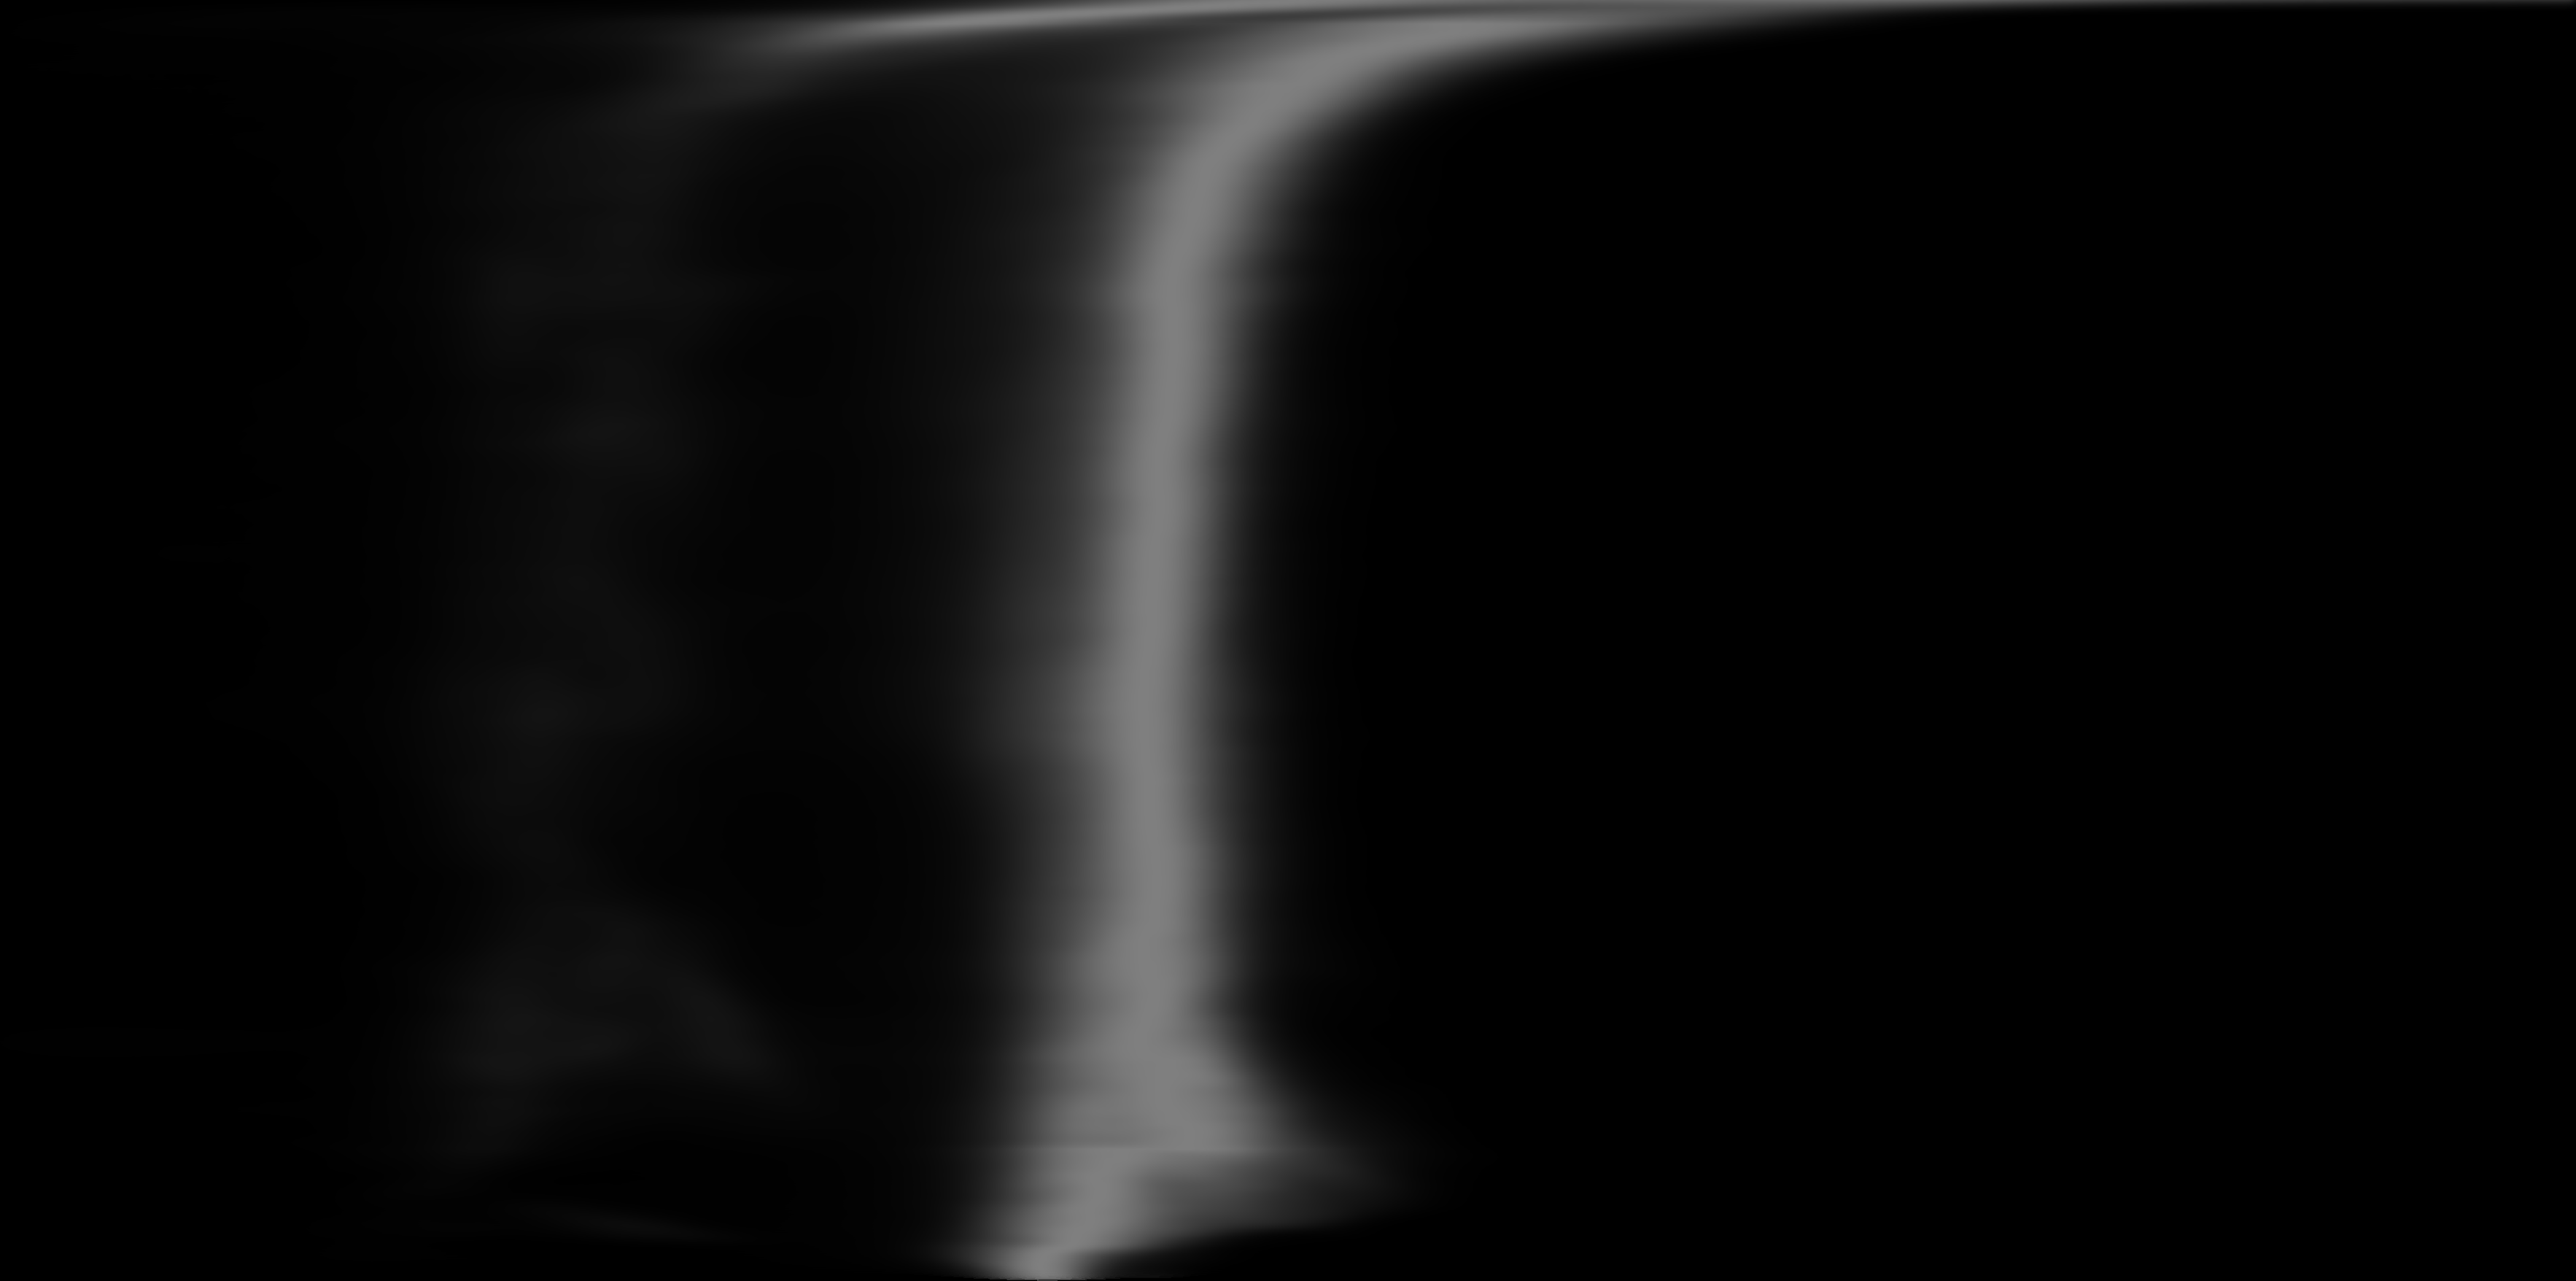
\includegraphics[width=\linewidth]{fb-edt-bone_region3.png}
    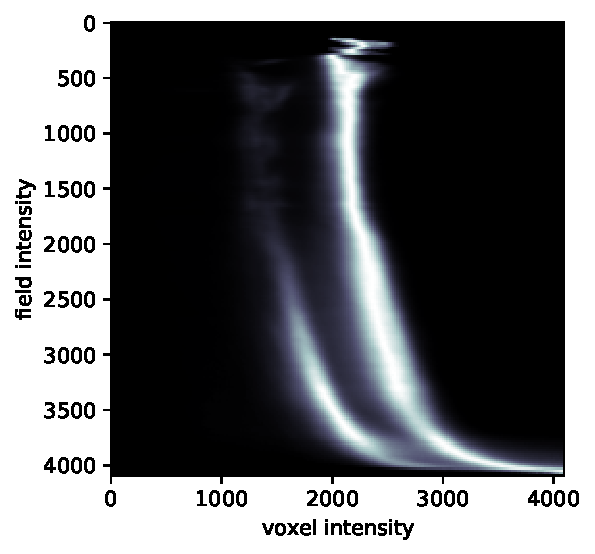
\includegraphics[width=\linewidth]{fb-gauss+edt-bone_region3.pdf}
    \caption{2D field histogram. Note that there are two clearly seperated ridges, which makes up
    different materials.}
    \label{fig:field-hist}
\end{figure}

\vspace{\baselineskip}
\noindent\textbf{Step 3: Isolate the materials} \\
The next step is to isolate the different materials spatially, which is done through the field-histogram.
For our first attempt, we applied Otsu's threshold to each each row in the 2D-histogram. While this
provided good results for two well defined distributions, it eventually began to fail. This was either
because of lack of samples, or because the histogram did not contain two distributions, which is an
underlying assumption of Otsu thresholding. These two effects occurred at the edges (both closest and
furthest from implant), which would bleed into the later steps of the segmentation process.

Rather than finding the threshold value in between the distributions, our next solution was to start
finding the distributions by finding the ridges of the 2D-histogram. We do this by applying a series
of image processing techniques, described in~\Cref{alg:material}. Each of the resulting contours
become their own material, which are then labeled as material 1 or 2 respectively for this particular
sample. For samples that would contain more than two distributions, the same algorithm should apply,
as long as the distributions does not overlap.

\begin{algorithm}
    \caption{Material isolation.}
    \label{alg:material}
    \begin{algorithmic}
        \Function {Materials} {$h[f_{bins}$, $v_{bins}]$, $\sigma$, $peak_{min}$, $k_x$, $k_y$, \newline \indent \indent $i_{dilate}$,$i_{erode}$, $t$}
            \For {$row$ \textbf{in} $0{:}f_{bins}$}
                \State $r \gets gaussian\_smooth(h[row,:], \sigma)$
                \State $p \gets find\_peaks(r, peak_{min})$
                \State $ps[p] \gets 1$
            \EndFor
            \State $kernel = cross\_kernel(k_x, k_y)$
            \State $d \gets dilate(ps, i_{dilate}, kernel)$
            \State $e \gets erode(d, i_{erode}, kernel)$
            \State $cs \gets find\_contours(e)$
            \For {$i$ \textbf{in} $0{:}|cs|$}
                \If {$size(cs[i]) > t$}
                    \State $l \gets draw\_contour(l, cs[i], i+1)$
                \EndIf
            \EndFor
            \Return $l$
        \EndFunction
    \end{algorithmic}
\end{algorithm}

\begin{figure*}
    % %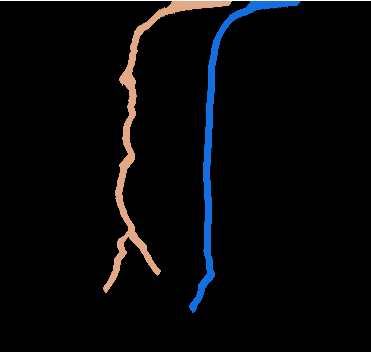
\includegraphics[width=0.5\linewidth]{curves_edt.png}%
    % %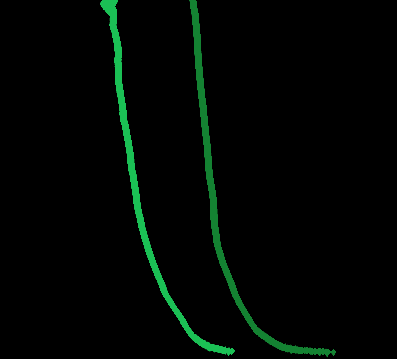
\includegraphics[width=0.5\linewidth]{curves_diffusion.png}
    % 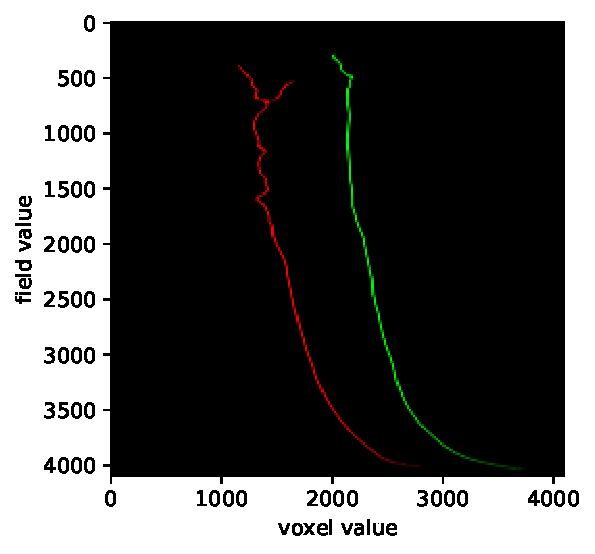
\includegraphics[width=\linewidth]{ridges_gauss+edt-bone_region3.pdf}
    % \james{will produce overall plot with probabilities}
    % \caption{Detected ridges from the combined field histogram.}
    % \label{fig:curves}
  \centering
  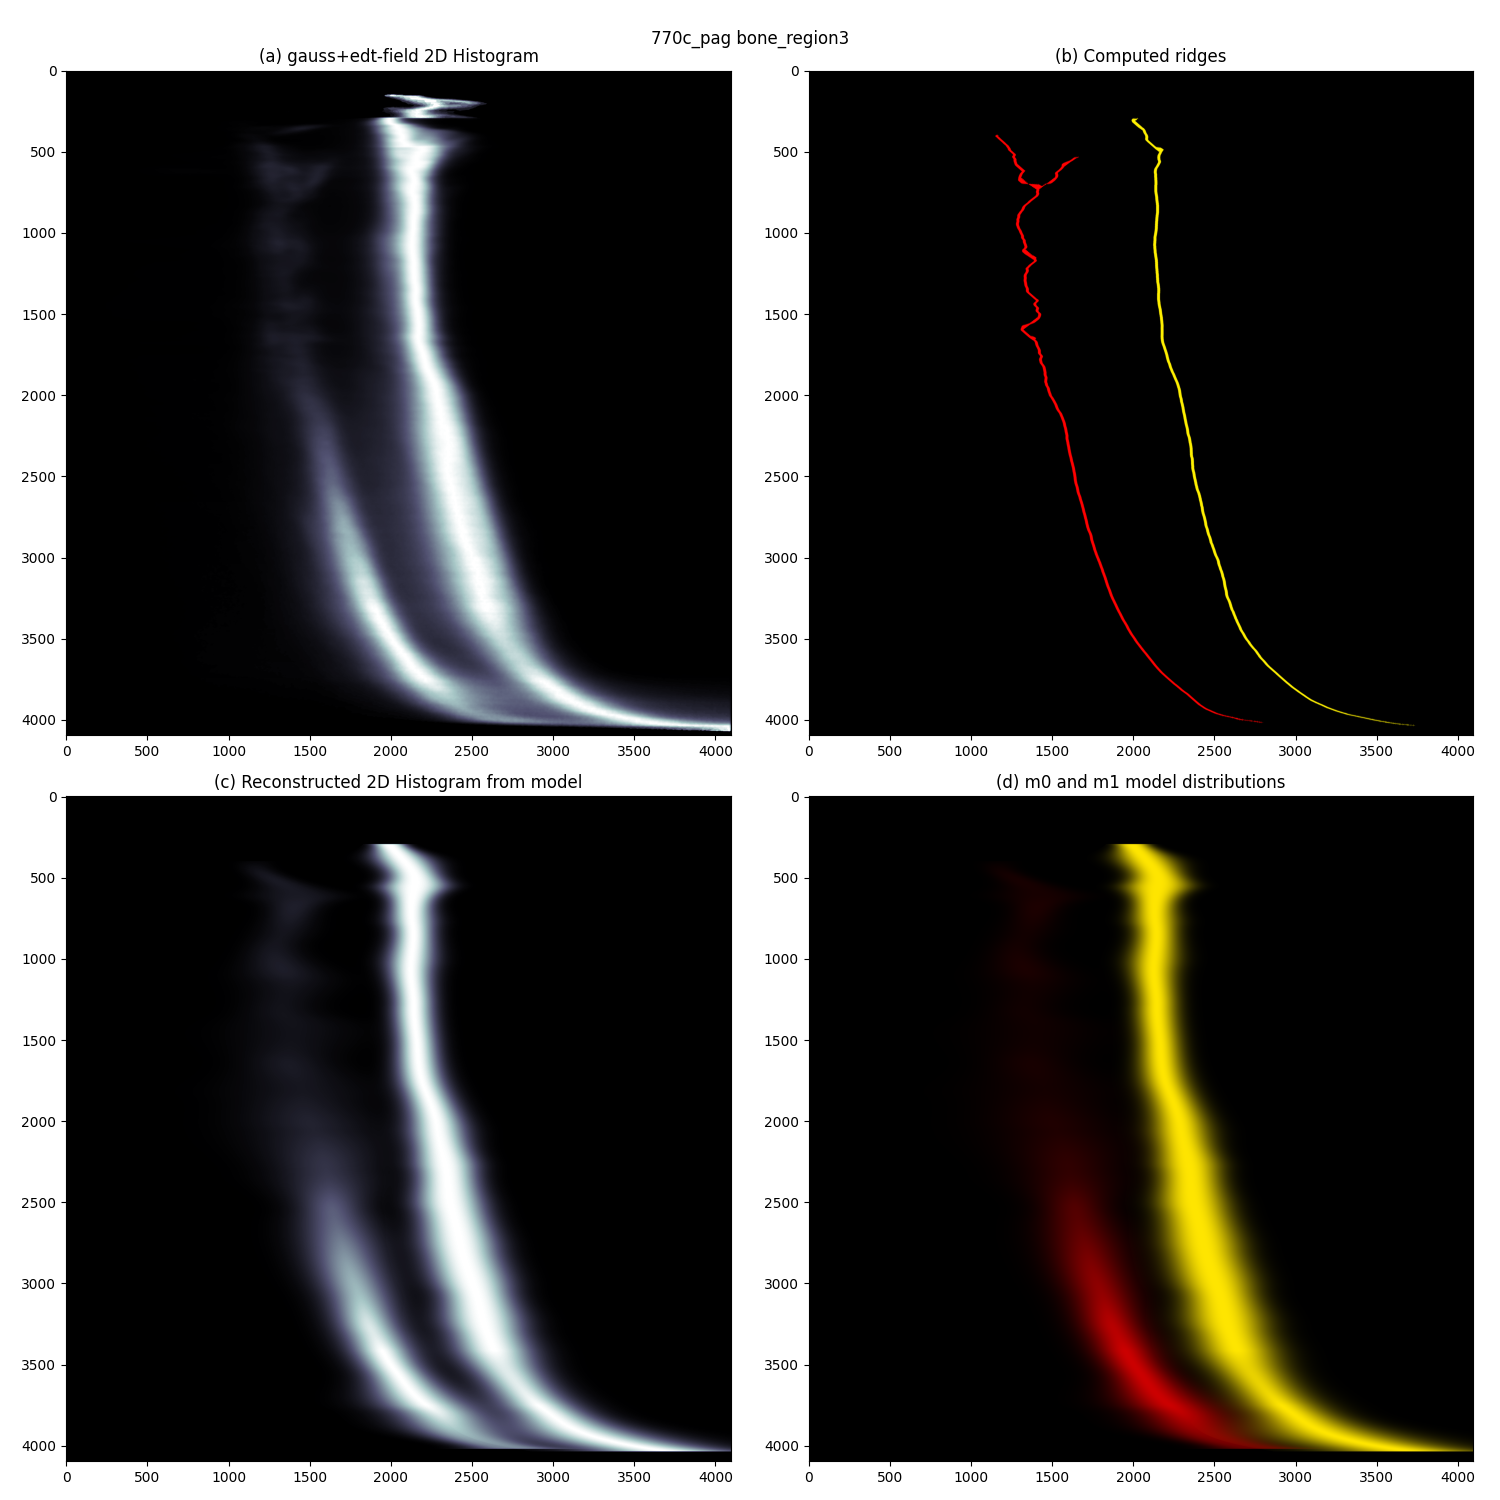
\includegraphics[width=.9\textwidth]{compute_probabilities_gauss+edt_bone_region3}\\
  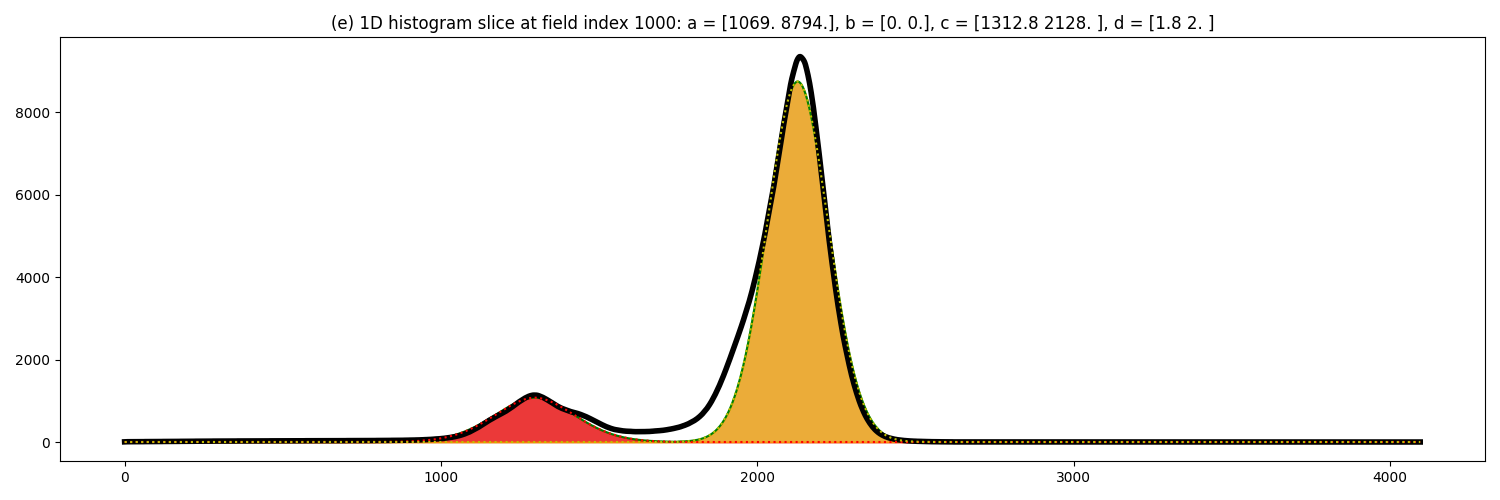
\includegraphics[width=.9\textwidth]{hist_slice_gauss+edt_bone_region3}\\
  \caption{(a) Measured 2D histogram for the compund diffusion+distance field from Step 2. (b)
    The detected ridges from Step 3. (c) Sum of computed frequency distribution models
    with optimized smooth piecewise cubic functions for parameters $a(\fval), b(\fval), c(\fval), d(\fval)$:
    this is the part of the 2D histogram explained by the smooth model. (d) The individual distributions evaluated
    on the 2D field-value$\times$ voxel-value grid. (e) A single 1D slice of the 2D histogram (black) together with
    the model frequency distributions. Red is soft-tissue, yellow is bone mineral.
  }
  \label{fig:curves-and-more}
\end{figure*}

\vspace{\baselineskip}
\noindent\textbf{Step 4: Compute models for material probability distributions} \\
Our goal is to obtain good conditional probability distributions $P(m|v,\xx)$
that model the likelihood of a voxel having material type $m$ as a function
both on its value $v$ and its position $\xx$ in space. For the probabilities
conditioned on the field values (distance or diffusion field), we model
the probability distributions $P(m|v,f(\xx))$ conditioned on
voxel- and field values. We want to make sure that these distribution
functions vary smoothly across space (or as a function of field values),
to ensure that we can identify the materials correctly across the entire
image: i.e., even though the frequency distributions look completely different
close to the titanium implant compared to the middle region or sample surface,
we can track the unbroken, smooth deformation to assign a global material
identity.

To this end, we first {\it model the frequency distributions} using the
2D histograms. Given that we are modeling materials $m=1,\ldots,M$,
we write the full 2D histogram as a sum of distributions
$g_m(\fval,v)$ modeling the described part, and an undescribed
residual $r(\xx,v)$.
\begin{equation}
  \label{eq:hist}
  H(\fval,v) = \sum_{m=1}^M g_m(\fval,v) + r(\fval,v)
\end{equation}
The residual is constrained to be non-negative, i.e., we must not explain
more voxels than the image contains.
The distribution functions can be chosen in any way that approximately
model the observed frequencies: we first used Gaussians with passable success,
but found that they dropped off too rapidly. We instead found excellent results
with the next-simplest model, leaving the exponential power free:
\begin{equation}
  \label{eq:dist-form}
  g_m(\fval,v) = a_m(\fval) e^{-b_m(\fval) |v-c_m(\fval)|^d_m(\fval)}
\end{equation}
where for each field value $\fval$
$a(\fval)$ is the distribution height at the center $v=c(\fval)$,
$b(\fval)$ is the exponential falloff rate, and $d(\fval)$ is
the exponential power ($d=2$ yields a Gaussian, $d=1$ a simple exponential).
In practice we found $1.5\le d \le 2$ to best match the actual frequency
distribution decay rates.

Using the ridges found in the previous step, we generate good starting
guesses and constraints for the distribution parameters
$a,b,c,d$:
For each field-value $\fval$ (corresponding to a row in the 2D histogram),
we initialize the starting approximation as:
\begin{equation}
  \label{eq:starting-guesses}
  \begin{split}
    c_m(\fval) &= \mathop{\mathtt{argmax}}_{v \text{ with }\lab[\fval,v] = m} H(\fval,v)    \\
    a_m(\fval) &= H(\fval,c_m(\fval))\\
    b_m(\fval) &= 3/\mathrm{width}_m(\fval)^2 \\
    d_m(\fval) &= 2
  \end{split}
\end{equation}
where we use half the distance to the center of ridge $m+1$ as the width
$\mathrm{width_m}(\fval)$, using the relation that $b = 3/w^d$ yields
a $5\%$ cutoff at $w$ when $1\le d \le 2$. This approximation
already yields a good approximation. Thus, the subsequent
optimization using the constrained quasi-Newton optimization method L-BFGS-B\cite{BFGS}
converges rapidly to an excellent fit. Each 1D histogram row is first optimized
independently in parallel: The resulting numerical functions
$a_m(\fval),\ldots,d_m(\fval)$ are then converted into piecewise cubic
functions using a least squares-based algorithm that ensures continuity
and differentiability across the piecewise segments. This lets us interpolate across
outliers due to noise, but equally important:
extrapolate our models smoothly into the regions very close to the implant, where
we don't have enough voxels to produce good statistics.

We finally obtain the {\it conditional probabilities} from the material frequency distribution
models $g_m$ as:
\begin{equation}
  \label{eq:Pm}
  P(m|v,f(\xx)) = \frac{g_m(v,f(\xx))}{H(v,f(\xx))}
\end{equation}
(well-defined where $H(v,\fval) > 0$, zero outside this region as $0\le g_m \le H$).



%%% Local Variables:
%%% mode: latex
%%% TeX-master: "main"
%%% End:


\vspace{\baselineskip}
\noindent\textbf{Step 5: Perform segmentation}

The final step of the segmentation process is to utilize the probabilities for segmentation.
This process is fairly straightforward, as each voxel is looked up in the probability distribution,
which carries the same shape as the field-histogram.

\begin{algorithm}
    \caption{Final segmentation from the probability distributions.}
    \label{alg:segment}
    \begin{algorithmic}
        \Function {Segment} {$voxels[n_z,n_y,n_x], p[f_{bins},v_{bins}],$ \newline \indent \indent $v_{bins}, v_{min}, v_{max}, f_{bins}, f_{min}, f_{max}$}
            \For {$z,y,x$ \textbf{in} $0{:}n_z,0{:}n_y,0{:}n_x$}
                \State $v \gets voxels[z,y,x]$
                \If {$v_{min} \leq v \leq v_{max}$}
                    \State $f \gets voxels[z,y,x]$
                    \If {$f_{min} \leq f \leq f_{max}$}
                        \State $v_i \gets (v_{bins} - 1) - \frac{v - v_{min}}{v_{max} - v_{min}}$
                        \State $f_i \gets (f_{bins} - 1) - \frac{f - f_{min}}{f_{max} - f_{min}}$
                        \State $result[z,y,x] \gets p[f_i, v_i]$
                    \EndIf
                \EndIf
            \EndFor
            \Return $result$
        \EndFunction
    \end{algorithmic}
\end{algorithm}

\subsection{Results of the field-segmentation}

Here we present the final output from the steps described above.

\begin{figure}
    \centering
    \begin{subfigure}[b]{\linewidth}
        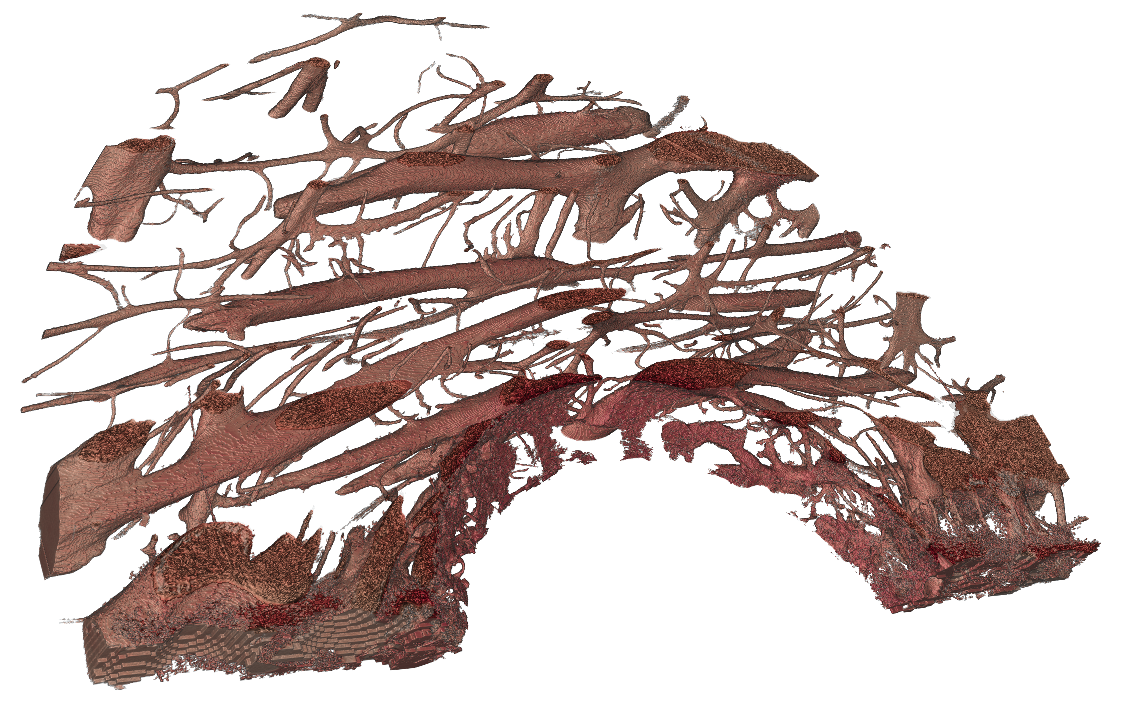
\includegraphics[width=\linewidth]{figures/blood_old_bone_100.png}
        % TODO opdater hvis en anden slice størrelse bliver brugt. voxel size = 3.75
        \caption{3D render of a $375\mu m \times 4230\mu m \times 6480\mu m$ slice of the blood network in the old bone region.}
        \label{fig:blood-old-slice}
    \end{subfigure}
    \begin{subfigure}[b]{\linewidth}
        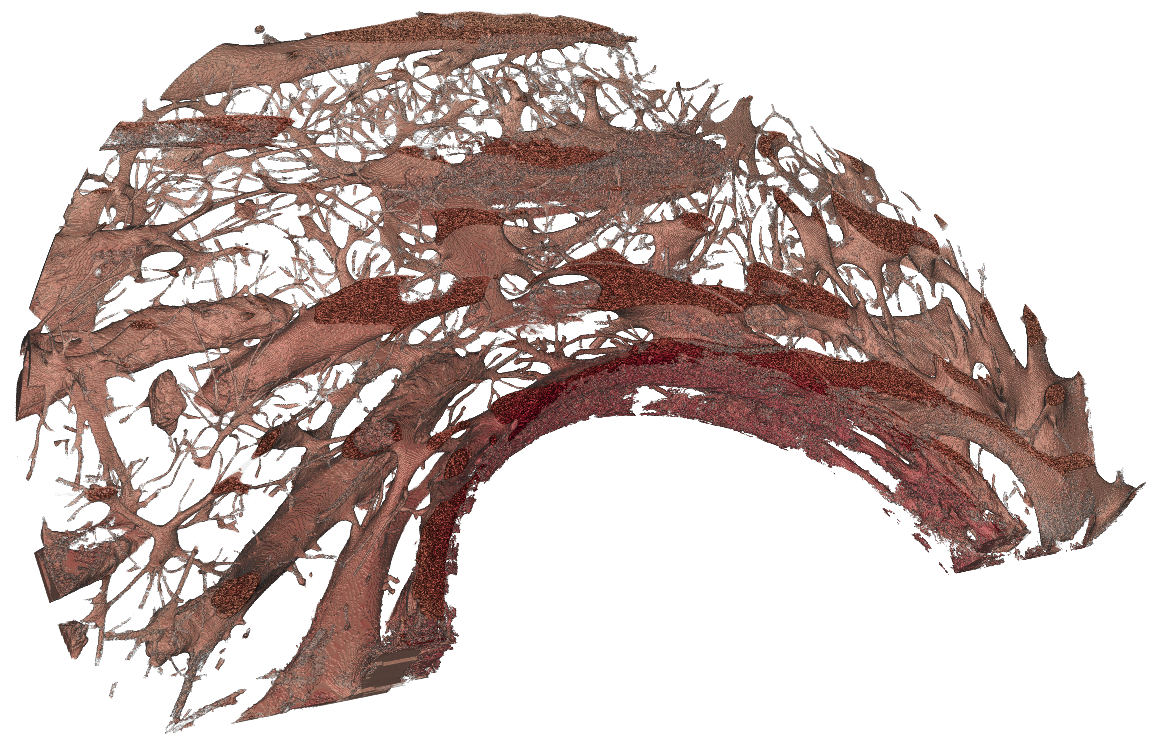
\includegraphics[width=\linewidth]{figures/blood_new_bone_100.png}
        \caption{3D render of a $375\mu m \times 4230\mu m \times 6480\mu m$ slice of the blood network in the new bone region.}
        \label{fig:blood-new-slice}
    \end{subfigure}
    \begin{subfigure}[b]{.45\linewidth}
        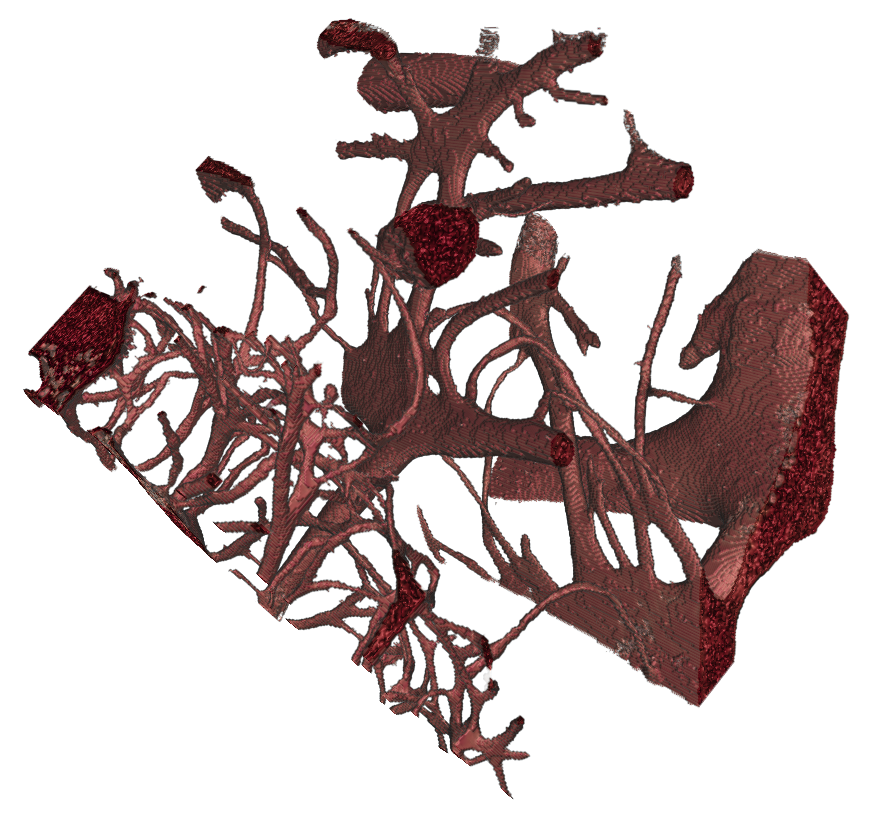
\includegraphics[width=\linewidth,height=\linewidth]{figures/blood_old_cube.png}
        \caption{3D render of a $1mm \times 1 mm \times 1 mm$ cube of the blood network in the old bone region.}
        \label{fig:blood-old-cube}
    \end{subfigure}
    \hfill
    \begin{subfigure}[b]{.45\linewidth}
        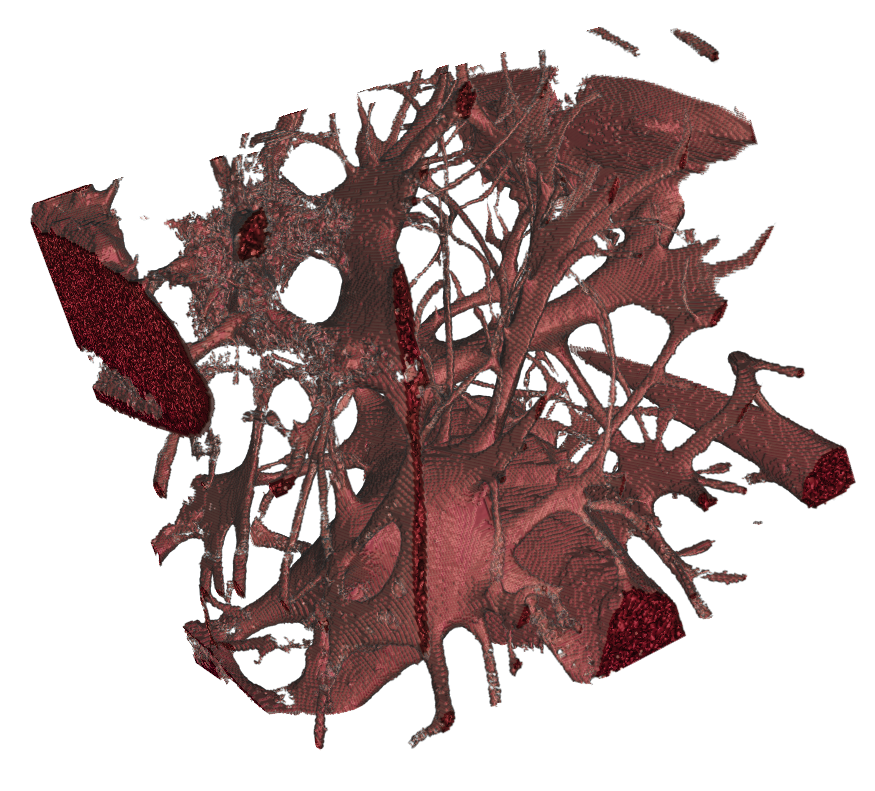
\includegraphics[width=\linewidth,height=\linewidth]{figures/blood_new_cube.png}
        \caption{3D render of a $1mm \times 1 mm \times 1 mm$ cube of the blood network in the new bone region.}
        \label{fig:blood-new-cube}
    \end{subfigure}
    \caption{3D renders of the blood network. All of the samples are generated from a 2x downsample of the full resolution. Note the difference between the the capillary network in the old bone region (\ref{fig:blood-old-slice},\ref{fig:blood-old-cube}) compared to the newly grown bone region (\ref{fig:blood-new-slice},\ref{fig:blood-new-cube}).}
    \label{fig:blood-network}
\end{figure}

\subsubsection{Sub-classification of soft tissue}

With a good separation of soft tissue and bone, we  map out the blood vessel network using connected
components analysis. The osteocytes are selected by volume and shape: For every connected component
in the feasible volume range, its principal axis and best ellipsoid is computed and checked against
the potential osteocyte shape.

\subsection{Visualizing bone-implant contact and blood-implant contact}

Once segmenter, tissue in contact with the implant can be studied using the
Euclidean Distance Transform (EDT) from the implant, restricted to the bone region. We can
simply mask the voxels that are within a thin shell of distances, $d_{min} < d(x,y,z) \le d_{max}$,
for example $d_{min} = 1\mu m$ to $d_{max} = 10\mu m$. We then sum over the masked voxels of each
tissue type to obtain and divide by the total to obtain the tissue-to-implant contact per area,
or study the distribution across the surface area qualitatively.

\subsubsection{Histology-comparison}

\begin{figure}
  \centering
  \begin{tabular}{c}
    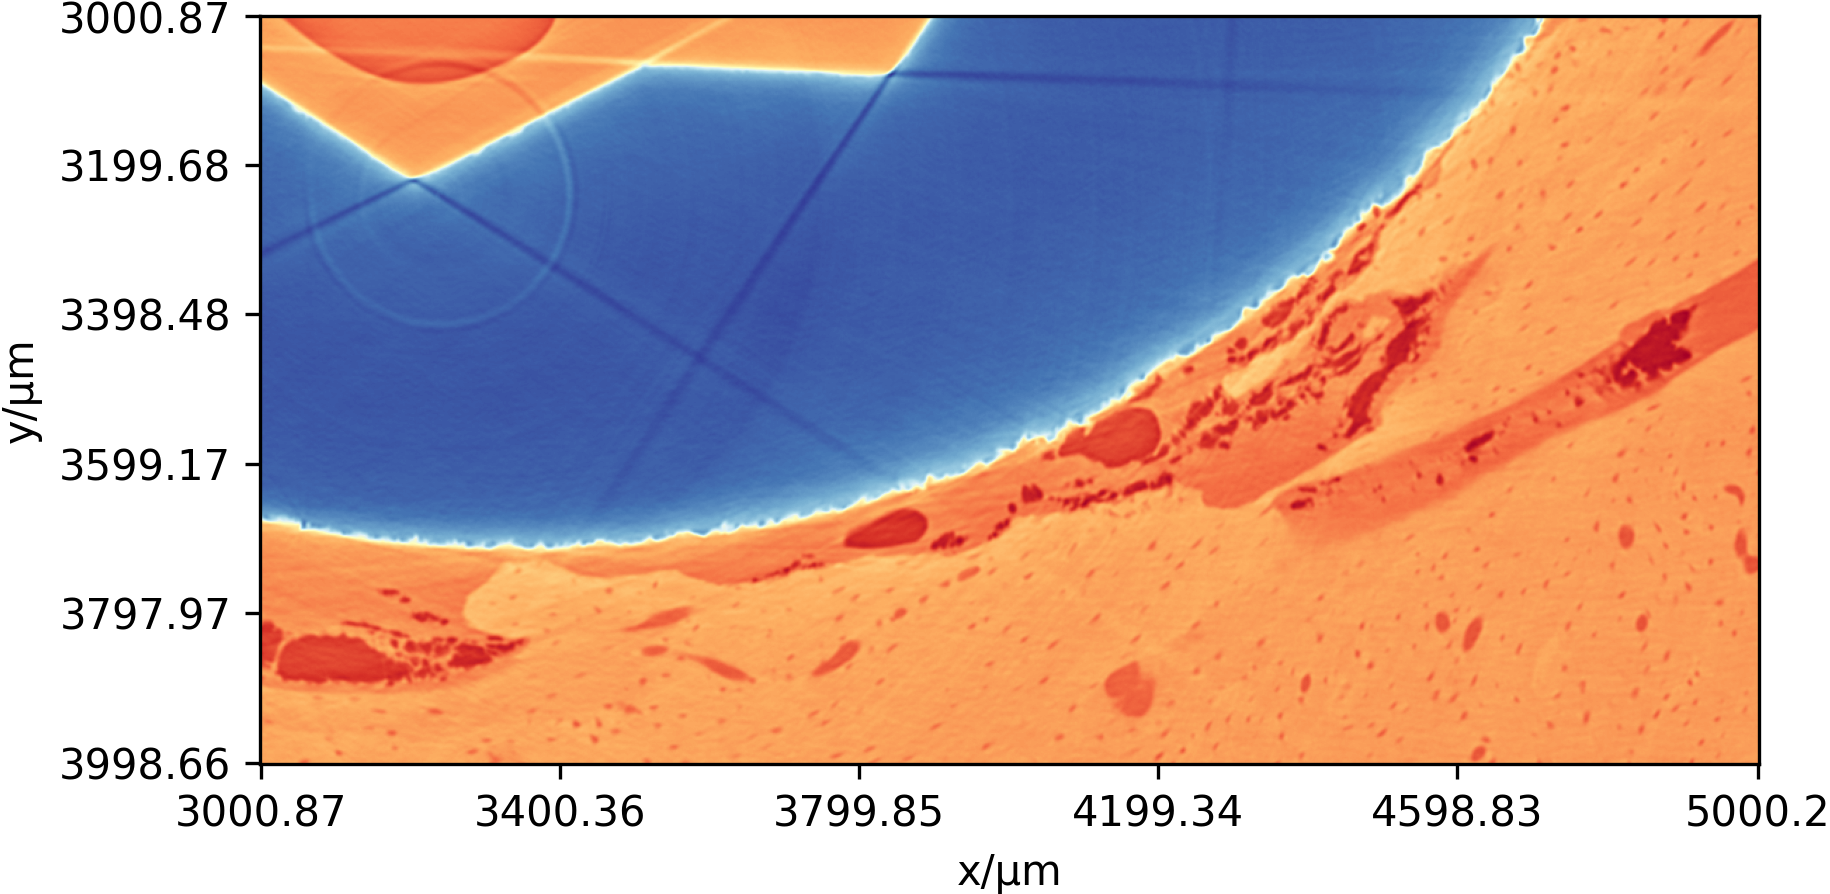
\includegraphics[width=\linewidth]{770c_pag-bic-xy-1x} \\
    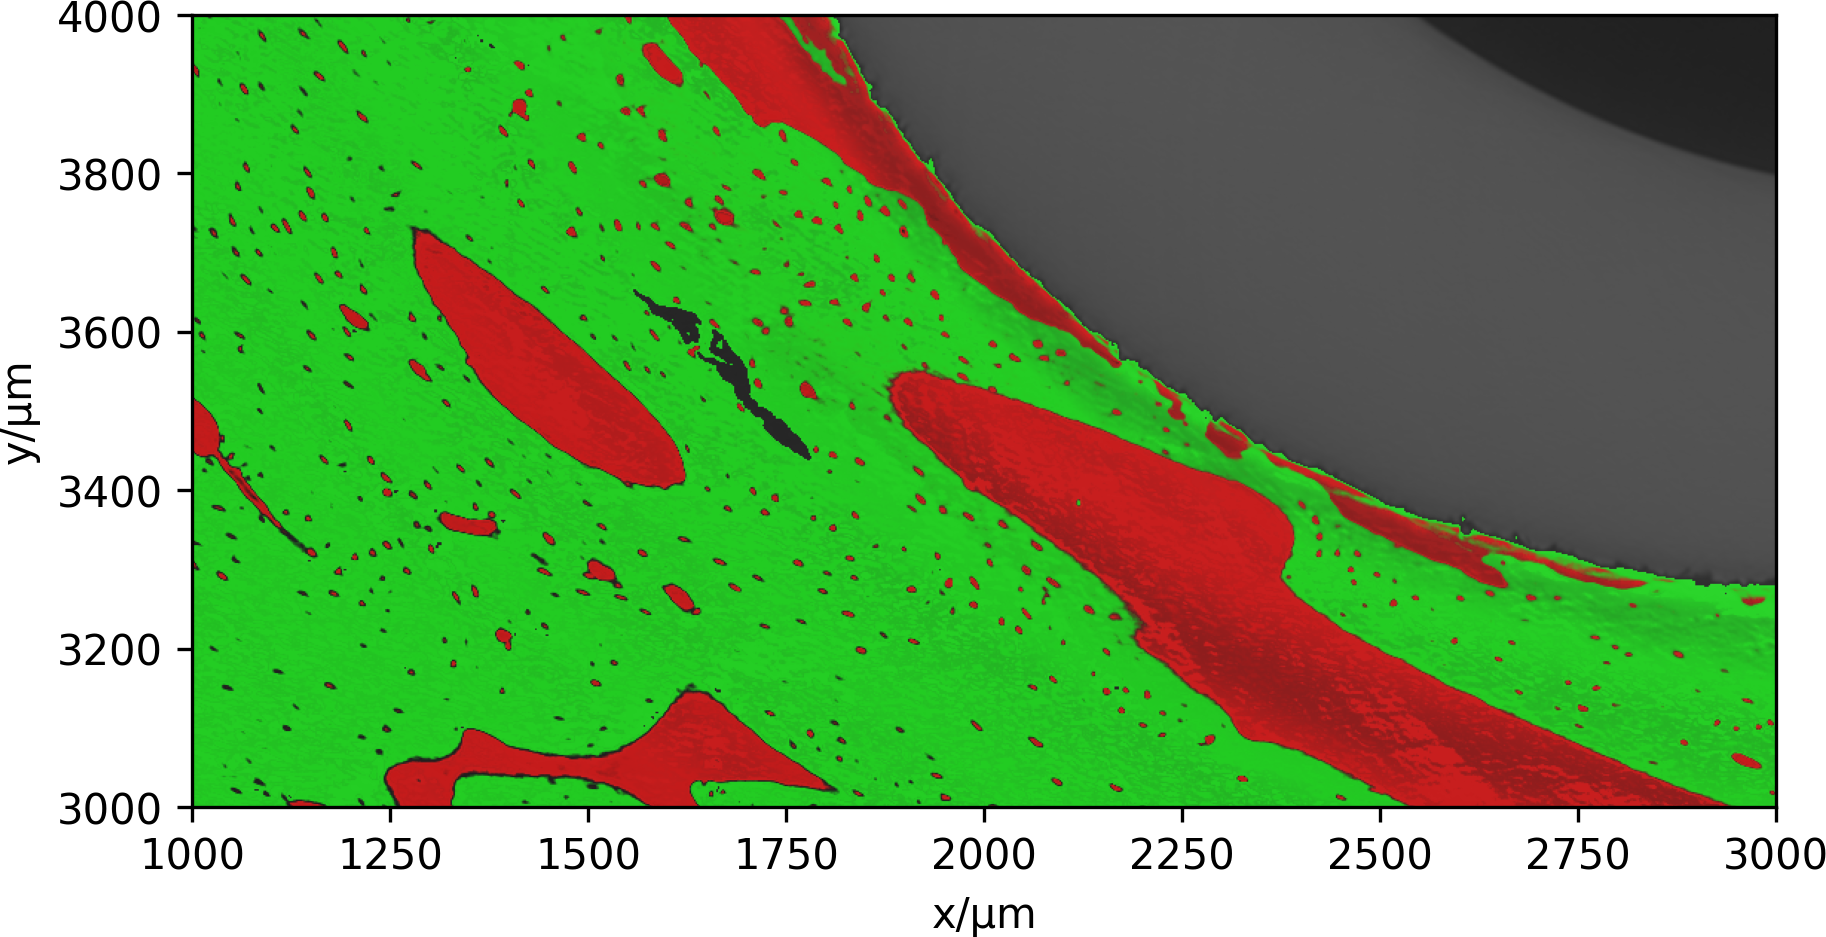
\includegraphics[width=\linewidth]{770c_pag-bic-P01-xy-1x}
  \end{tabular}
  \caption{TBW}
  \label{fig:histology-comparison1}
\end{figure}

\begin{figure}
  \centering
  \begin{tabular}{c}
    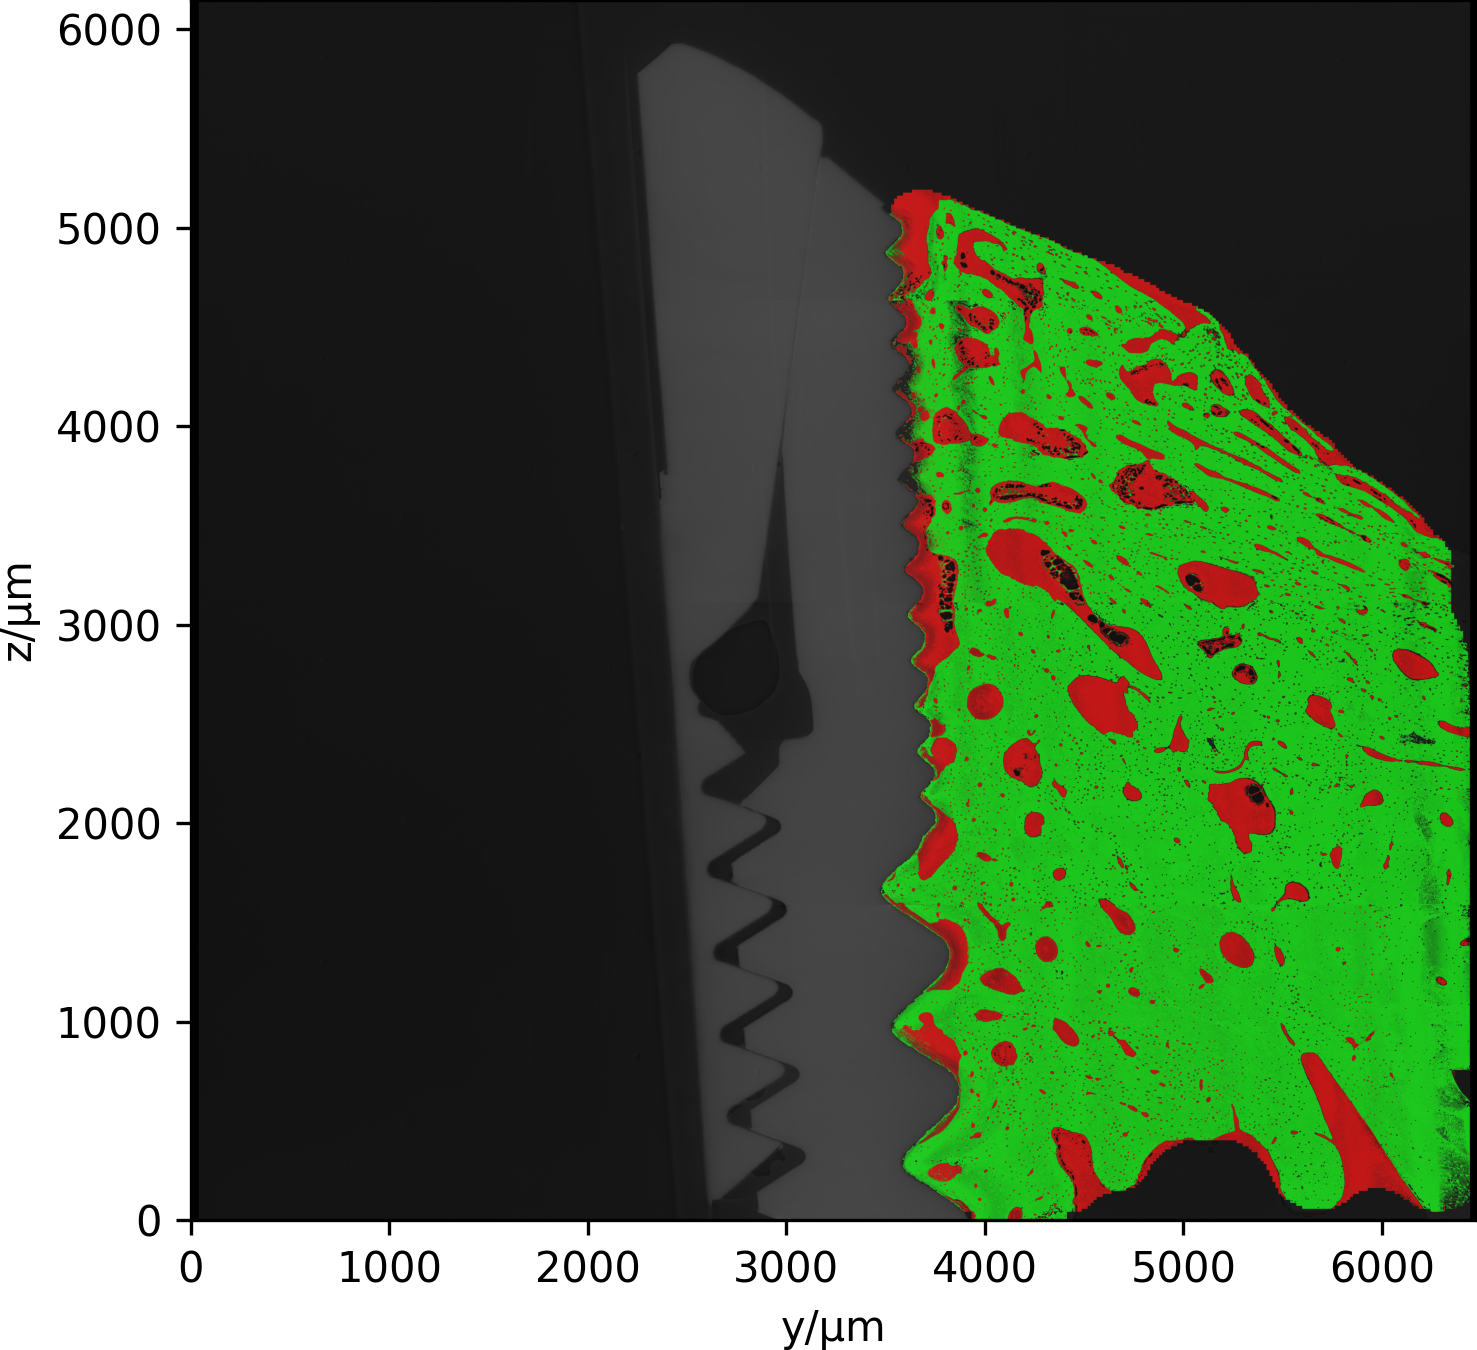
\includegraphics[width=\linewidth]{770c_pag-full-P01-yz-1x} \\
    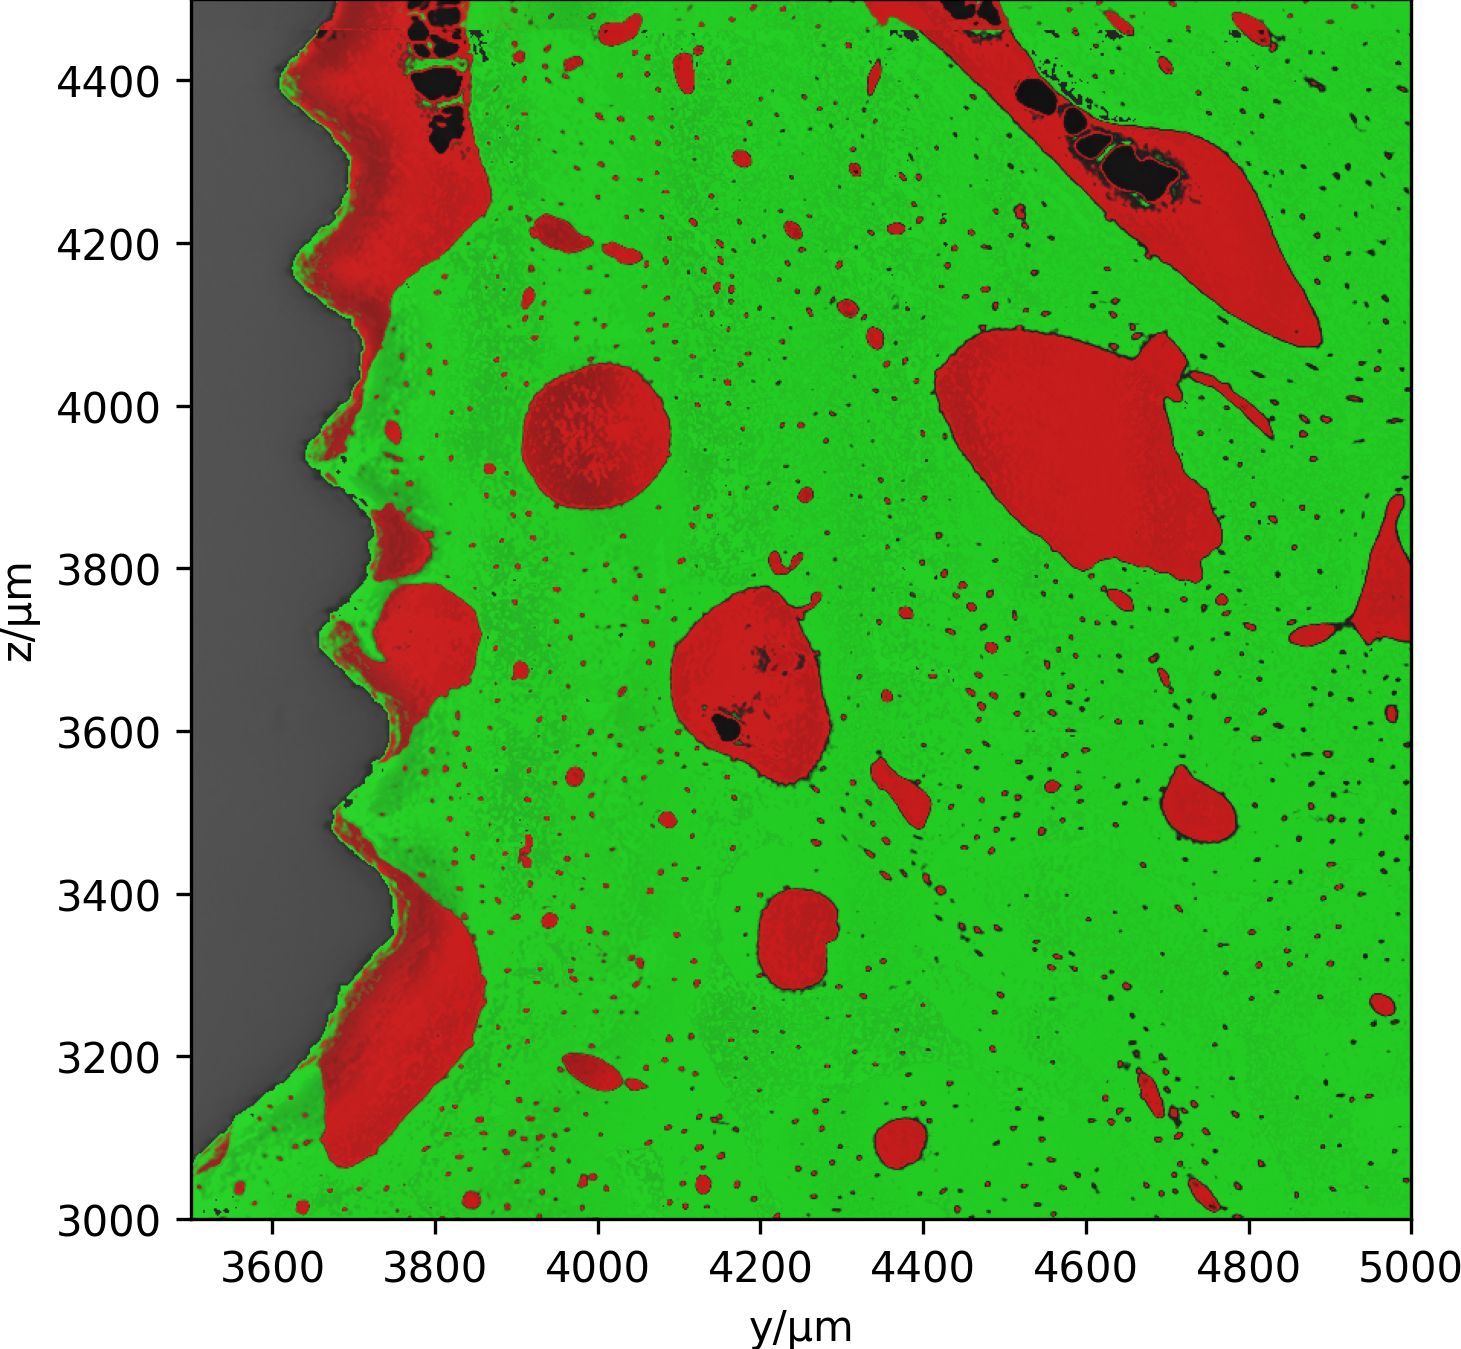
\includegraphics[width=\linewidth]{770c_pag-bic-P01-yz-1x}
  \end{tabular}
  \caption{TBW}
  \label{fig:histology-comparison2}
\end{figure}

% \subsubsection{Cylindrical projection of implant contact-surface}

% In this subsection, we show how to map the tissue-to-implant contact surface for visual inspection.
% The challenge is that the equidistant region forms a curved surface that cannot simply be flattened.
% Instead, we project the voxels onto a cylinder, as shown in Figure \ref{fig:cylinder1}.

% \begin{figure}
%   \centering
%   \begin{tabular}{cc}
%     (a) & \begin{tabular}{c}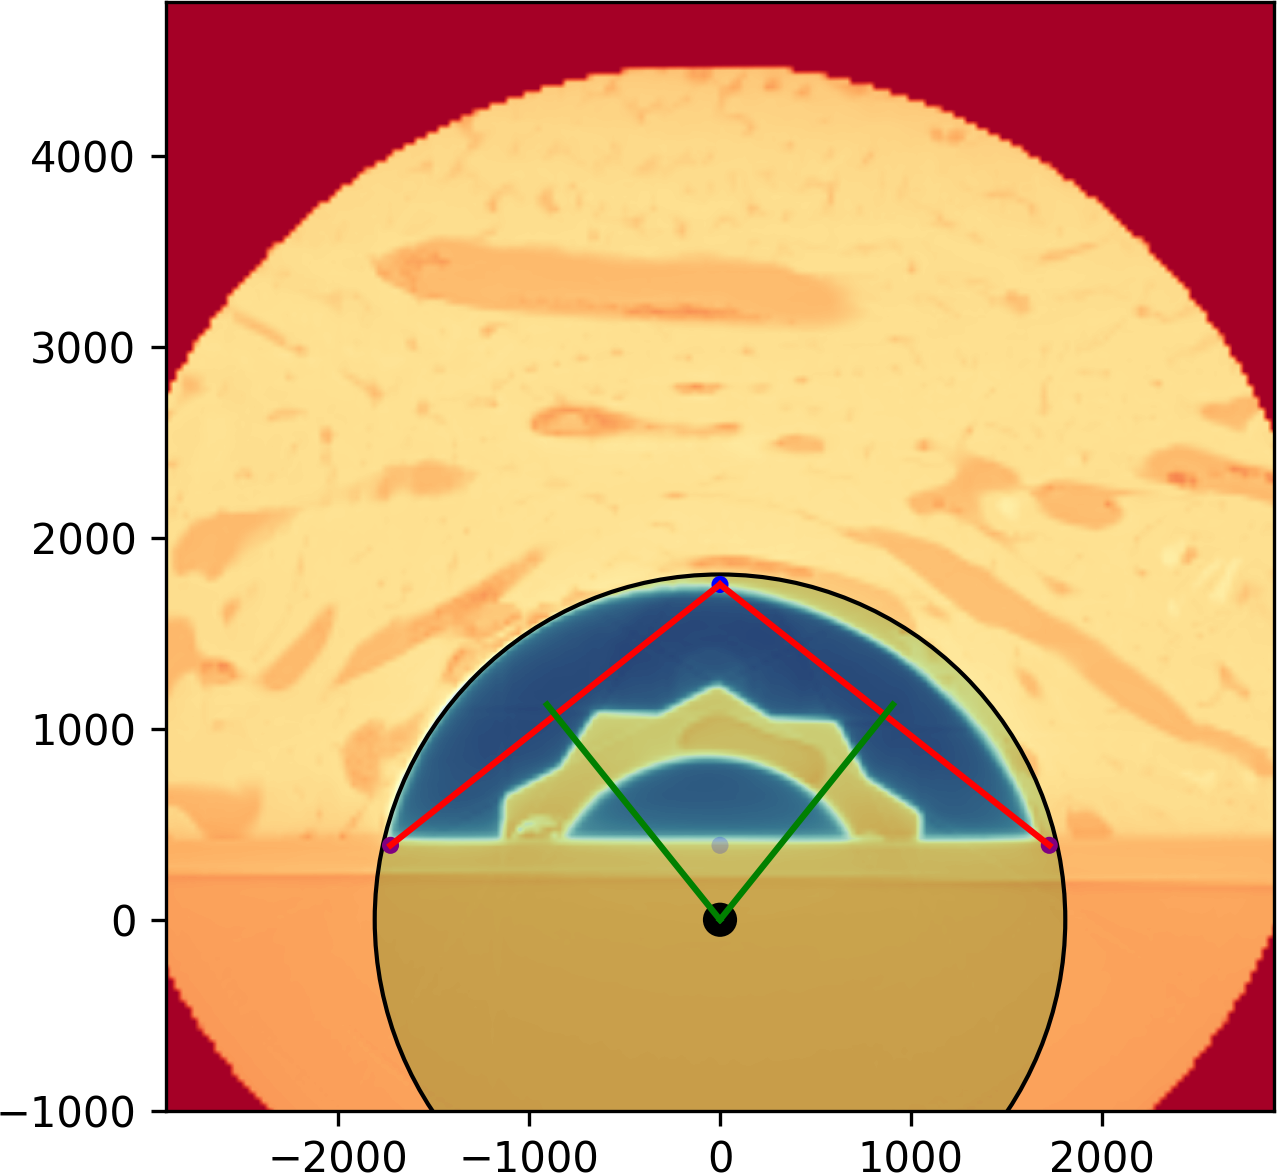
\includegraphics[width=.8\linewidth]{implant-FoR_prime-circle}\end{tabular} \\
%     (b) & \begin{tabular}{c}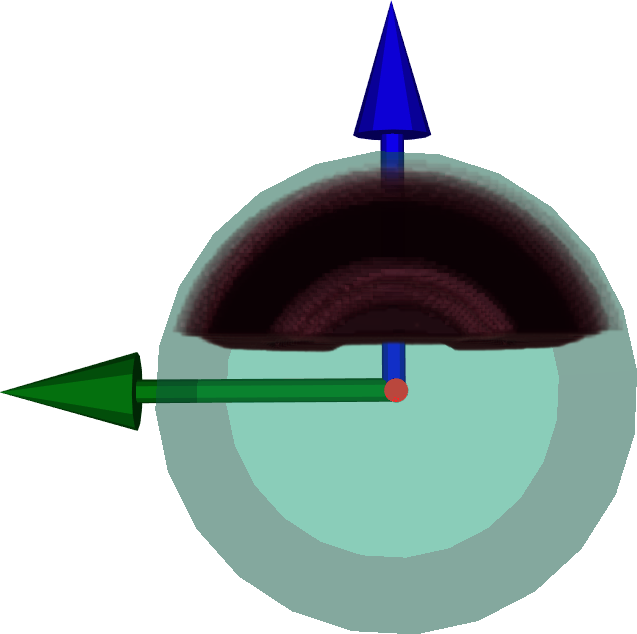
\includegraphics[width=0.4\linewidth]{implant-FoR_cylinder-y}%
%   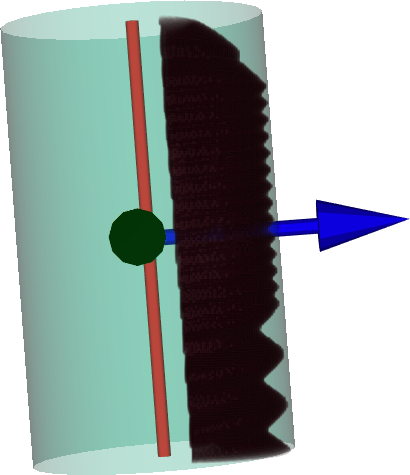
\includegraphics[width=0.5\linewidth]{implant-FoR_cylinder-z2}\end{tabular}
%   \end{tabular}
%   \caption{
%     (a) The implant is divided into 100 segments along its principal axis,
%     and for each segment, the circumscribed circle is computed.
%     (b) The best overall cylindrical fit for the implant is computed using
%     least squares. The implant contact is projected onto this cylinder,
%     and can now be shown in a flat plot.}
%   \label{fig:cylinder1}
% \end{figure}





%%% Local Variables:
%%% mode: latex
%%% TeX-master: "main"
%%% End:


\section{Conclusion and future work}
\label{sec:conclusion}

While SRµCT yields 3D reconstructions of extremely high quality compared to
lab-scale X-ray setups, several distortive effects remain that obstruct
accurate tissue classification in important regions, in particular near and at
interfaces of high-contrast transitions such as where biological tissue meets
metallic implants. However, these effects are well-behaved, in the sense that
they vary smoothly over space, making it possible to discover approximate
mathematical models of the effects and counter their resulting distortion.

We were able to build probabilistic models for the distortive effects of soft
tissue and bone voxel values as functions of distance to the implant and as
functions of an approximate diffusion field. This made it possible to see close
to the implant surface, and automatically segment into tissue types throughout
the sample and all the way up to the implant surface, with high accuracy both
at long and short distances.

In this pilot work, we have only looked at utilizing the combined field and
distance transform to the implant surface. We have not yet compared the results
to histology microscopy, which is the gold standard for tissue classification.
However, the results are promising: the segmentation is successful, and the
tissue-to-implant contact can be studied quantitatively and qualitatively. The
method is also general and can be applied to other types of samples with
similar distortion effects.

In upcoming work, we plan a larger quantitative study that compares with
histology microscopy results, obtained from the same biopsies. In addition, we
are extending the method with a Bayesian combination of multiple ``angles'':
different sources of distortion effects (e.g. multiple physical effects) can be
better captured by different fields, e.g. implant-glow may be best captured
by the distance transform to the sample surface, while the diffusion field
captures distortion near metallic implants. Thus, different fields separate
tissue material distributions in different regions and are expected to yield a
stronger analysis when combined. It is hoped that this will make it possible to
separate multiple highly overlapping frequency distributions.

\section{Data availability}

% TODO (James): ERDA eller?
Original data and synthetic data, with STL files and ground truth have been
made freely available.

\section{Acknowledgements}

This project has received funding from the European Union’s Horizon 2020
research and innovation programme under grant agreement No.~779322
(``MAXIBONE'').  JA was partially funded by VILLUM FONDEN (VILLUM Experiment
no.~23321, “Folding Carbon: A Calculus of Molecular Origami”).  CJ was partially
funded by the Innovation Fund Denmark (IFD) under File No.~8057-00012B, the IFD
Grand Solutions project ``Adaptive X-ray InSpection''.  JA, AT and CJ was funded
by the VILLUM Foundation through (VILLUM Experiment no.~41017, “OsteoMorph:
Understanding Bone Microphysics through Computational Morphology of SRuCT”).

\section{Conflict of Interest}
On behalf of all authors, the corresponding author states that there is no
conflict of interest.

%%% Local Variables:
%%% mode: latex
%%% TeX-master: "main"
%%% End:


\bibliographystyle{model2-names.bst}\biboptions{authoryear}
\bibliography{refs}
\end{document}
